% !TEX root = ../main.tex
\section{Tuning}
\label{sec:04_Tuning}

The Convolutional Neural Network, described and implemented in Chapter \ref{sec:03_Convolutional_Neural_Network}, provides the starting point for the numerical study presented in this Chapter. Although the initial model is already able to approximate the lift coefficient from the airfoil geometry and the flow parameters, we decided to understand which choice of architecture, optimization algorithm, regularization, activation function and learning rate allow the surrogate model to obtain more accurate and more reliable predictions. For this reason, we performed a sequence of controlled tuning experiments. In each experiment one group of quantities was varied, while the other settings were kept fixed. The results were then analysed not only through the final validation error, but also through the evolution of the training objective, the physical validation error, the gradient norms, the actual parameter updates and the activation distributions.\\

The order of the study follows the development of the model:
\begin{itemize}
    \item[-] first, we investigated the topology of the network, because the feature representation and the capacity of the regression head influence every subsequent experiment;
    \item[-] then, we considered dropout, the optimizer, the weight of the SIMM physical term, and L1 and L2 regularization;
    \item[-] next, we compared the available activation functions;
    \item[-] as last thing, we studied the magnitude and the schedule of the learning rate.
\end{itemize}
The last part of the Chapter (Section \ref{sec:04_final_training}) describes the recorded ordinary training sequence and its final production configuration, and collects the conclusions that can be drawn from the complete tuning.

\subsection{Cross-validation and diagnostic methodology}
\label{sec:04_cross_validation}

All the tuning experiments use the training dataset stored in \texttt{dataset/cnn\_dataset\_train.npz}\footnote{Both the training and test datasets are generated according to the procedure detailed in Section \ref{sec:02_Navier-Stokes_Simulation}.}, which contains 1713 samples. Each sample consists of a $150\times150$ Signed Distance Function\footnote{See Section \ref{sec:03_SDF} for details about the implementation.}, the scalar pair $(\mathrm{Re},\alpha)$ and the corresponding lift coefficient $C_L$. The separate file \texttt{dataset/cnn\_dataset\_test.npz}, containing 429 samples, is not used to compare candidates. In the intended procedure, it is loaded only after a candidate has been selected and the selected model has been refitted on the complete training dataset. This separation is important because using test data during the search would turn the final error into a selection quantity rather than an independent estimate.\\

The comparisons are performed with the project implementation of \texttt{RandomKFold}. The samples are shuffled with a fixed seed and divided into five folds. An important detail is that the data is split on a per-sample basis, meaning individual simulation results are distributed randomly rather than grouping all data from a single airfoil into one fold. This means that for any given fold, data from the same airfoil (e.g., NACA 0012) can appear in both the training and validation sets. In this way, the tuning experiments measure the model's ability to interpolate within the dataset, rather than its capacity for generalization to entirely new airfoil families. This per-sample choice is intentional: the project track defines the surrogate task as prediction over $(\mathrm{Re},\alpha)$ for the airfoils included in the dataset, not zero-shot transfer to unseen geometries. In every fold, approximately eighty percent of the samples are used for training and the remaining twenty percent for validation. In the recorded runs, the validation sets contain 342 (or 343 samples) and the training sets contain 1370 (or 1371 samples). The fold plan is generated once and reused for every candidate within a tuning experiment, guaranteeing that every candidate model is benchmarked on the exact same data for a direct comparison.\\

The experimental procedure enforces the following key principles, in order to ensure reproducible comparisons.\\

First of all, the normalization statistics (such as mean and standard deviation) are calculated exclusively from the training data. These same statistics are then used to scale the validation data. We also added a minor preprocessing step to convert the angle of attack from degrees to radians, which is necessary for the physics-informed loss function. Next, every trial is completely independent. For each candidate model and each fold, a new instance of the network and optimizer is created from scratch, in order to not carry over any learned parameters, optimizer moments or any other state from previous runs. Finally, the distributed training framework is designed to be consistent. The global batch size is fixed for all experiments, and increasing the number of MPI processes simply divides this global batch into smaller sub-batches for each worker. This ensures that the results and metrics are independent of the number of parallel ranks used.\\

To execute the extensive hyperparameter sweeps in an automated, scalable and reproducible manner, we engineered a modular, object-oriented \cpp framework. The core of this framework is a "recipe-and-blueprint" design pattern, which decouples the abstract specification of a model from its physical runtime instantiation.\\

This process beings with \texttt{LayerRecipe} instances, which define each layer not as an object, but as a set of instructions. Each recipe encapsulates two core functionals:
\begin{itemize}
    \item[-] a shape inference mapping to dynamically compute output tensor dimensions;
    \item[-] a deferred builder to allocate and initialize the layer's parameters from a deterministic seed.
\end{itemize}
A \texttt{ModelBlueprint} then assembles these recipes into a complete network structure, logically separated into a convolutional feature extraction trunk and a fully-connected regression head.\\

To systematically generate the wide range of candidates for our sweeps, a parametric factory function, \\\texttt{make\_blueprint}, constructs these blueprints on the fly. It accepts a full set of architectural parameters (such as kernel sizes, dense head widths and dropout rates) and chains together the appropriate recipes to produce a complete and custom \texttt{ModelBlueprint}.\\

A complete experimental candidate is then defined by a \texttt{TrialConfig} structure. This object bundles the \texttt{ModelBlueprint} with an \texttt{OptimizerRecipe} (e.g., Adam, SGD), a learning rate scheduler and all other loss and training settings. A \texttt{SearchSpace} utility then generates a full list of these \texttt{TrialConfig} objects, defining the entire grid for a given tuning experiment.\\

Orchestration is handled by the \texttt{CrossValidator} object. For each candidate \texttt{TrialConfig}, it executes the complete K-fold scheme. Crucially, for every fold, it uses the blueprint and recipes to instantiate a completely new, isolated model and optimizer. This deferred, just-in-time instantiation guarantees strict isolation and ensures zero state carryover between folds or candidates. Finally, the training loop itself is managed by the \texttt{Trainer}, which enforces our balanced batching and "20/20" early stopping rules, while a concurrent \texttt{TrainingDiagnostics} module captures the detailed stability metrics analyzed throughout this chapter.\\

With this experimental framework and software infrastructure established, we evaluate each candidate using a primary selection metric, supplemented by a series of diagnostic quantities to analyze model behavior.\\

The primary selection quantity is the physical-unit mean squared error on the validation samples. If $\hat{C}_{L,i}$ is the predicted coefficient and $C_{L,i}$ is the CFD value, the physical MSE of fold $k$ is computed as:
\begin{equation}
    \mathrm{MSE}_{\mathrm{val}}^{(k)} =
    \frac{1}{n_k}\sum_{i\in\mathcal{V}_k}
    \left(\hat{C}_{L,i}-C_{L,i}\right)^2
    \label{eq:04_validation_mse}
\end{equation}
where $\mathcal{V}_k$ is the validation subset and $n_k$ is its number of samples.\\

The final score for a candidate is the sample-weighted 
average of this MSE across all five folds, as returned by \texttt{CrossValidator}. This distinction matters because the training objective contains a data term and, in some experiments, a physics term expressed in fold-specific standardized target units, while Equation \eqref{eq:04_validation_mse} is expressed in the squared physical lift-coefficient units. To assess the sensitivity of a model to the specific data split, the standard deviation of the MSE across folds is also reported alongside the mean.\\

Beyond the primary selection metric, we monitor several diagnostic quantities to ensure numerical stability and understand the training dynamics. The training objective is monitored through \texttt{train\_objective}, while the physical training and validation errors are read from \texttt{epoch\_metrics.csv}. The cross-validation history is normally stored every ten epochs, although diagnostics contain a validation value at every epoch.\\

The following diagnostic quantities are used throughout the Chapter:
\begin{itemize}
    \item[-] the gradient norm is read from rows with \texttt{parameter\_scope=all} and it is measured after the MPI weighted gradient aggregation and before clipping and the optimizer update. This metric indicates whether gradients are naturally vanishing or exploding;
    \item[-] the parameter update ratio is the actual movement of the parameters relative to their norm, computed as:
    \begin{equation}
    r_{\theta} =
    \frac{\lVert\theta_{\mathrm{after}}-\theta_{\mathrm{before}}\rVert_2}
    {\max\left(\lVert\theta_{\mathrm{before}}\rVert_2,10^{-12}\right)},
    \label{eq:04_update_ratio}
\end{equation}
    where $\theta_{\mathrm{before}}$ and $\theta_{\mathrm{after}}$ are the parameter vectors before and after the optimizer update, respectively.\\
    A healthy value typically hovers around $10^{-3}$. Excessively high values point to numerical instability or an overly aggressive learning rate, whereas excessively low values indicate training stagnation. The $10^{-12}$ term serves as a safety epsilon to prevent division by zero.
    \item[-] the pre-activation and post-activation statistics are computed for every layer, including the mean, variance, minimum, maximum, and fixed-bin histograms of the activation tensors;
    \item[-] the activation statistics are distinguished between the pre-activation tensor entering a non-linearity and the post-activation tensor returned by it. Their mean, variance, minimum, maximum and fixed-bin histograms are used to identify signal attenuation, saturation, or growth of the activation scale.
\end{itemize}
In all cases, we checked the raw CSV files for non-finite values and for late-epoch increases before describing a run as numerically stable.

\subsection{Topology tuning}
\label{sec:04_topology_tuning}

The first tuning activity concerned the topology of the network, as it dictates the model's fundamental capacity to learn from the data. The architecture has two key components:
\begin{itemize}
    \item[-] a convolutional feature extractor responsible for extracting meaningful geometric features from the $150\times150$ SDF input;
    \item[-] a dense head that fuses these geometric features with the scalar flow parameters (Reynolds number and angle of attack) to predict the final lift coefficient.
\end{itemize}
The main focus is to find the right balance. A model with insufficient capacity (too few layers or neurons) may fail to capture the non-linear relationship between an airfoil's shape and its aerodynamic performance. Conversely, an overly complex model risks poor generalization, fitting noise in the training data rather than the underlying physical principles, while also increasing computational cost.\\

This type of structural comparison is consistent with the surrogate model motivation introduced in Chapter~\ref{sec:03_Convolutional_Neural_Network}. The reference to the role of activation and gradient propagation in deep networks discussed by \cite{glorot2010understanding} is kept here only as motivation for studying signal propagation in principle, since that work considers saturating nonlinearities and initialization and does not predict a kernel size or a head width for this SDF trunk.\\

This experiment systematically explores different architectural choices, such as the convolutional kernel size, the width and depth of the dense head, to identify a topology that optimally balances representational power with generalization performance. All other hyperparameters, such as the optimizer and loss function, were held constant to isolate the impact of the architecture itself.\\

For the convolutional trunk, we evaluated different kernel sizes, which directly govern the spatial resolution of the resulting feature maps and, consequently, the input dimensionality to the dense head. For a two-dimensional convolution with input size $H_{\mathrm{in}}\times W_{\mathrm{in}}$, kernel size $K$, stride $S$, and zero padding $P$, the output dimensions are
\begin{equation}
    H_{\mathrm{out}} = \frac{H_{\mathrm{in}}-K+2P}{S}+1,
    \qquad
    W_{\mathrm{out}} = \frac{W_{\mathrm{in}}-K+2P}{S}+1.
    \label{eq:04_topology_convolution}
\end{equation}
The topology experiment used $P=0$ and set the stride equal to the kernel size, with eight output channels in every candidate. The two main alternatives for the trunk were a $5\times5$ kernel (producing a $30\times30$ feature map, leading to $7202$ inputs for the dense head) and a $3\times3$ kernel (producing a $50\times50$ feature map, leading to $20002$ inputs for the dense head).\\

For the dense head, we explored variations in both width (the number of neurons in each layer) and depth (the number of hidden layers). A head with widths $(w_1,\ldots,w_m)$ then applies successive transformations $\mathbf{h}_{j+1}=\sigma(W_j\mathbf{h}_j+\mathbf{b}_j)$ with LeakyReLU nonlinearity $\sigma$ and ends with a linear scalar output. Increasing the widths mainly affects the capacity of the first dense transformation, while adding hidden layers changes the depth of the nonlinear mapping. 
The parameter count makes this distinction concrete. With the $5\times5$:
\begin{itemize}
    \item[-] the baseline head $(128,64)$ holds 930305 parameters;
    \item[-] the intermediate head $(512,256)$ holds 3819521 parameters;
    \item[-] the selected head $(1024,512,256,128)$ holds 8065025 parameters;
    \item[-] the widest depth two head $(2048,1024)$ holds 16850945 parameters.
\end{itemize}
Each dense layer contributes $(D_{\mathrm{in}}+1)D_{\mathrm{out}}$ weights and biases and the convolution contributes $(K^2+1)\times 8$ parameters.\\

To systemically evaluate these architectural trade-offs, we designed a comprehensive grid search. The search contained 18 candidates and therefore 90 fold evaluations. Each fold was trained following the same recipe:
\begin{itemize}
    \item[-] 100 epochs with global batch size 64;
    \item[-] Adam optimizer with learning rate $10^{-5}$;
    \item[-] a SIMM physics weight of $0.25$;
    \item[-] LeakyReLU activation with negative slope $0.05$.
\end{itemize}
The baseline was \texttt{conv5x5-dense-128-64}. The entire experiment was conducted following the rigorous cross-validation framework, evaluation metrics and rules detailed in Section \ref{sec:04_cross_validation}.\\

The official results and logs for this specific search are committed in the CINECA Leonardo log \\\texttt{run\_leonardo\_51807287.log} and its corresponding summary files. It should be noted that detailed per-epoch diagnostic logging (e.g. gradient norms, activation statistics) was disabled for this particular grid search. The only convergence histories are the public ten epoch checkpoints printed to the log.\\

The results of the 90-fold evaluation, summarized in Table \ref{tab:04_topology_results}, reveal the trends regarding the impact of network architecture on prediction accuracy. The ranked performance of all candidates is shown in Figure \ref{fig:04_topology_ranking}.\\

\begin{table}[h!]
    \centering
    \begin{tabular}{lcc}
        \hline
        Candidate & Mean validation MSE & Fold standard deviation \\
        \hline
        \texttt{conv5x5-dense-1024-512-256-128} & 0.004560 & 0.000946 \\
        \texttt{conv5x5-dense-1024-512-256-128-64} & 0.004626 & 0.000918 \\
        \texttt{conv5x5-dense-1024-512} & 0.004851 & 0.000911 \\
        \texttt{conv5x5-dense-512-256-128-64} & 0.004872 & 0.001125 \\
        \texttt{conv5x5-dense-512-256} & 0.005052 & 0.001067 \\
        \texttt{conv5x5-dense-1536-768} & 0.005307 & 0.001177 \\
        \texttt{conv5x5-dense-2048-1024} & 0.005673 & 0.001466 \\
        \texttt{conv5x5-dense-128-64} (baseline) & 0.006010 & 0.000823 \\
        \texttt{conv3x3-dense-128-64} & 0.006330 & 0.001099 \\
        \texttt{conv5x5-dense-64-32} & 0.006425 & 0.001292 \\
        \texttt{conv3x3-dense-512-256} & 0.006459 & 0.001318 \\
        \hline
    \end{tabular}
    \caption{Representative topology candidates in ranked order. The ranking was performed over the complete 18 candidate grid by sample-weighted mean physical validation MSE. The omitted intermediate candidates fall between the rows shown and do not change the conclusions.}
    \label{tab:04_topology_results}
\end{table}

The lowest observed validation MSE was obtained by \texttt{conv5x5-dense-1024-512-256-128}, with $0.004560\pm0.000946$. This represents a substantial improvement over the baseline \texttt{conv5x5-dense-128-64}, which achieved $0.006010\pm0.000823$, outperforming it consistently across all five cross-validation folds. The mean paired difference between the winner and the baseline is $-0.001450$, indicating an advantage of the selected topology. After being refit on the entire training dataset, this winning topology achieved an MSE of $0.002805$ on the untouched test dataset.\\

\begin{figure}[h!]
    \centering
    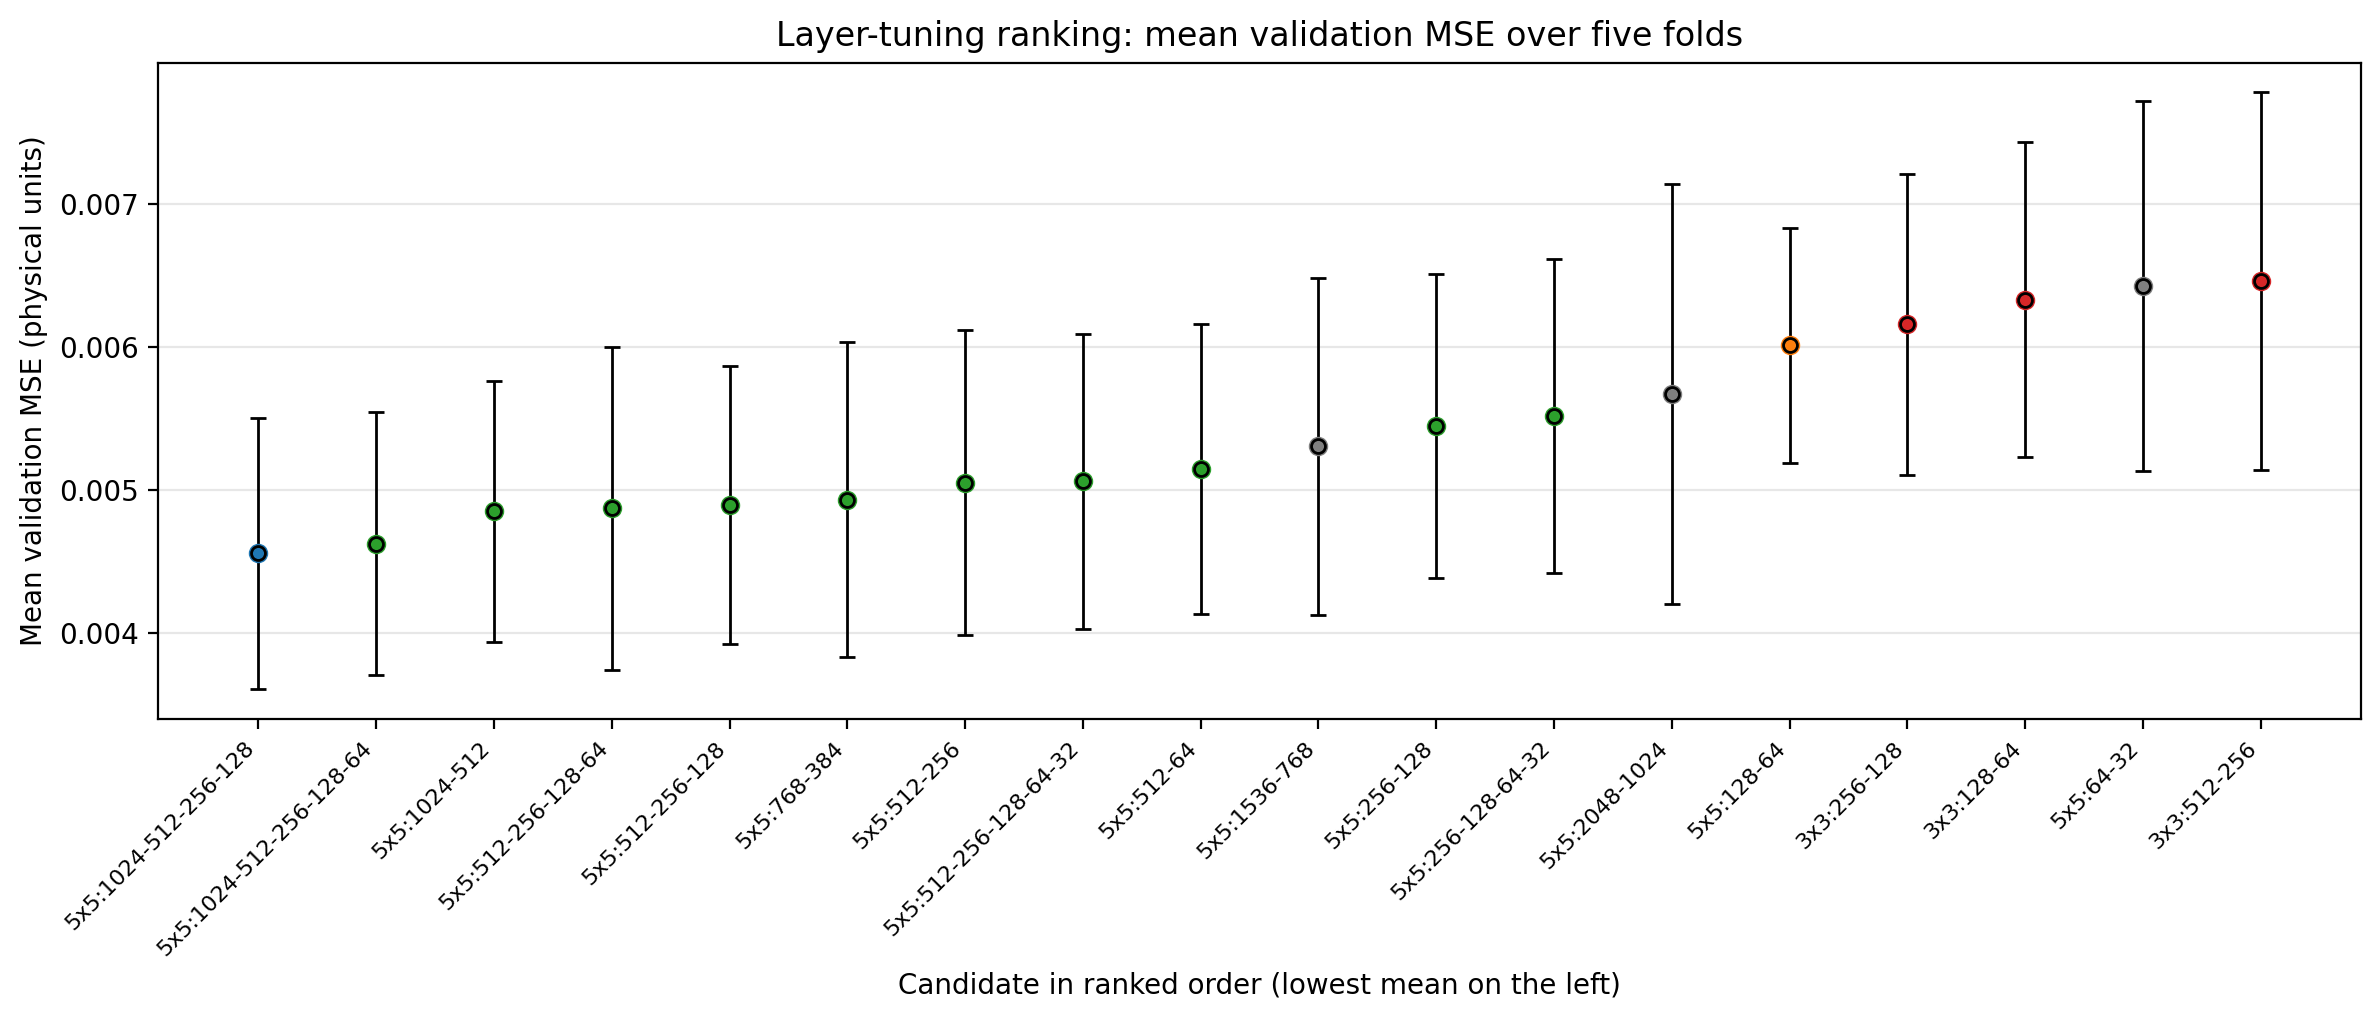
\includegraphics[width=0.95\linewidth]{Images/Chapter04/topology/topology_ranking.png}
    \caption{Layer tuning ranking by sample-weighted mean physical validation MSE over five folds. Error bars show the fold standard deviation. The leftmost candidate is the selected \texttt{conv5x5-dense-1024-512-256-128}. The plot summarizes \texttt{summary.csv} and does not imply a fitted scaling law.}
    \label{fig:04_topology_ranking}
\end{figure}

The analysis shows that both network width and depth were crucial for achieving this performance, but with diminishing returns.\\

Deeper networks consistently proved more effectivee at learning the complex relationship between airfoil geometry and lift coefficient. We can see that at entry width $(512,256)$, increasing the head from two to four hidden layers reduced the mean error from $0.005052$ to $0.004872$, while at entry width $(1024,512)$ the corresponding increase in depth reduced it from $0.004851$ to $0.004560$. Increasing width also helped at fixed depth, but the gains became smaller and then reversed. At a fixed depth of two layers, the MSE decreased steadily as the head widened from $(64,32)$ (with an MSE of $0.006425$) to $(1024,512)$ (with an MSE of $0.004851$). However, this trend then reversed. Increasing the width further to $(1536,768)$ caused the error to rise again to $0.005307$, and further to $(2048,1024)$ with an MSE of $0.005673$. This indicates that the model was becoming too large and was beginning to lose its generalization capability.\\

For this reason, the best performance is not achieved by maximizing either width or depth in isolation, but by finding an effective interaction between the two.\\

The kernel comparison gives a second clear result. Across all paired comparison, the $5\times5$ convolution consistently outperformed the $3\times3$ convolution. This trend is clearly visible in the paired comparisons shown in Figure \ref{fig:04_topology_kernel_paired}. For instance, when paired with the $(512,256)$ dense head, the $5\times5$ kernel achieved a mean MSE that was lower by approximately $0.001407$ compared to the $3\times3$ kernel. This outcome is likely due to the larger receptive field of the $5\times5$ kernel. With a larger window, the model can capture broader spatial patterns and more complex geometric details from the SDF input in a single step, useful for the prediction of the lift coefficient.\\

The convergence history, shown in Figure \ref{fig:04_topology_history}, further supports this conclusion. Models using the $5\times5$ kernel consistently achieved lower validation MSEs throughout the training process, indicating that they were able to learn more effectively from the data.\\

\begin{figure}[H]
    \centering
    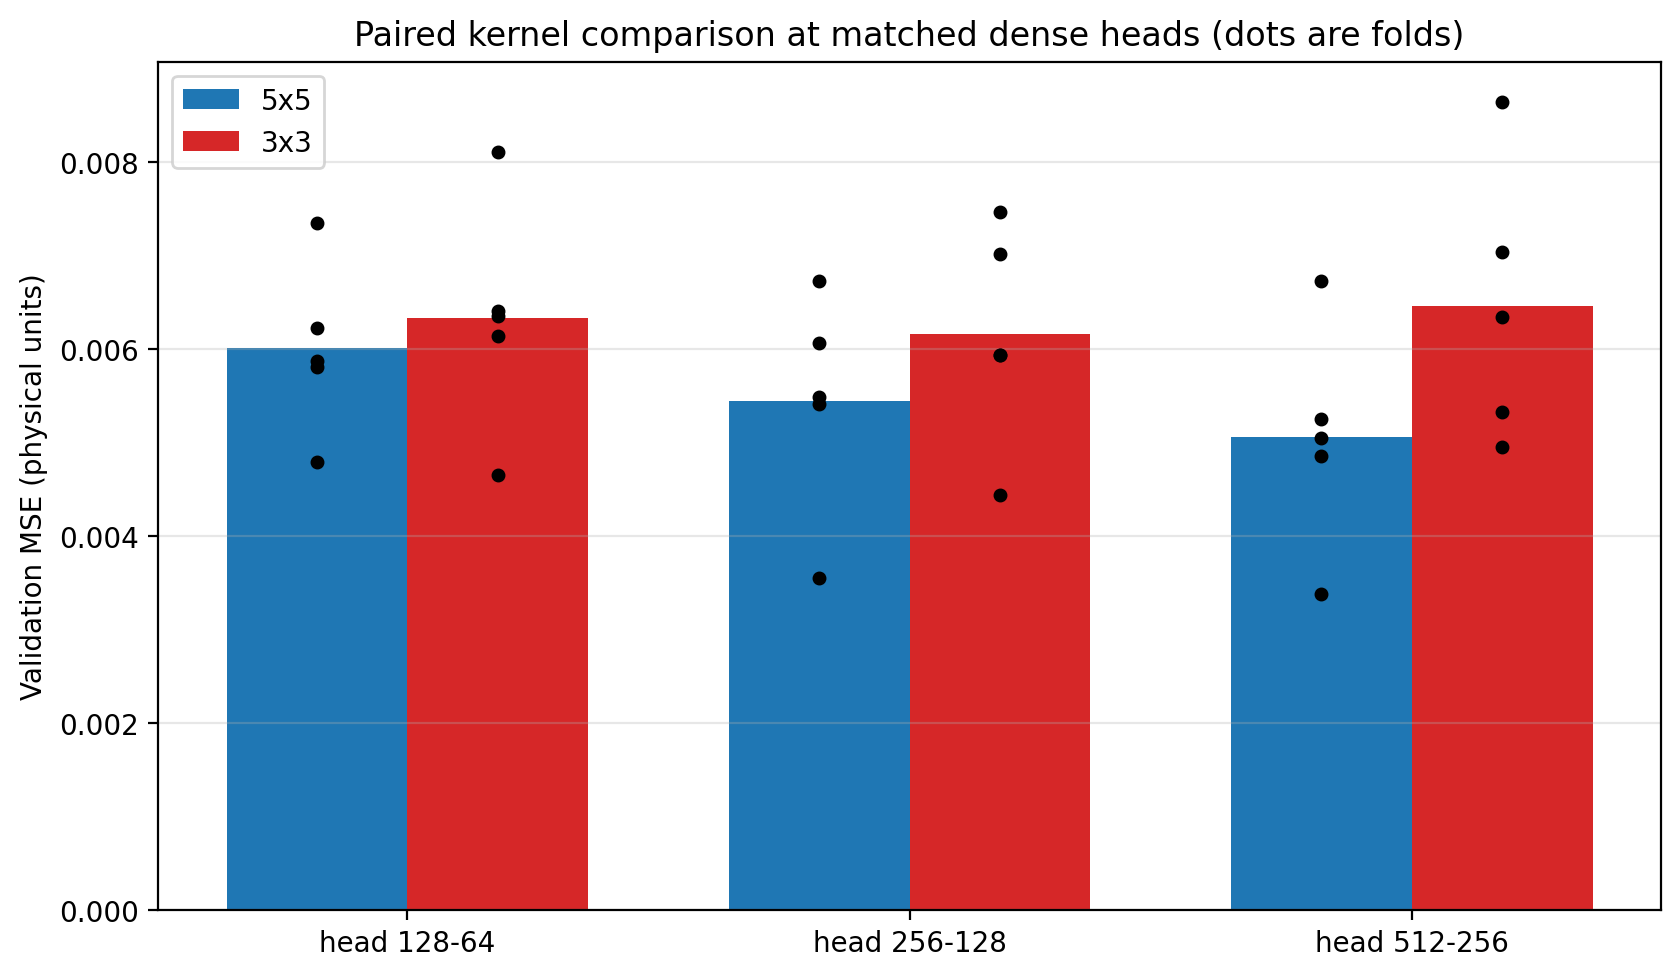
\includegraphics[width=0.65\linewidth]{Images/Chapter04/topology/topology_kernel_paired.png}
    \caption{Paired kernel comparison at three matched dense heads. Bars show the sample-weighted mean physical validation MSE and dots show the five per fold values from \texttt{aggregated.csv}. All three pairs favour $5\times5$ with stride five over $3\times3$ with stride three at zero padding.}
    \label{fig:04_topology_kernel_paired}
\end{figure}

\begin{figure}[H]
    \centering
    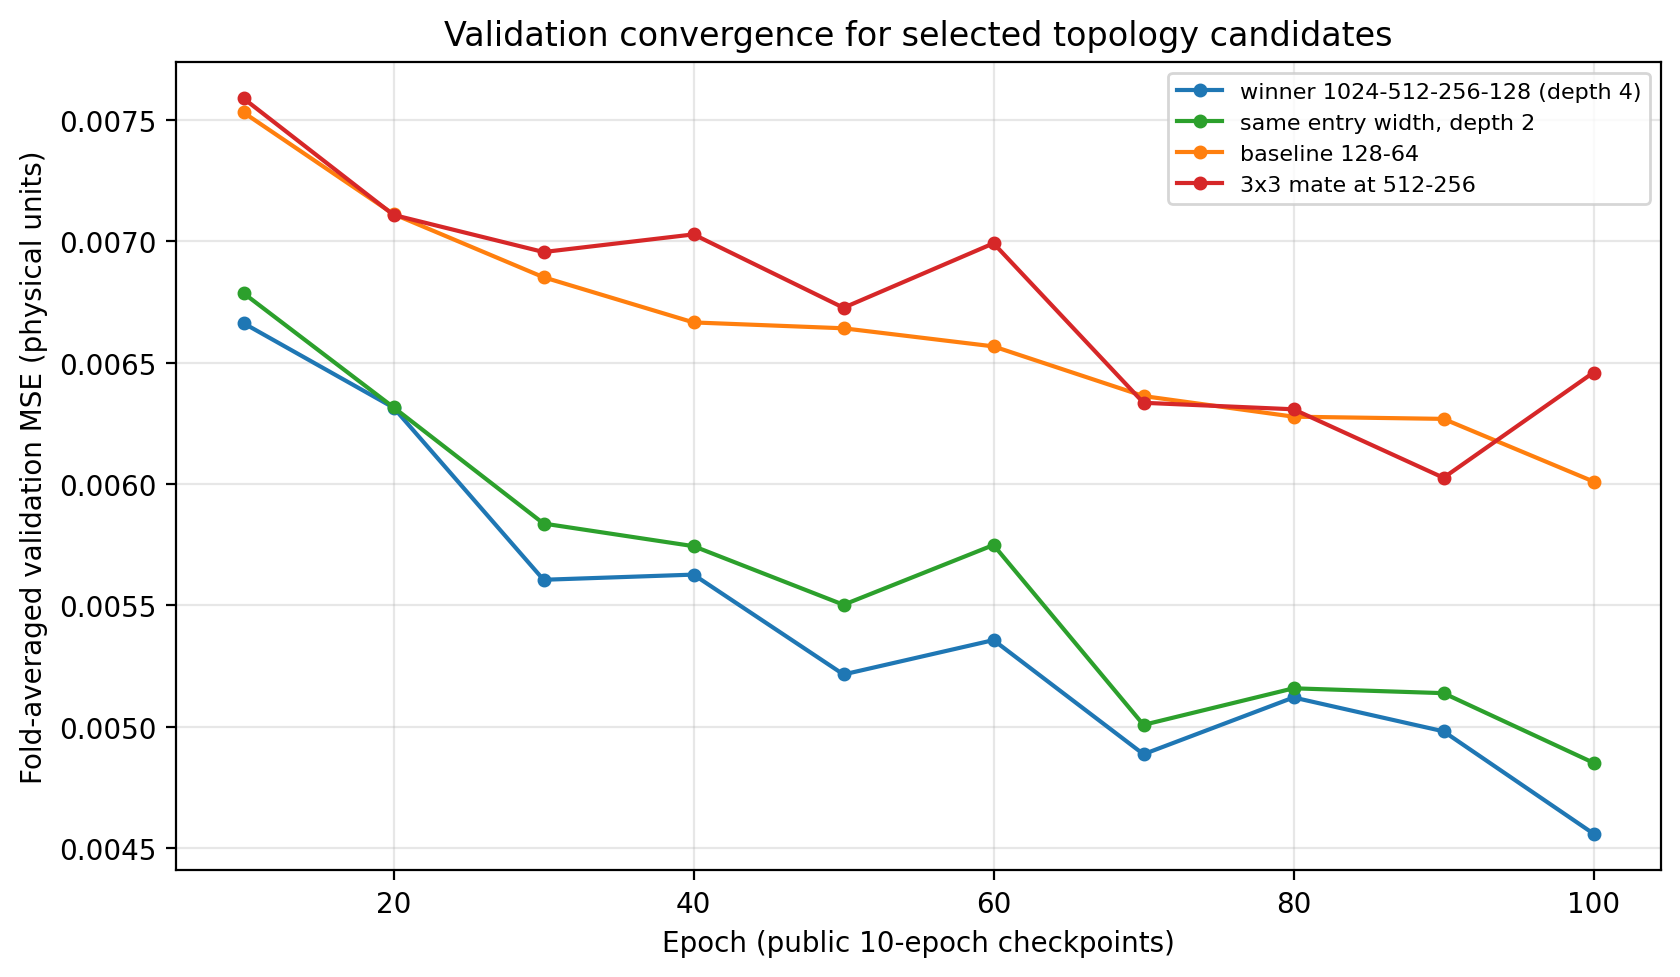
\includegraphics[width=0.65\linewidth]{Images/Chapter04/topology/topology_history.png}
    \caption{Fold averaged physical validation MSE at public checkpoints every ten epochs. Curves are shown for the winner \texttt{conv5x5-dense-1024-512-256-128}, the depth two candidate \texttt{conv5x5-dense-1024-512}, the baseline \texttt{conv5x5-dense-128-64}, and the $3\times3$ mate \texttt{conv3x3-dense-512-256}. The training objective is omitted because it uses different standardized units.}
    \label{fig:04_topology_history}
\end{figure}

However, it is important to acknowledge several limitations inherent to this specific experimental setup:
\begin{itemize}
    \item[-] as already said in Section \ref{sec:04_cross_validation}, this grid search was executed without recording detailed per-epoch diagnostics. While all runs completed successfully without signs of divergence, this prevents a deeper analysis of phenomena like vanishing or exploding gradients for these specific candidates;
    \item[-] each candidate was trained only once per fold with a fixed random seed. Consequently, architecture difference cannot be separated from training seed noise;
    \item[-] as established in our methodology (Section \ref{sec:04_cross_validation}), the training and validation sets are split at the sample level, meaning that data from the same airfoil can appear in both sets. This setup measures interpolation within the dataset rather than generalization to unseen airfoil families;
    \item[-] the grid search was limited to a specific range of kernel sizes, head widths, and depths. While the selected candidate performed best within this grid, it is possible that other configurations outside this range could yield even better results.
\end{itemize}
\vspace{2ex}

The cross-validation winner is \texttt{conv5x5-dense-1024-512-256-128}, with physical validation MSE $0.004560\pm0.000946$ and untouched test MSE $0.002805$ after refitting on the complete training set. 

\subsection{Dropout tuning}
\label{sec:04_dropout_tuning}

Dropout is a regularization technique designed to prevent overfitting in large networks by randomly deactivating neurons during training, which discourages complex co-adaptations between them, as shown by \cite{srivastava2014dropout}. Typically, it is most effective when there is a clear gap between training and validation performance. The preceding regularization experiment, however, showed only a small training to validation gap relative to the fold variability. The dropout experiment therefore tests a specific question: can stochastic masking improve validation accuracy when the available evidence does not indicate a large deterministic overfitting gap?\\

During training, a random subset of activations in a layer is set to zero. The remaining are scaled up by the reciprocal of the survival probability to maintain the expected magnitude of the layer's output. This process, which effectively trains a large ensemble of thinned subnetworks, can be expressed mathematically as:
\begin{equation}
    \widetilde{z}_j = \frac{m_j}{1-p}z_j,
    \qquad m_j\sim\mathrm{Bernoulli}(1-p)
    \label{eq:04_dropout}
\end{equation}
where $p$ is the probability of dropping an element and $1-p$ is the survival probability. The same scaled mask is used during backpropagation, so that:
\begin{equation}
    \frac{\partial L}{\partial z_j} =
    \frac{m_j}{1-p}\frac{\partial L}{\partial\widetilde{z}_j}
    \label{eq:04_dropout_backward}
\end{equation}
At inference, the mask is disabled and the layer is the identity, so no additional rescaling is needed.\\     

In the implementation, a \texttt{DropoutLayer} is inserted after every hidden \texttt{LeakyReLULayer} within the dense regression head. It is not applied to the final scalar output. The tested grid was $p\in\{0,0.1,0.2,0.3,0.5\}$, including the baseline case of no dropout.\\

To isolate the effect of dropout, all other hyperparameters were held constant, retaining the winning topology from Section \ref{sec:04_topology_tuning}. The experiment strictly followed the established cross-validation protocol detailed in Section \ref{sec:04_cross_validation}, using the Adam optimizer (learning rate of $10^{-5}$), a SIMM physics weight of $0.25$, batch size 64 and a 100-epoch budget across identical data folds.\\

For rigorous reproducibility, the dropout masks are generated deterministically from a combination of the fold seed, epoch, sample row, and feature index. This design ensures that the stochastic mask remains identical regardless of the number of parallel MPI ranks employed. Crucially, the baseline candidate ($p = 0.0$) retains the dropout layer as an identity mapping rather than omitting it. This guarantees that all candidates share identical parameter initializations and random number sequences. Consequently, the resulting baseline performance is strictly paired within this sweep and should not be compared directly against standalone runs configured without the identity layer.\\

Candidate selection used the sample-weighted physical-unit validation MSE returned by \texttt{CrossValidator}. The official aggregate file is \texttt{cv\_summary.csv}; the paired differences, final training MSE, and training to validation gaps are read from \texttt{sweep\_dropout.csv}. The two files differ slightly in their arithmetic means because the official score weights the 342 and 343 sample validation folds, while the sweep CSV is also used to preserve the fold-by-fold paired inputs. Table \ref{tab:04_dropout_results} reports the complete grid. The last three columns are descriptive quantities and do not replace the physical validation MSE as the selection metric.\\

\begin{table}[h!]
    \centering
    \begin{tabular}{rccccc}
        \hline
        $p$ & Mean val. MSE & Fold std. & Paired $\Delta$ & Mean train MSE & Val. $-$ train \\
        \hline
        0.0 & 0.005834 & 0.001007 & 0.000000 & 0.005421 & +0.000413 \\
        0.1 & 0.006686 & 0.001060 & +0.000852 & 0.006390 & +0.000296 \\
        0.2 & 0.007630 & 0.000861 & +0.001796 & 0.007236 & +0.000395 \\
        0.3 & 0.008467 & 0.001141 & +0.002632 & 0.008098 & +0.000369 \\
        0.5 & 0.011764 & 0.002603 & +0.005930 & 0.011354 & +0.000411 \\
        \hline
    \end{tabular}
    \caption{Complete recorded dropout sweep. Mean validation MSE and fold standard deviation are the sample-weighted values from \texttt{cv\_summary.csv}. Paired differences, training MSE, and validation minus training gaps are calculated from \texttt{sweep\_dropout.csv}; a positive paired difference means that the rate is worse than the $p=0$ reference.}
    \label{tab:04_dropout_results}
\end{table}
\vspace{2ex}

The lowest validation error was achieved with dropout disabled ($p=0$), yielding a mean MSE of $0.005833893\pm0.001006787$. As shown in Figure \ref{fig:04_dropout_ranking}, performance systematically degraded as the dropout rate increased. Even a small rate of $p=0.1$ increased the error by nearly $15\%$, while the strongest rate of $p=0.5$ more than doubled the validation MSE.\\

\begin{figure}[H]
    \centering
    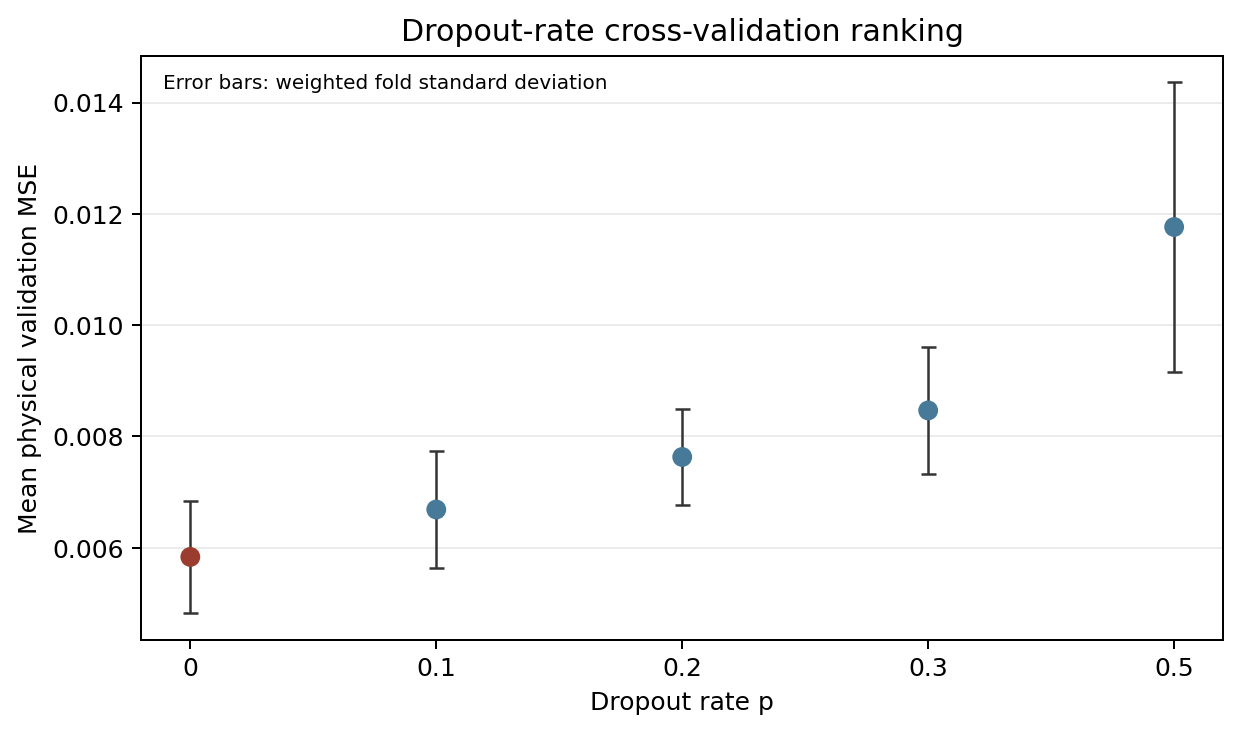
\includegraphics[width=0.78\linewidth]{Images/Chapter04/dropout/dropout_ranking.png}
    \caption{Dropout-rate ranking from the official \texttt{cv\_summary.csv}. Points are sample-weighted mean physical validation MSE and error bars are the weighted standard deviations over the five folds. The $p=0$ reference is highlighted in red.}
    \label{fig:04_dropout_ranking}
\end{figure}

This conclusion was remarkably consistent across all data splits. As visualized in the paired difference plot (Figure \ref{fig:04_dropout_paired}), no non-zero dropout rate improved performance in any of the five cross-validation folds.\\

\begin{figure}[h!]
    \centering
    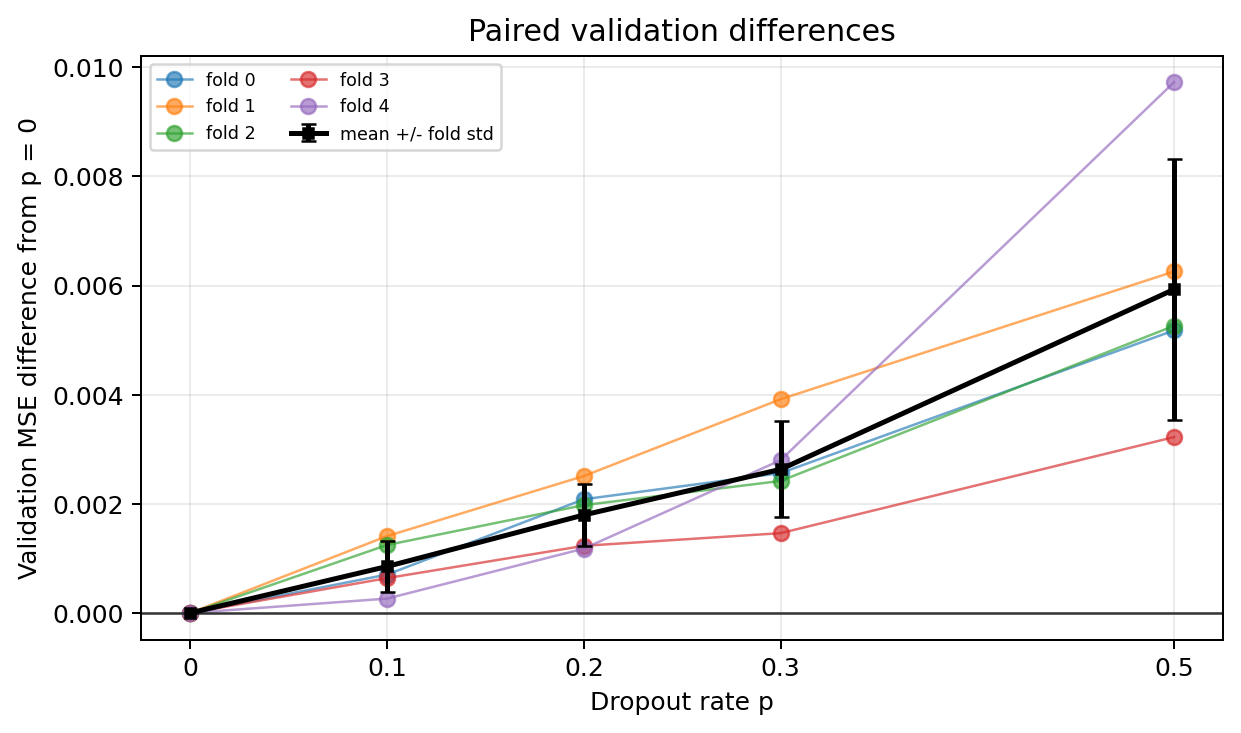
\includegraphics[width=0.78\linewidth]{Images/Chapter04/dropout/dropout_paired_differences.png}
    \caption{Paired physical validation MSE differences relative to the $p=0$ reference, computed from \texttt{sweep\_dropout.csv}. Coloured curves show the five zero-based folds, while black markers and error bars show the mean paired difference and its sample standard deviation. Positive values indicate deterioration relative to the reference.}
    \label{fig:04_dropout_paired}
\end{figure}

This outcome directly answers the experimental question posed in our motivation. For the baseline model ($p=0.0$), the gap between training and validation error was already very small ($+0.000413$), indicating no significant overfitting problem. While a small dropout rate ($p=0.1$) did slightly reduce this gap (to $+0.000296$), this minor improvement came at the cost of a much larger increase in the overall validation error.\\

This pattern strongly suggests that, for this well-specified architecture and dataset, dropout did not act as a useful regularizer. Instead, it functioned primarily as optimization noise, hindering the model's ability to converge to an accurate solution within the fixed 100-epoch training budget. Therefore, the evidence from this experiment supports disabling dropout entirely for the production model.\\

A closer look at the training dynamics, presented in Figure \ref{fig:04_dropout_history}, reinforces this conclusion. The training history reveals that all candidates converge stably, but to different levels: the final mean is approximately 0.0123 for $p=0$ and 0.1142 for $p=0.5$. These objective values are in standardized SIMM units and are not numerical alternatives to the physical validation MSE.\\

\begin{figure}[H]
    \centering
    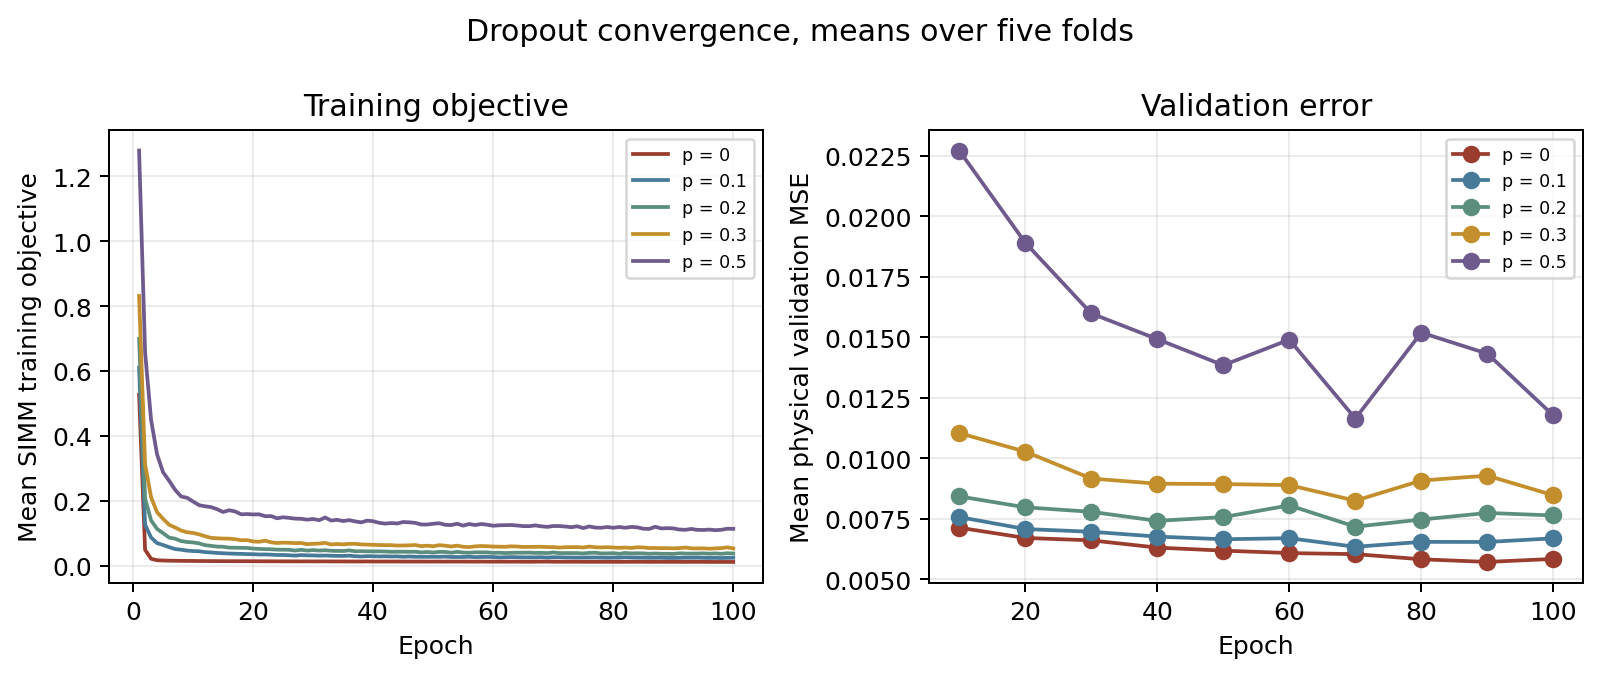
\includegraphics[width=0.95\linewidth]{Images/Chapter04/dropout/dropout_history.png}
    \caption{Means over the five recorded folds for the training SIMM objective and the physical validation MSE. The training objective is recorded at every epoch, whereas the validation values in the committed diagnostic files occur at ten-epoch checkpoints. The two panels use separate units, and the curves describe the recorded dropout sweep.}
    \label{fig:04_dropout_history}
\end{figure}

Next, as seen in the right panel, the validation error for the baseline $p=0$ model consistently remains the lowest throughout the 100 epochs (from $0.0071253$ at epoch 10 to $0.0058346$ at epoch 100). Conversely, increasing the dropout rate raises the final error value, with the $p=0.5$ candidate converging to a solution approximately twice as poor as the baseline (the MSE during validation ranges from $0.0227140$ at epoch 10 to $0.0117650$ at epoch 100). The curves contain small fold-averaged fluctuations, particularly for the nonzero rates, but none shows a late unbounded increase.\\

\begin{figure}[h!]
    \centering
    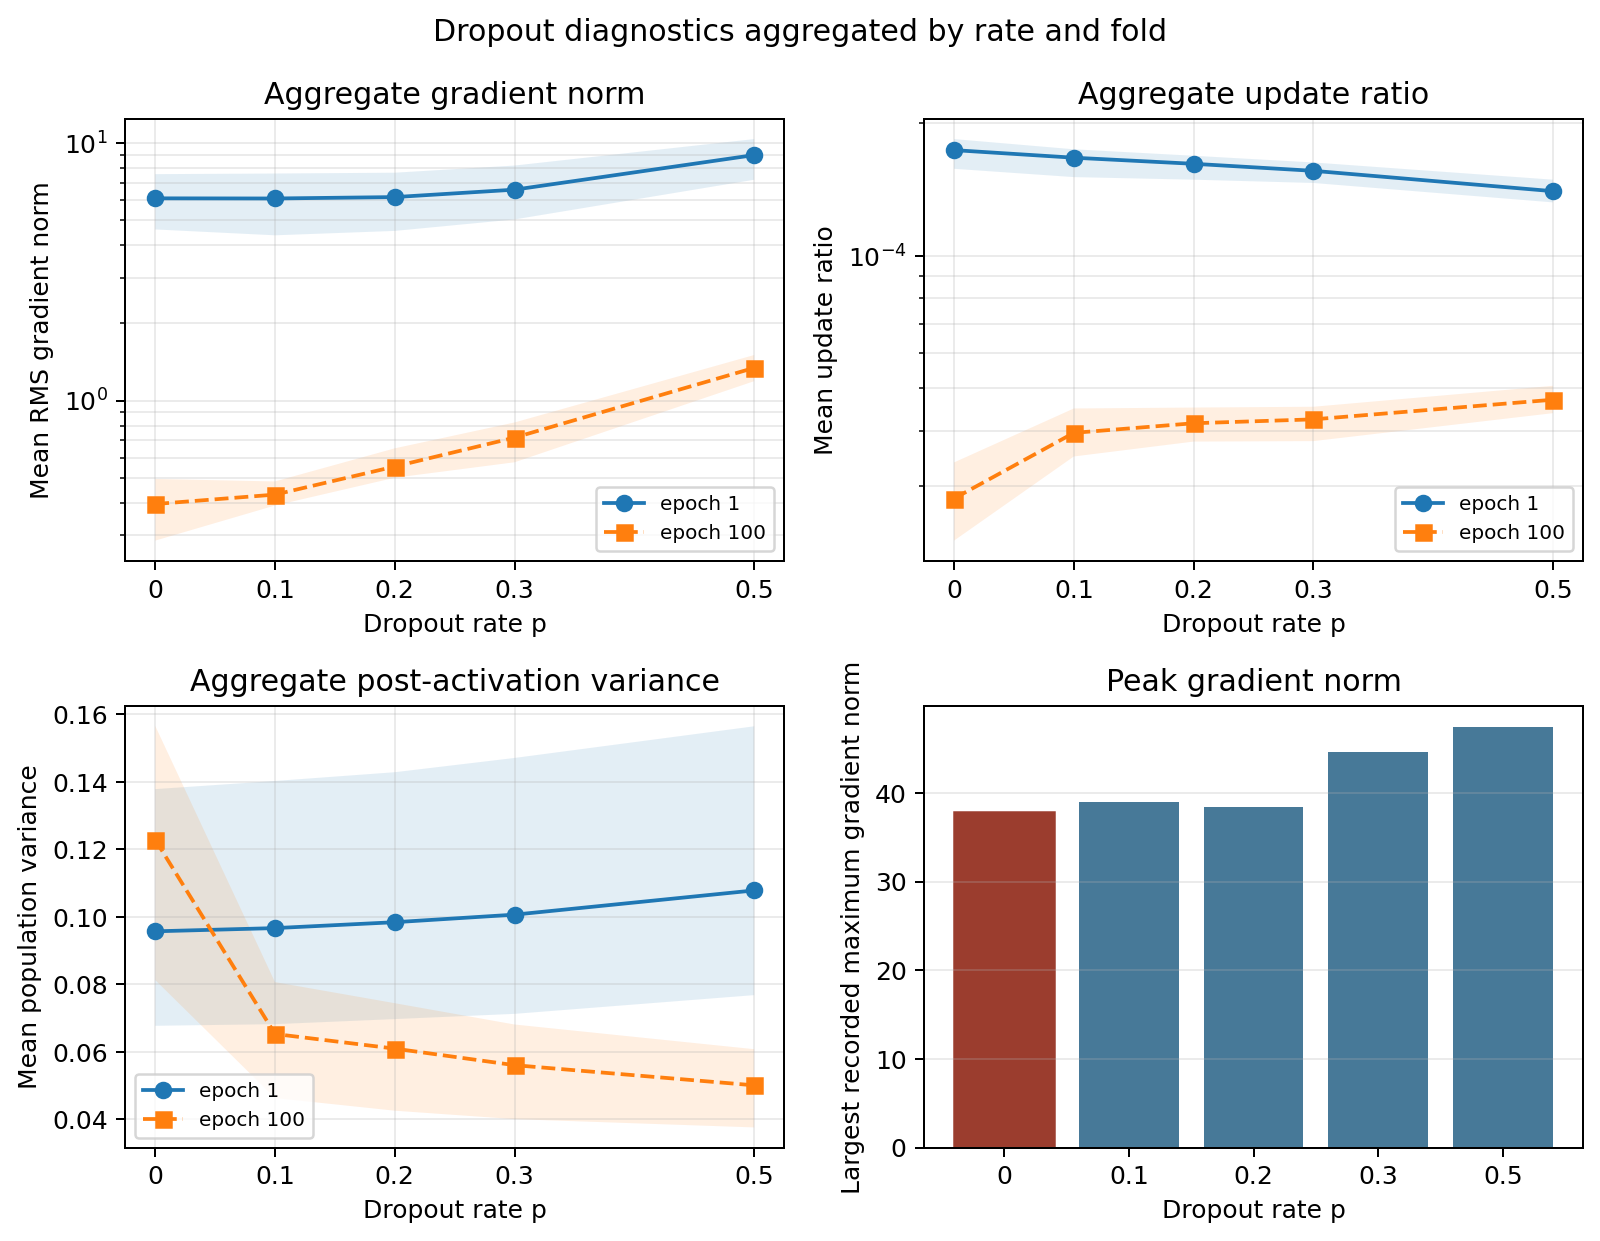
\includegraphics[width=0.95\linewidth]{Images/Chapter04/dropout/dropout_stability.png}
    \caption{Diagnostics for the recorded dropout sweep. The aggregate gradient norm, actual update ratio, and post-activation variance panels show means with minimum to maximum bands over five folds at epochs 1 and 100; the horizontal axis is dropout rate and the first two vertical axes are logarithmic. The final panel shows the largest recorded \texttt{maximum\_norm} with \texttt{parameter\_scope=all} over all folds and epochs for each dropout rate. Diagnostic rows are aggregated and individual layers are not distinguished.}
    \label{fig:04_dropout_stability}
\end{figure}

To understand why dropout degraded performance, we analyzed the detailed training diagnostics, summarized in Figure \ref{fig:04_dropout_stability}. These diagnostics confirm that the poorer performance was not caused by numerical instability but by the disruptive effect of dropout on the optimization process.\\

We can see that no run was numerically unstable. Looking at the bottom right plot, while stronger dropout rates led to larger initial gradient transients (peaking around $47.444652$ for $p=0.5$, compared to $37.841272$ for $p=0.0$), these were controlled, early-epoch events. All gradients remained finite and decreased substantially as training progressed, confirming that the high validation error was not the result of a failed or divergent run.\\

Looking at the other diagnostic panels, late in training, both the average gradient norm and the parameter update ratio systematically increase with the dropout rate. This indicates that dropout forces the optimizer to take larger, more aggressive steps even late in training. However, the post-activation variance shows the opposite trend: at epoch 100, the signal variance decreases as the dropout rate increases. This suggests that while dropout forces larger parameter updates, it may also lead to weaker overall signal propagation through the network.\\

Taken together, these diagnostics paint a clear picture. Dropout did not act as a helpful regularizer; instead, it introduced optimization noise that led to larger, less efficient parameter updates while simultaneously attenuating the network's internal signal. This combination fully explains the degraded validation performance.\\

% The actual parameter movement was small in both cases. For $p=0$, the largest \texttt{mean\_ratio} was $5.0837548\times10^{-4}$. It occurred at zero-based fold 2 and epoch 1 among rows with \texttt{parameter\_scope=all}. The corresponding mean pre-update norm was 15.859737 and the mean update norm was 0.00806269. No row reported a near-zero denominator event. For the weight-only scope, the largest pre-update norm for $p=0$ was 15.878200 at zero-based fold 0, epoch 100, compared with 15.870497 at epoch 1. The largest value for $p=0.5$ was 15.889940, so the poor validation result cannot be attributed to an unbounded parameter norm. The update-ratio curves in Figure~\ref{fig:04_dropout_stability} use the actual before and after parameter values, not the learning rate multiplied by a gradient; they include the optimizer state, clipping, and the current parameter scale.

% Activation statistics give a compatible but limited view of signal propagation. The rows are globally aggregated population statistics; dropout itself does not produce activation statistics, and the recorded post-activation values are measured before the subsequent dropout operation. For $p=0$, the largest post-activation variance over all folds and epochs was 0.186070 at zero-based fold 4 and epoch 100. The corresponding maxima were 0.157550 for $p=0.1$, 0.153652 for $p=0.2$, 0.151285 for $p=0.3$, and 0.185163 for $p=0.5$. These finite values do not establish that dropout caused signal collapse or saturation. The fixed histograms used 64 bins over $[-10,10]$ and placed out-of-range values in the edge bins, so the edge counts were not interpreted as precise tail probabilities. Figure~\ref{fig:04_dropout_stability} aggregates the diagnostic values by dropout rate and shows the peak gradient check for all rates.

Therefore, the cross-validation winner is unequivocally \texttt{dropout rate = 0.0}, with a final validation MSE of $0.005833893\pm0.001006787$. This choice aligns with the default CNN production configuration, which also disables dropout. The evidence from this experiment strongly supports retaining $p=0$ for the final model, as every non-zero rate worsened the paired validation result without providing a meaningful reduction in the already-small overfitting gap.

\subsection{Optimizer tuning}
\label{sec:04_optimizer_tuning}

The optimizer determines how the gradient produced by the SIMM loss is converted into a change of the trainable parameters. For this CNN architecture, this choice is particularly critical: the convolutional feature extractor and the dense regression head differ substantially in parameter dimensions and gradient dynamics. Consequently, a fixed learning rate may lead to different effective progress depending on whether the method retains a direction from previous batches or scales each coordinate using past squared gradients. We decided to test different methods, including vanilla SGD, SGD with momentum, AdaGrad\footnote{That formalizes cumulative coordinate adaptation, as explained by \cite{duchi2011adaptive}.}, RMSprop, and Adam\footnote{That combines first and second moment estimates with bias correction, as seen by \cite{kingma2015adam}.}, to evaluate their impact on the physical validation error within the same finite training budget. The result is a comparison at one learning rate and is not a claim that an optimizer is universally preferable.\\

Before any parameter updates are made, we first apply gradient clipping to prevent numerical instability. In distributed execution, backpropagated gradients are first averaged across all MPI processes via collective reduction (\texttt{MPI\_Allreduce}) to ensure mathematical equivalence regardless of the number of ranks. During early epochs, gradients can become excessively large, especially across wide dense layers. To mitigate this, every individual component of the aggregated gradient vector is constrained to a fixed range. In our implementation, we apply coordinate-wise (component-wise) clipping to each gradient entry $g_{t,j}$ within the interval $[-1,1]$:
\begin{equation}
    \tilde{g}_{t,j}=\operatorname{clip}(g_{t,j},-1,1)
    \label{eq:04_optimizer_clipping}
\end{equation}
This coordinate-wise clipping ensures that no single gradient entry can become disproportionately large, without altering the relative direction of smaller coordinates as a global Euclidean norm clipping ($\tilde{\mathbf{g}}=\mathbf{g}\cdot\min(1,\tau/\lVert\mathbf{g}\rVert_2)$) would. This clipped gradient, $\tilde{g}_{t,j}$, is then handed to the optimizer. No other modifications, such as explicit L1/L2 penalties, are applied to the gradients in this baseline experiment.\\

The five optimizers evaluated in this experiment are defined as follows:
\begin{itemize}
    \item[-] for Vanilla SGD, the update is $$\theta_{t+1,j}=\theta_{t,j}-\eta\tilde{g}_{t,j}$$
    \item[-] for SGD with momentum, the update is defined as 
    \begin{equation*}
    u_{t,j}=\mu u_{t-1,j}+\tilde{g}_{t,j},
    \qquad
    \theta_{t+1,j}=\theta_{t,j}-\eta u_{t,j},
    \qquad \mu=0.9
    \end{equation*}
    \item[-] for AdaGrad, that stores the cumulative squared gradient, the update is defined as 
    \begin{equation*}
    G_{t,j}=G_{t-1,j}+\tilde{g}_{t,j}^{2},
    \qquad
    \theta_{t+1,j}=\theta_{t,j}-
    \frac{\eta\tilde{g}_{t,j}}{\sqrt{G_{t,j}+\varepsilon}},
    \qquad \varepsilon=10^{-8}
    \end{equation*}
    \item[-] for RMSprop, that replaces the cumulative sum with an exponential average, the update is defined as 
    \begin{equation*}
    s_{t,j}=\rho s_{t-1,j}+(1-\rho)\tilde{g}_{t,j}^{2},
    \qquad
    \theta_{t+1,j}=\theta_{t,j}-
    \frac{\eta\tilde{g}_{t,j}}{\sqrt{s_{t,j}+\varepsilon}},
    \qquad \rho=0.9,\quad \varepsilon=10^{-8}
    \end{equation*}
    \item[-] for Adam, that stores both a first moment $m_{t,j}$ and a second moment $v_{t,j}$, the update is defined as 
    \begin{equation*}
    \begin{aligned}
    m_{t,j}&=\beta_1m_{t-1,j}+(1-\beta_1)\tilde{g}_{t,j},
    &v_{t,j}&=\beta_2v_{t-1,j}+(1-\beta_2)\tilde{g}_{t,j}^{2},\\
    \hat{m}_{t,j}&=\frac{m_{t,j}}{1-\beta_1^t},
    &\hat{v}_{t,j}&=\frac{v_{t,j}}{1-\beta_2^t},\\
    \theta_{t+1,j}&=\theta_{t,j}-\eta
    \frac{\hat{m}_{t,j}}{\sqrt{\hat{v}_{t,j}}+\varepsilon},
    &\beta_1&=0.9,\quad \beta_2=0.999,\quad \varepsilon=10^{-8}
    \end{aligned}
    \end{equation*}
\end{itemize}
In all five algorithms, the baseline learning rate is set to $\eta=10^{-5}$ without an attached decay scheduler.\\

In our \cpp framework, each candidate optimizer is encapsulated as an \texttt{OptimizerRecipe} (e.g., \texttt{Recipes::adam}, \texttt{Recipes::rmsprop}). When \texttt{CrossValidator} evaluates a fold, a fresh optimizer instance is constructed. For stateful optimizers, parameter state vectors ($m_t, v_t, s_t, G_t$) are zero-initialized and bound to weight arrays via an internal pointer hash map (\texttt{std::unordered\_map<float*, State>}), ensuring strict fold isolation with $\mathcal{O}(1)$ lookup complexity and zero cross-fold state leakage. Although Adam triples the parameter memory requirement (storing two additional 32-bit floats per parameter, approximately $96\,\mathrm{MB}$ for our $\approx 8.065\times 10^6$ parameter network), this overhead is easily accommodated by system memory.\\

The optimizer comparison was performed exactly in the same way that the dropout one was done, using the winning topology from Section \ref{sec:04_topology_tuning} and the same cross-validation protocol. All other hyperparameters were held constant: SIMM physics weight of $0.25$, batch size of 64, and a 100-epoch training budget.\\

The winning optimizer was selected based on the lowest physical-unit validation MSE (Equation \eqref{eq:04_validation_mse}). The final scores reported in Table \ref{tab:04_optimizer_results} are the sample-weighted averages across the five folds, ensuring that folds with slightly different numbers of validation samples are handled correctly. The results, as shown in Figure \ref{fig:04_optimizer_ranking}, demonstrate a clear performance hierarchy among the tested optimizers.\\

Adam was the cross-validation winner with $0.004426734\pm0.000793966$ physical validation MSE. It was the lowest-scoring candidate in every one of the five cross-validation folds. This represents a significant $15\%$ error reduction compared to its closest competitor, RMSprop (MSE of $0.005216$), and a $38\%$ reduction compared to SGD with momentum. The other optimizers ranked as expected, with AdaGrad and momentum-based SGD delivering intermediate performance. Vanilla SGD, without any adaptive or momentum mechanisms, struggled significantly at this low learning rate, finishing with a validation error nearly four times higher than Adam's ($0.017924$). While all runs completed successfully without diverging, the performance of plain SGD was substantially less accurate and consistent across the folds.\\

\begin{table}[htbp]
    \centering
    \small
    \setlength{\tabcolsep}{3pt}
    \begin{tabularx}{\linewidth}{@{}
        >{\raggedright\arraybackslash}X
        >{\centering\arraybackslash}X
        >{\centering\arraybackslash}X
        >{\centering\arraybackslash}X
        >{\centering\arraybackslash}X
        @{}}
        \hline
        Optimizer &
        Mean validation MSE &
        Fold standard deviation &
        Minimum fold &
        Maximum fold \\
        \hline
        Adam & 0.004427 & 0.000794 & 0.002879 & 0.005044 \\
        RMSprop & 0.005216 & 0.000585 & 0.004518 & 0.006173 \\
        AdaGrad & 0.006184 & 0.001108 & 0.004239 & 0.007439 \\
        SGD + momentum & 0.007150 & 0.001264 & 0.004791 & 0.008473 \\
        SGD & 0.017924 & 0.005568 & 0.013063 & 0.028647 \\
        \hline
    \end{tabularx}
    \caption{Complete optimizer comparison at learning rate $10^{-5}$. The means and fold deviations are sample-weighted physical validation MSE values, with the deviation defined as the weighted population standard deviation over the five folds. The minimum and maximum columns show the corresponding unweighted extrema of the fold scores.}
    \label{tab:04_optimizer_results}
\end{table}

The physical training MSE recorded after the final fold epoch was also lower for the better validation candidates, but it must be interpreted separately from the SIMM objective: the methods that achieved better validation scores also reached a lower physical training MSE within the fixed 100-epoch training budget.\\

\begin{figure}[H]
    \centering
    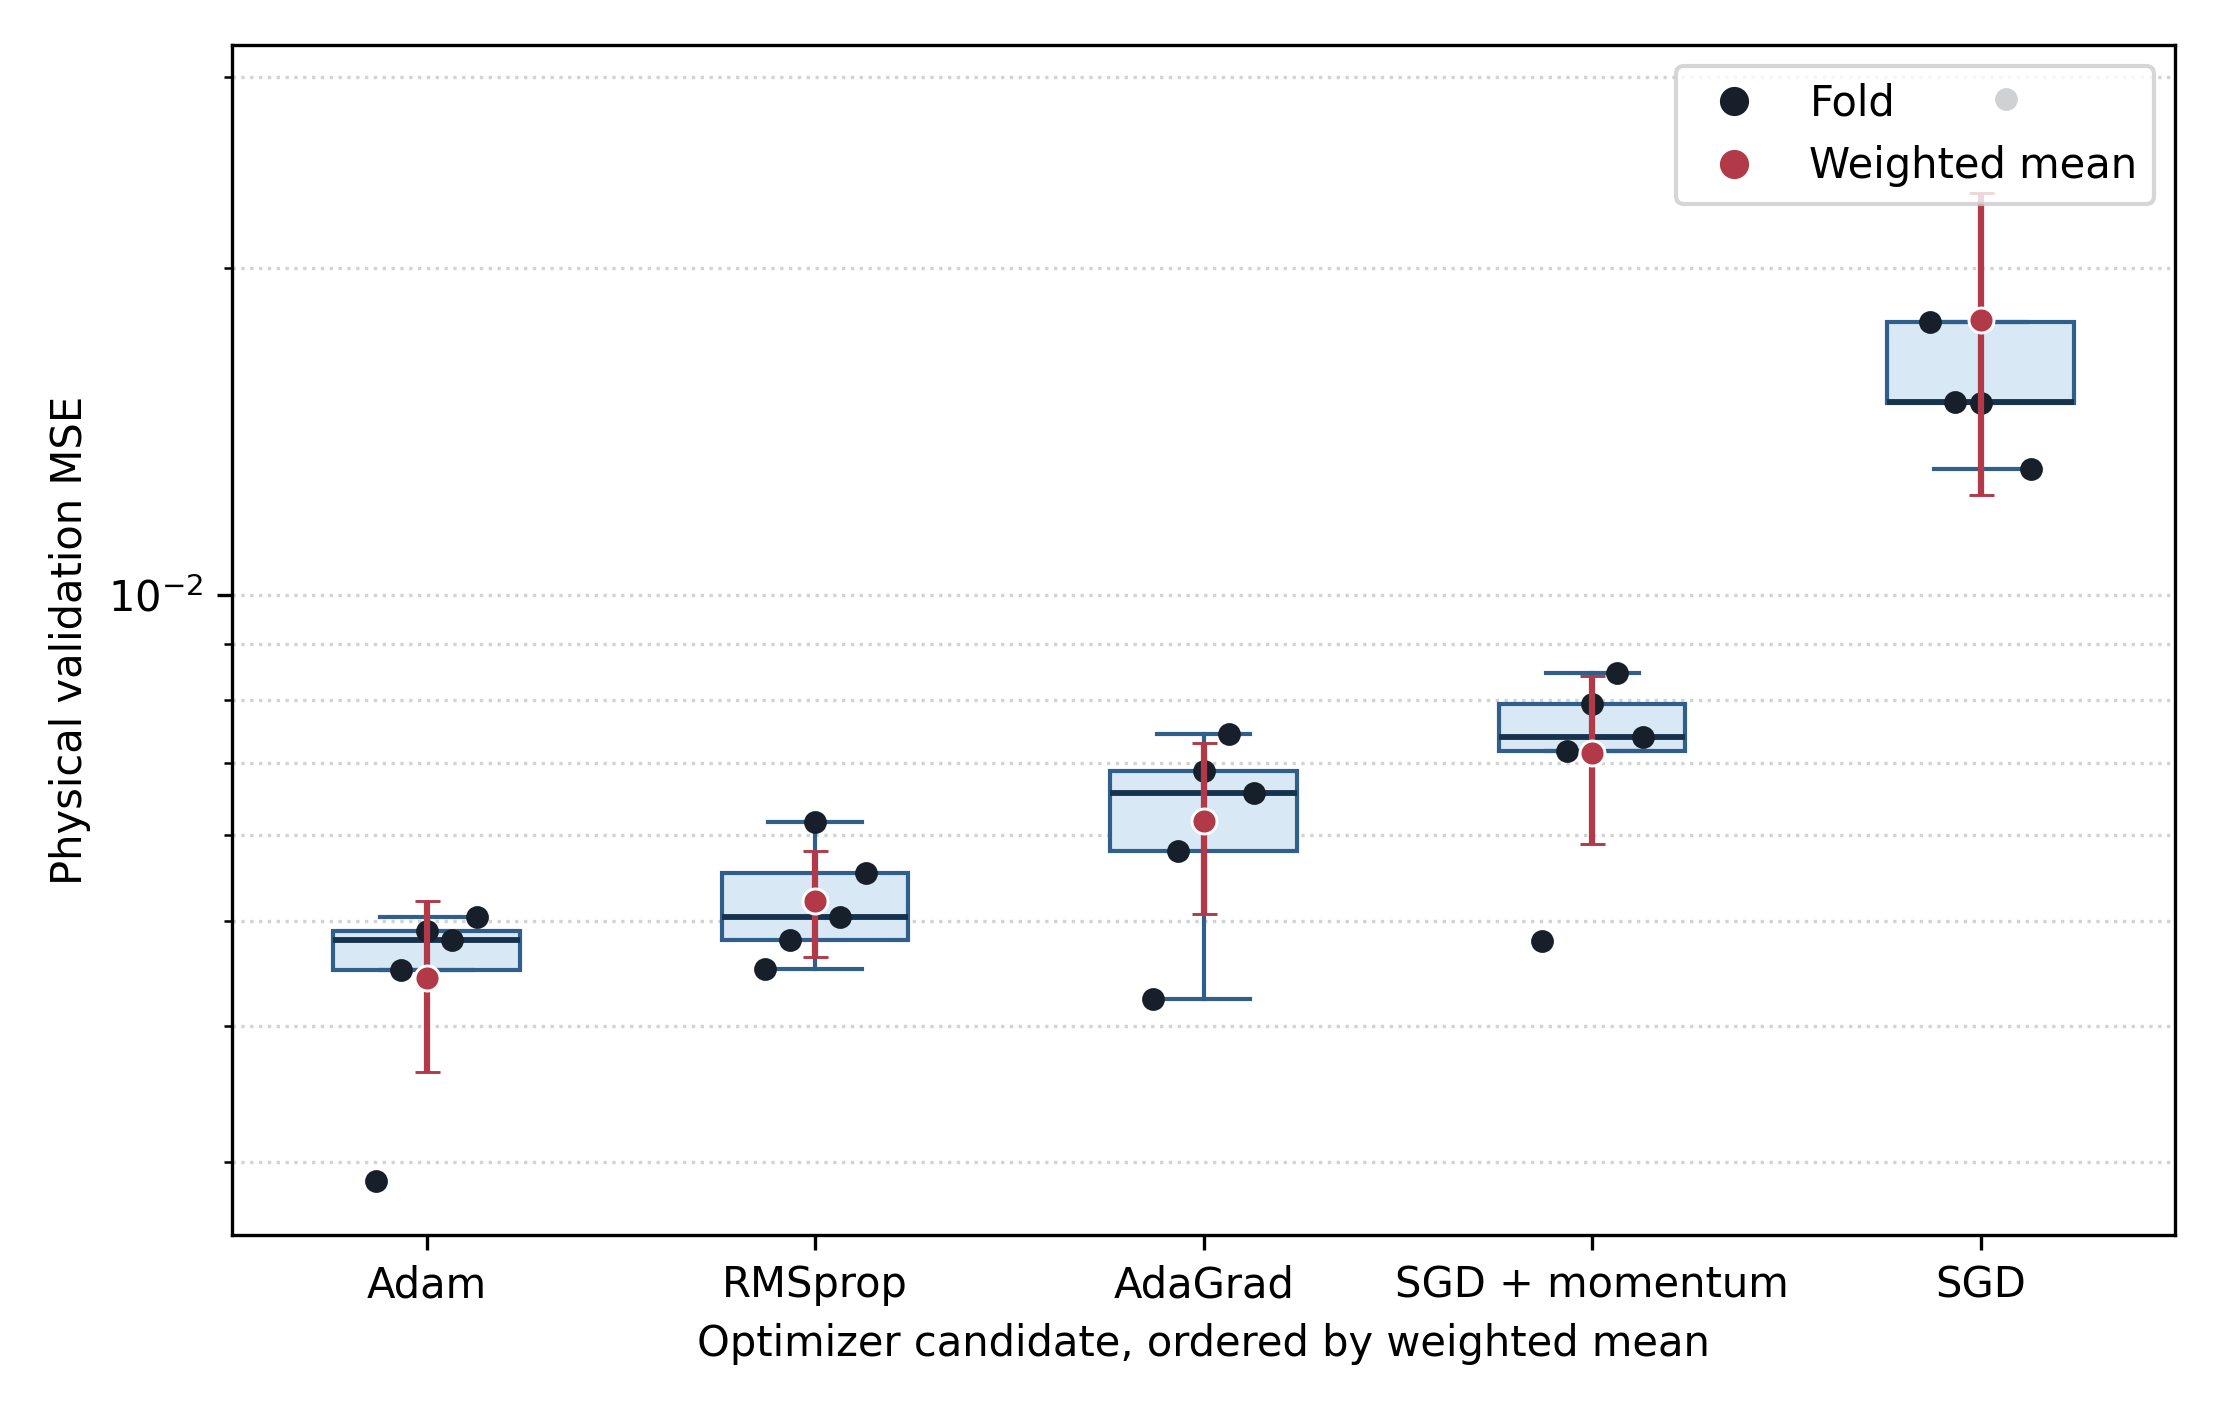
\includegraphics[width=0.80\linewidth]{Images/Chapter04/optimizer/optimizer_ranking.png}
    \caption{Optimizer ranking from the five-fold comparison at learning rate $10^{-5}$. Dark points are individual physical validation MSE values, boxes summarize the five folds, and red points with bars show the sample-weighted mean and weighted population standard deviation. The vertical axis is logarithmic.}
    \label{fig:04_optimizer_ranking}
\end{figure}

The training histories, visualized in Figure \ref{fig:04_optimizer_history}, provide a clear explanation for the final performance ranking by showing how each optimizer converged over the 100-epoch budget.\\

The superiority of the adaptive coordinate methods is evident from the very beginning. Adam and RMSprop immediately establish a lead, starting with and maintaining a significantly lower validation error than the other candidates. However, the plot also highlights key algorithmic distinctions:
\begin{itemize}
    \item[-] AdaGrad accumulates the sum of all past squared gradients $G_{t,j}=\sum_{\tau=1}^t \tilde{g}_{\tau,j}^2$. Because this denominator grows monotonically, the effective learning rate diminishes as $\mathcal{O}(1/\sqrt{t})$. Consequently, AdaGrad prematurely stalls in later epochs and cannot escape shallow local sub-optima;
    \item[-] RMSprop resolves AdaGrad's diminishing step size by replacing the monotonic sum with an exponentially decaying average ($\rho=0.9$). However, it lacks first-moment momentum and initialization bias correction. Without momentum to filter high-frequency gradient jitter, RMSprop exhibits notable instability late in training, with its error spiking noticeably around epoch 90 before recovering;
    \item[-] Plain SGD and SGD with momentum scale parameter updates directly by the unnormalized gradient magnitude ($\lVert\Delta\theta\rVert\approx\eta\lVert\tilde{g}\rVert$). As backpropagated gradients naturally decay near flatter loss regions, the effective step size becomes vanishingly small ($\approx 10^{-7}$--$10^{-8}$ for $\eta=10^{-5}$), preventing SGD from covering sufficient distance across the loss landscape within 100 epochs. In contrast, Adam's coordinate normalization by $\sqrt{\hat{v}_{t,j}}$ maintains active effective steps of scale $\eta$ across all coordinates regardless of gradient magnitude decay.
\end{itemize}
\vspace{2ex}

\begin{figure}[H]
    \centering
    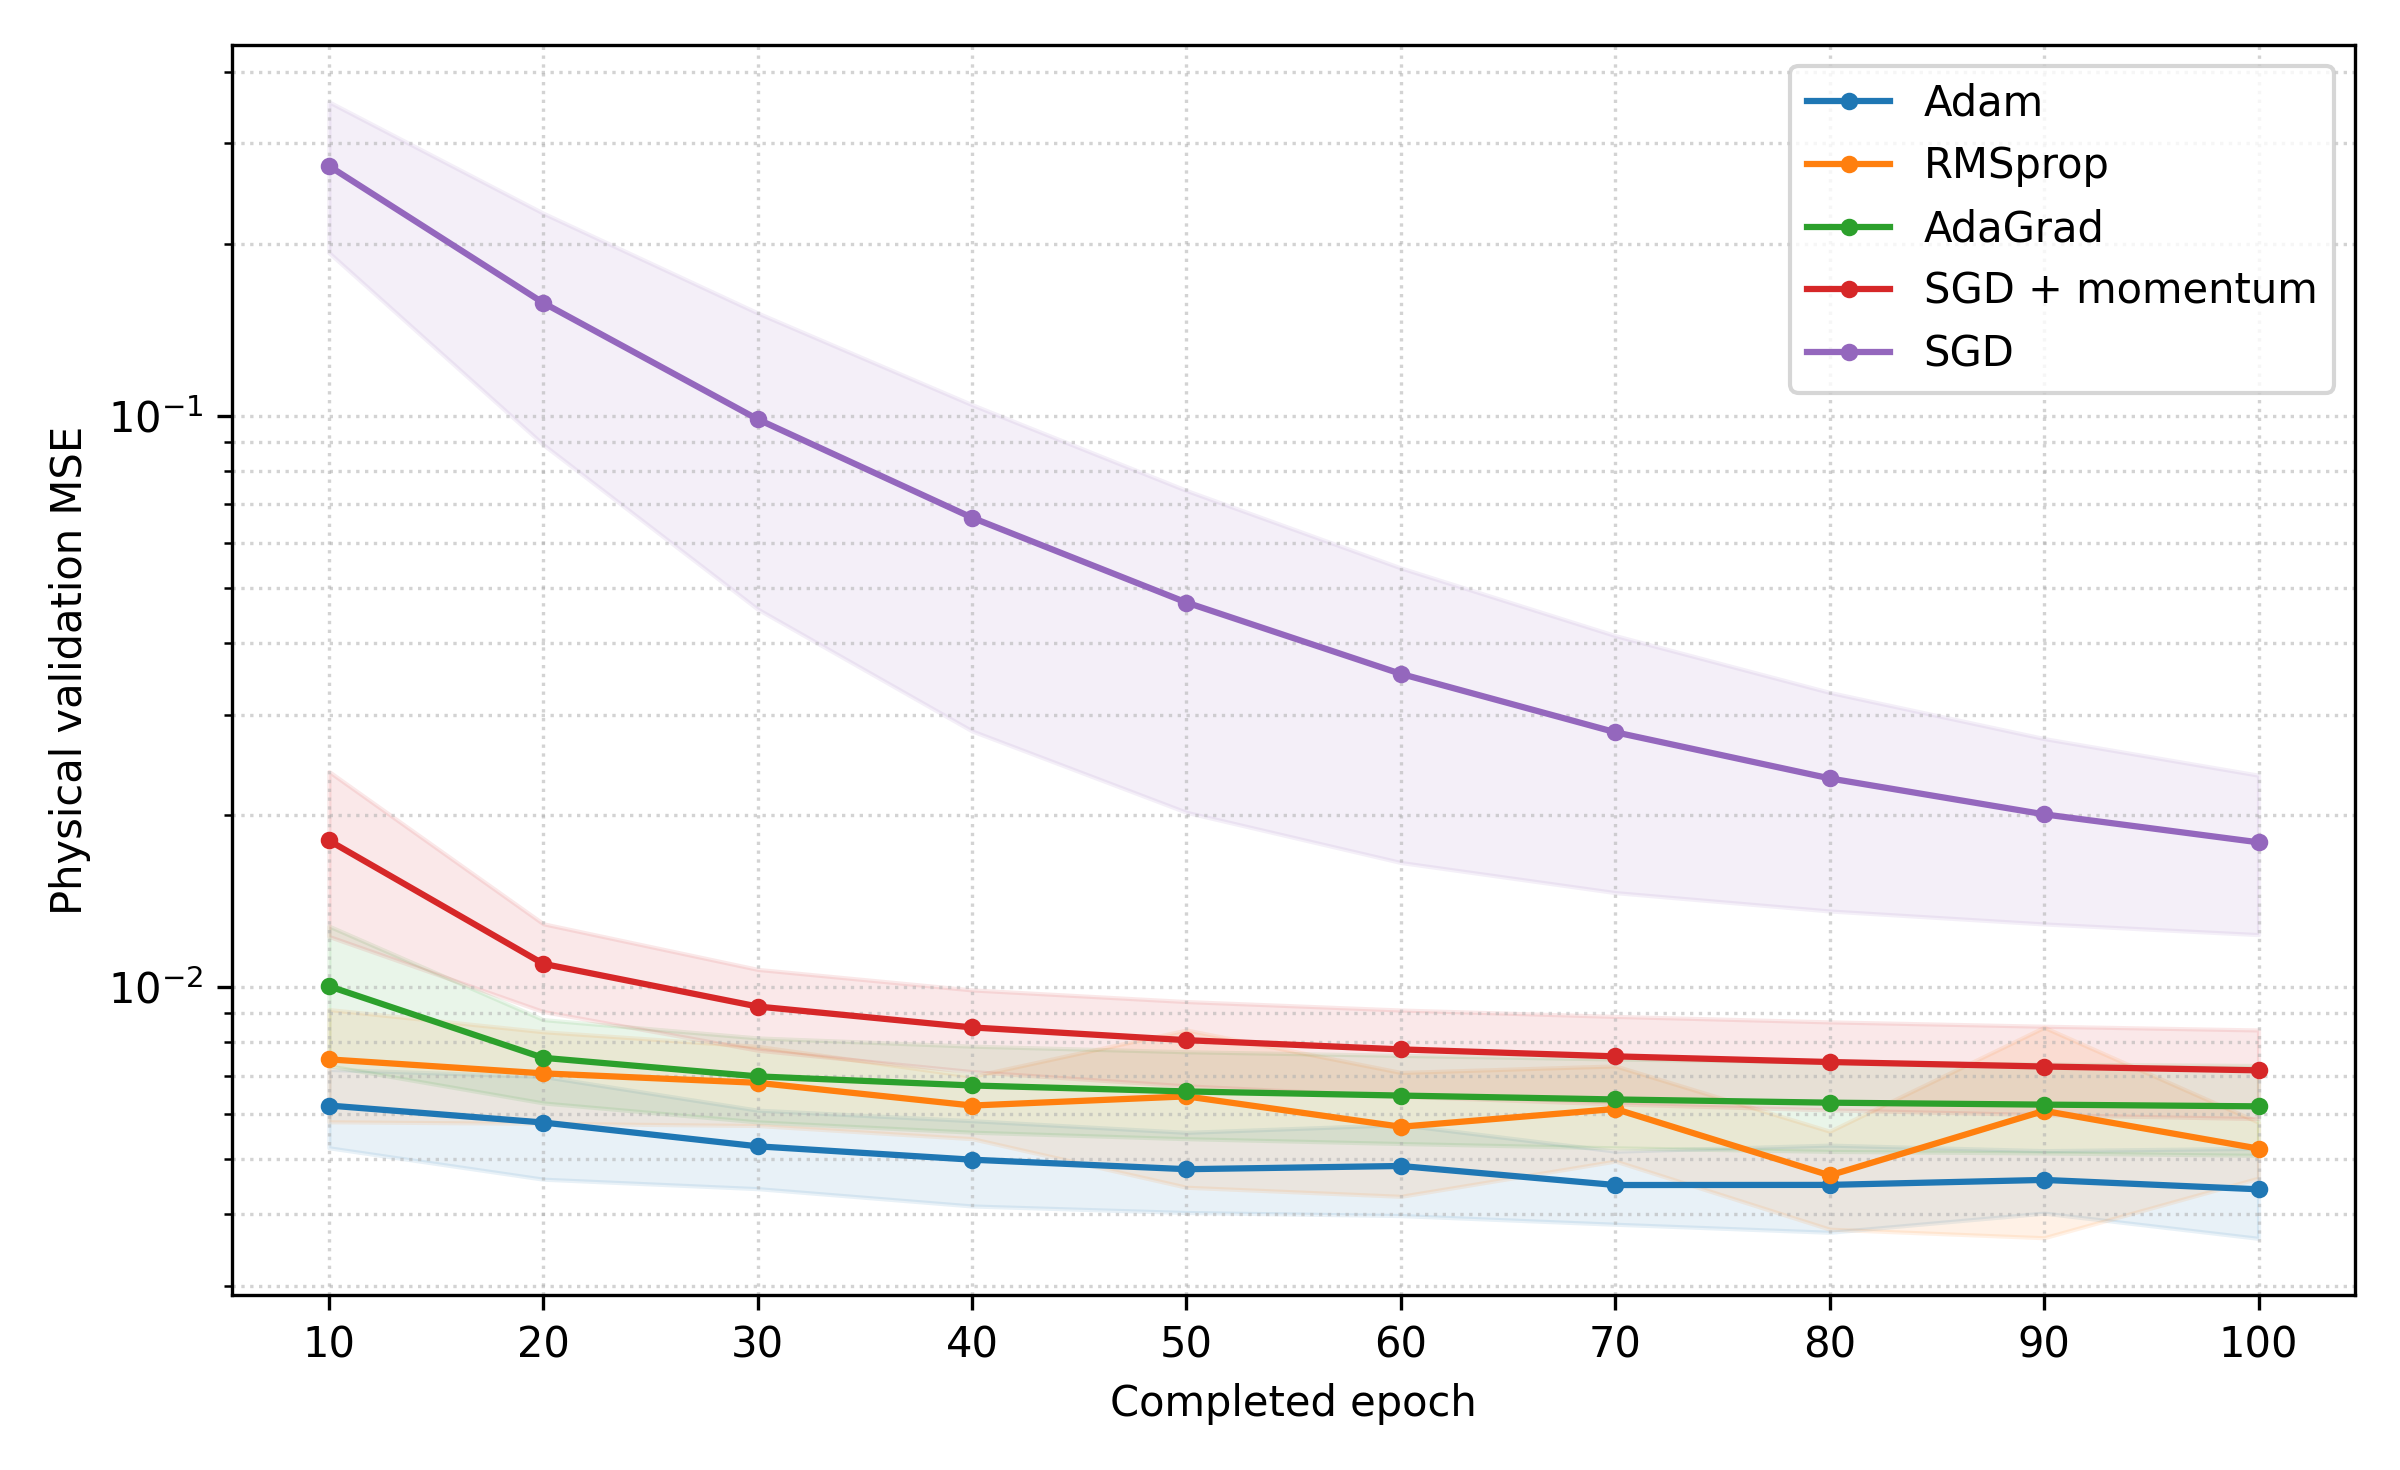
\includegraphics[width=0.80\linewidth]{Images/Chapter04/optimizer/optimizer_history.png}
    \caption{Physical validation MSE at the ten-epoch history checkpoints for the five optimizer candidates. Lines and shaded regions are the sample-weighted means and weighted population standard deviations over the five folds. The vertical axis is logarithmic; the SIMM training objective and the test set are not shown.}
    \label{fig:04_optimizer_history}
\end{figure}

Overall, the convergence plot visually confirms the final rankings. It demonstrates that Adam's victory is due not only to a lower final error but also to its combination of fast, efficient, and stable convergence throughout the entire training process.\\

The diagnostic plots for the winning Adam optimizer reveal why it was so much more effective and stable than the alternatives. The key architectural challenge is visualized in Figure \ref{fig:04_optimizer_gradient_magnitude}, which plots the gradient magnitudes for each trainable layer at different points in training.\\

The plot shows a massive initial gradient peak at layer index $4$, which corresponds to the first dense layer (\texttt{DenseLayer(7202, 1024)}). This single layer contains $7{,}375{,}872$ parameters (weights and biases), accounting for over $91.4\%$ of the total $8{,}065{,}025$ parameters in the network. At epoch 1, the gradients in this layer are an order of magnitude larger than in any other layer. This transient gradient concentration occurs when the spatial features from the convolutional trunk ($30\times 30\times 8 = 7200$ features plus two flow scalars) are projected into the wide dense head. Adam is uniquely suited to handle this dimension bottleneck: coordinate-adaptive scaling ($\sqrt{\hat{v}_{t,j}}+\varepsilon$) normalizes the effective step size per coordinate, preventing the massive dense layer from overpowering the convolutional kernels or destabilizing the network. In contrast, unscaled methods like SGD apply the same uniform scaling to both small convolutional kernels and massive dense layers, leading to severe under-stepping in some layers and oscillation in others.\\

The plot also shows that by epoch 10, Adam has successfully navigated this transient phase. The gradients across all layers have settled into a much more stable and well-behaved pattern, allowing for smooth convergence for the rest of training. This successful management of the network's challenging gradient landscape is a primary reason for Adam's superior efficiency and stability.\\

\begin{figure}[H]
    \centering
    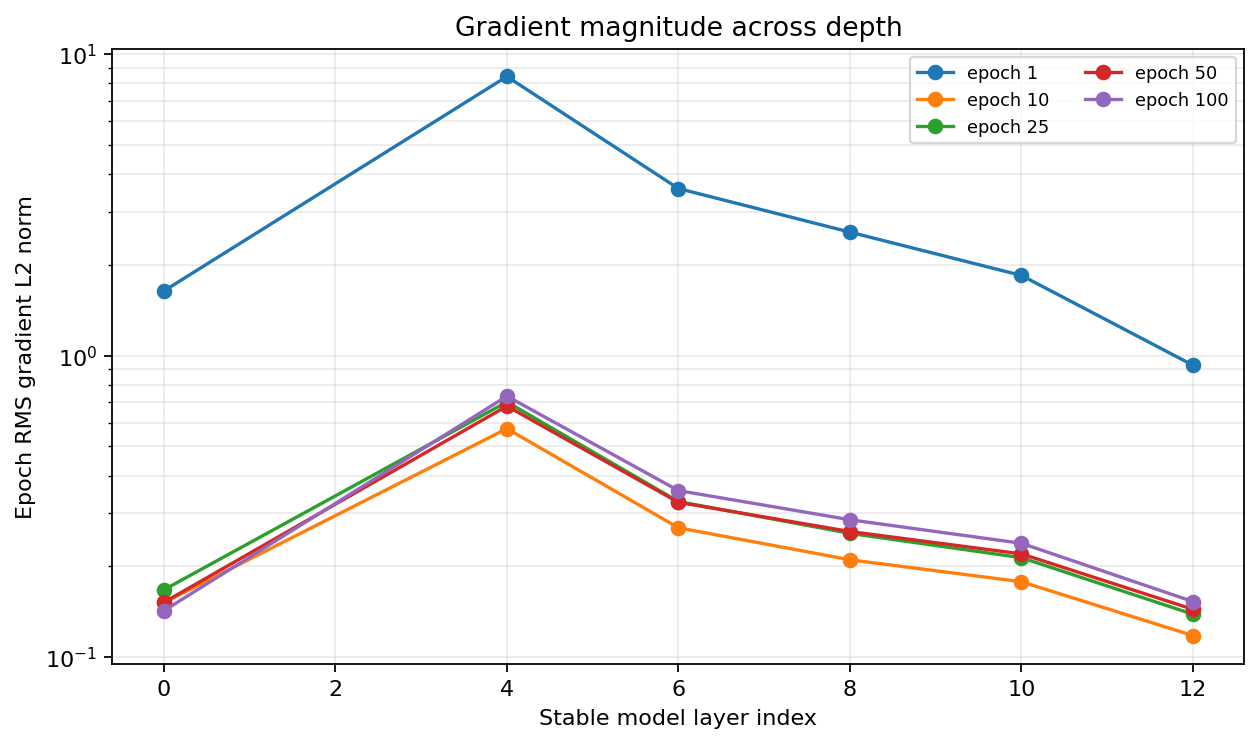
\includegraphics[width=0.8\linewidth]{Images/Chapter04/optimizer/optimizer_gradient.png}
    \caption{The RMS gradient norm for each trainable layer, plotted at different training epochs. The vertical axis is logarithmic. The plot reveals a massive gradient peak in the first dense layer (index 4) at the start of training (epoch 1). This initial transient is rapidly stabilized by the Adam optimizer, with gradient magnitudes becoming substantially smaller and more uniform across the network's depth by epoch 10.}
    \label{fig:04_optimizer_gradient_magnitude}
\end{figure}

The cross-validation experiment identified Adam as the decisively superior optimizer for this task, outperforming all competitors in every fold. The diagnostic analysis confirms that its stability and efficiency stem from its ability to handle the large and varied gradient magnitudes that arise naturally from the network's convolutional-to-dense architecture. The final refit of this experimental winner on the full training set yielded a test MSE of $0.003655$.

\subsection{Physics-weight tuning}
\label{sec:04_physics_weight_tuning}

The SIMM term was tuned because it is the only part of the objective that encodes an aerodynamic relation not learned directly from the CFD targets. A positive physics weight can improve the low-angle regime if the thin-airfoil relation supplies useful information, but it can also pull the prediction away from the simulation data when the relation is only approximate. The experiment therefore asks whether the prior improves the physical-unit validation error, rather than assuming that a larger physics contribution is beneficial. The search was performed over the training dataset only and the untouched test dataset was not used to choose the weight.\\

The implementation evaluates the loss in the fold-specific standardized target space. Let $C_{L,i}$ be the physical target, let $\mu_y$ and $s_y$ be the target mean and standard deviation fitted on the training part of a fold, and let $a_i$ be the angle of attack in radians. The standardized target and prediction are $y_i=(C_{L,i}-\mu_y)/s_y$ and $\hat{y}_i$, while the standardized physical target is:
\begin{equation}
    y_i^{\mathrm{phys}}=\frac{2\pi a_i-\mu_y}{s_y}
    \label{eq:04_physics_target}
\end{equation}
The mask is evaluated on the unstandardized angle,
\begin{equation}
    M_i=\begin{cases}
        1, & |a_i|\leq 0.174533\ \mathrm{rad}\\
        0, & |a_i|>0.174533\ \mathrm{rad}
    \end{cases}
    \label{eq:04_physics_mask}
\end{equation}
which corresponds to $|\alpha|\leq10^\circ$. The actual batch objective is:
\begin{equation}
    \mathcal{L}=\frac{1}{N}\sum_{i=1}^{N}(\widehat{y}_i-y_i)^2
    +\lambda\frac{1}{N}\sum_{i=1}^{N}M_i
    (\widehat{y}_i-y_i^{\mathrm{phys}})^2,
    \label{eq:04_simm_loss}
\end{equation}
where the physics sum is divided by the full batch size, not by the number of masked samples. The prediction gradient used by backpropagation is consequently
\begin{equation}
    \frac{\partial\mathcal{L}}{\partial\widehat{y}_i}
    =\frac{2}{N}\left[(\widehat{y}_i-y_i)
    +\lambda M_i(\widehat{y}_i-y_i^{\mathrm{phys}})\right].
    \label{eq:04_physics_gradient}
\end{equation}
The validation score is converted back to physical units by multiplying the standardized prediction residual by $s_y$ before squaring. Therefore, the SIMM objective and the selection metric have different units and cannot be ranked by their numerical magnitudes.\\

To determine the optimal strength of the physical term, we performed a sweep over seven different values for the physics weight $\lambda\in\{0,0.05,0.1,0.25,0.5,1,2\}$. The baseline case, $\lambda=0.0$, corresponds to a purely data-driven model without any physics-informed loss.\\

As in the other tuning, all other hyperparameters were held constant, including the winning topology from Section \ref{sec:04_topology_tuning}, the Adam optimizer with a learning rate of $10^{-5}$, a batch size of 64, and a 100-epoch training budget. In the codebase, the physics loss strength $\lambda$ is configured through the \texttt{LossConfig} structure and \texttt{Trainer} computes the masked analytical thin-airfoil penalty on the standardized predictions at each forward pass. The cross-validation protocol was identical to the previous experiments, ensuring that the only variable was the physics weight $\lambda$.\\

The results of the sweep, summarized in Table \ref{tab:04_physics_results}, lead to a clear conclusion: the physics-informed loss term did not improve the model's predictive accuracy.

\begin{table}[h!]
    \centering
    \begin{tabular}{rccrr}
        \hline
        $\lambda$ & Mean validation MSE & Fold standard deviation & $\Delta_{\lambda}$ & Improved folds \\
        \hline
        0.00 & 0.005600634 & 0.001099091 & 0 & -- \\
        0.05 & 0.005637647 & 0.001136246 & +0.000037038 & 1/5 \\
        0.10 & 0.005629100 & 0.001116111 & +0.000028457 & 1/5 \\
        0.25 & 0.005706661 & 0.001195944 & +0.000106089 & 1/5 \\
        0.50 & 0.006025918 & 0.001193569 & +0.000425322 & 0/5 \\
        1.00 & 0.006581512 & 0.001350790 & +0.000981093 & 0/5 \\
        2.00 & 0.007406998 & 0.001519330 & +0.001806727 & 0/5 \\
        \hline
    \end{tabular}
    \caption{Recorded physics-weight sweep. The mean and deviation are the sample-weighted physical validation values in \texttt{cv\_summary.csv}. $\Delta_{\lambda}$ is the paired candidate minus reference validation MSE, so positive values are worse than $\lambda=0$.}
    \label{tab:04_physics_results}
\end{table}

The best performance was achieved by the purely data-driven model ($\lambda=0$), which recorded a mean validation MSE of $0.005600634\pm0.001099091$. As shown in the performance plot (Figure \ref{fig:04_physics_performance}, left panel), every non-zero value of $\lambda$ resulted in a higher validation error. While the degradation was minimal for small weights like $\lambda=0.05$, performance grew progressively worse as the physics term was given more influence.\\

\begin{figure}[H]
    \centering
    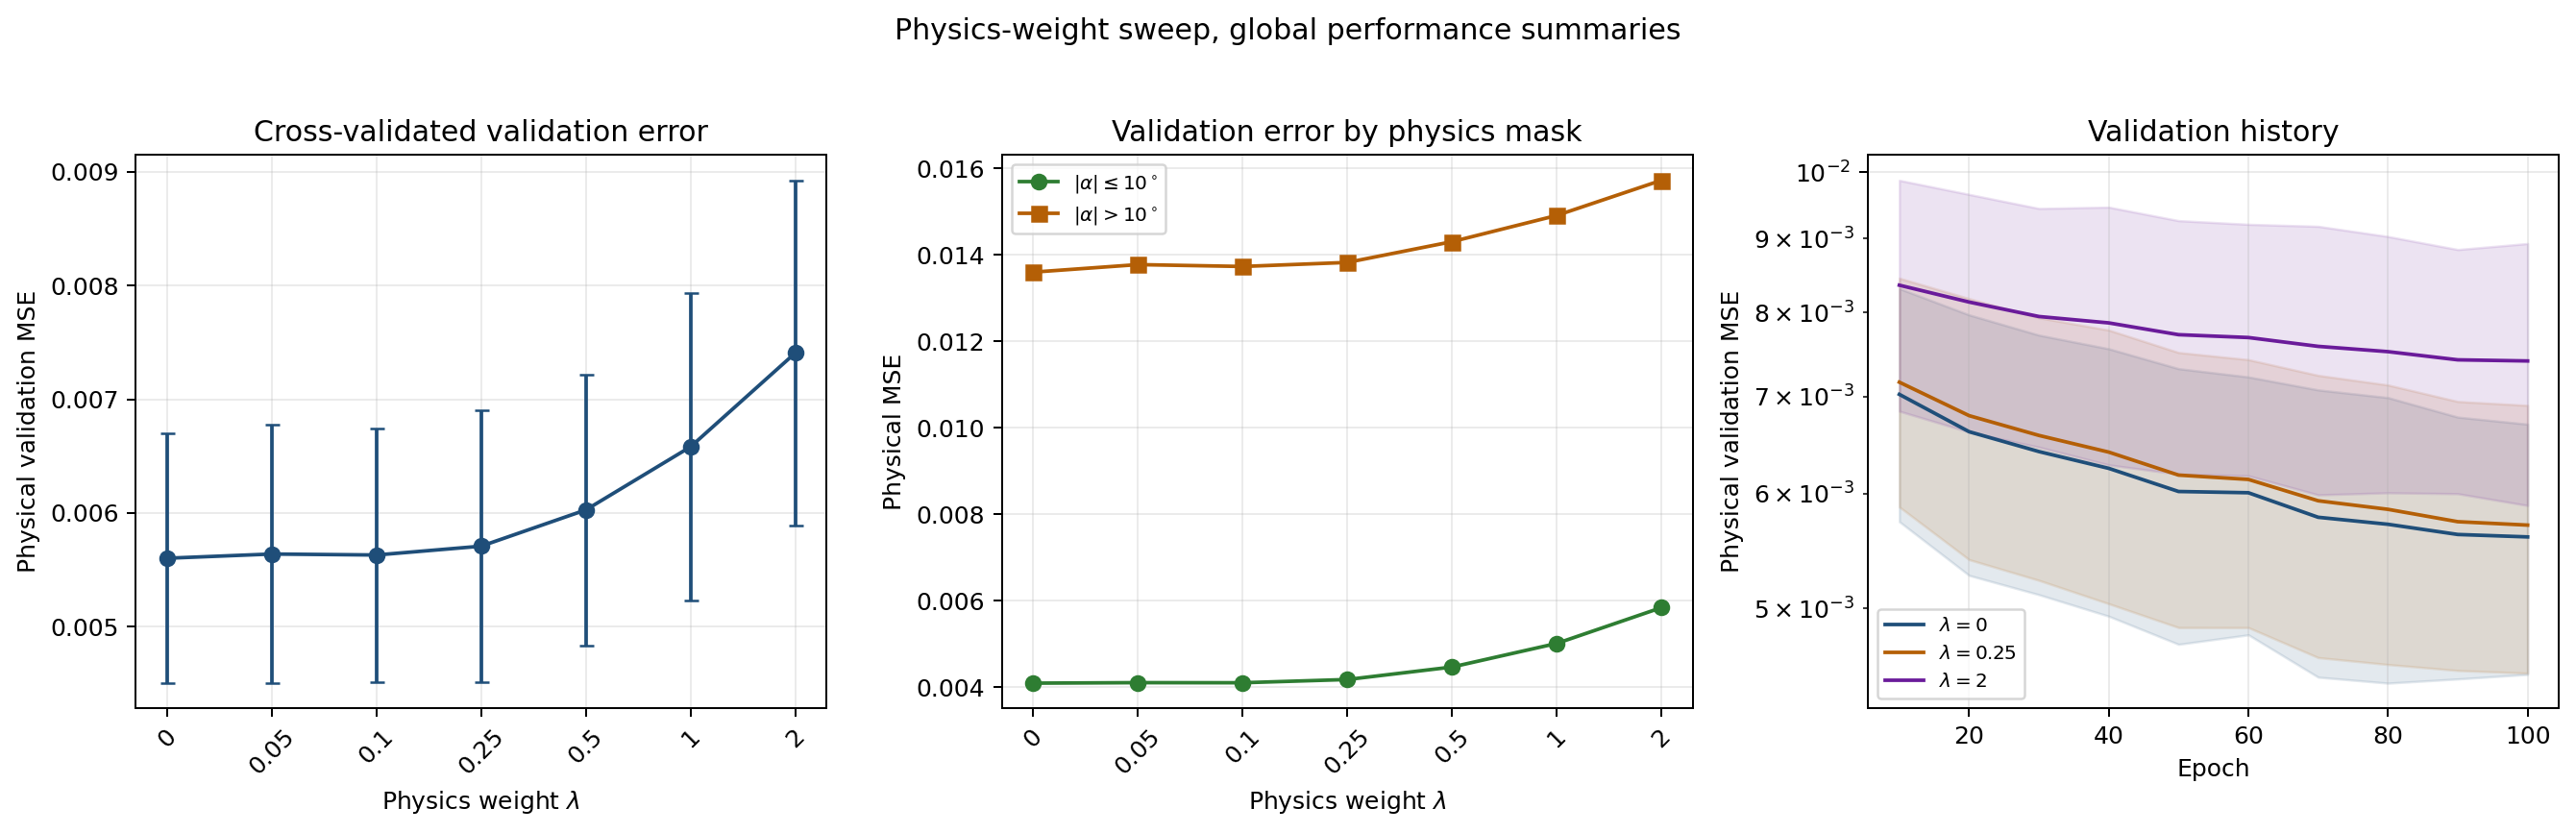
\includegraphics[width=0.98\linewidth]{Images/Chapter04/physics/physics_performance.png}
    \caption{Global summaries of the recorded physics-weight sweep. The first panel shows sample-weighted mean physical validation MSE with fold deviations, the second separates the count-weighted low-angle and high-angle validation errors, and the third shows physical validation histories for $\lambda=0$, $0.25$, and $2$ with fold-spread bands. The training SIMM objective is not placed on the validation-MSE axis.}
    \label{fig:04_physics_performance}
\end{figure}

To investigate this further, we tested whether the physics term provided a localized benefit in the low-angle-of-attack regime where its underlying theory is valid. We split the validation data into low-angle ($|\alpha|\leq10^\circ$) and high-angle ($|\alpha|>10^\circ$) groups, respectively with a count of 1442 and 271 samples across the five folds. The results of this split are shown in the second panel of Figure \ref{fig:04_physics_performance} (middle panel), are decisive. For $\lambda=0$, the count-weighted MSE was $0.004096627$ in the low-angle group and $0.013603506$ in the high-angle group. At $\lambda=2$, the corresponding values were $0.005843330$ and $0.015727326$. Both groups therefore worsened as the prior became strong; the effect was not a selective improvement in the masked regime.\\

The validation history is consistent with the final ranking. The fold-averaged validation MSE for $\lambda=0$ decreased from approximately $0.007025$ at epoch 10 to $0.005602$ at epoch 100, whereas the corresponding values for $\lambda=2$ were $0.008356$ and $0.007407$. Every candidate completed 100 epochs with finite values, converging to a stable solution. The training objective started and ended higher as $\lambda$ increased, from approximately $0.599$ to $0.0104$ for $\lambda=0$ and from $1.393$ to $0.0168$ for $\lambda=2$ when averaged over folds. These are standardized SIMM objectives, so their difference from the physical validation MSE is not a generalization gap.\\

The diagnostic plots in Figure \ref{fig:04_physics_diagnostics} show that the optimizer successfully managed the training process for all candidates. As seen in the left panel, strengthening the physics prior led to a more pronounced initial gradient transient. At epoch 1, the aggregate RMS gradient norm for the $\lambda=2$ model (mean of $45.36$) was more than double that of the purely data-driven model ($\lambda=0$, mean of $18.76$). However, this was a controlled, early-epoch event. The optimizer rapidly stabilized all runs, and by epoch 100, the aggregate gradient norms had settled to a much smaller and more comparable level ($0.842$ for $\lambda=0$ vs. $1.071$ for $\lambda=2$). This pattern confirms that the training was numerically stable and did not suffer from late-stage exploding gradients.\\

\begin{figure}[H]
    \centering
    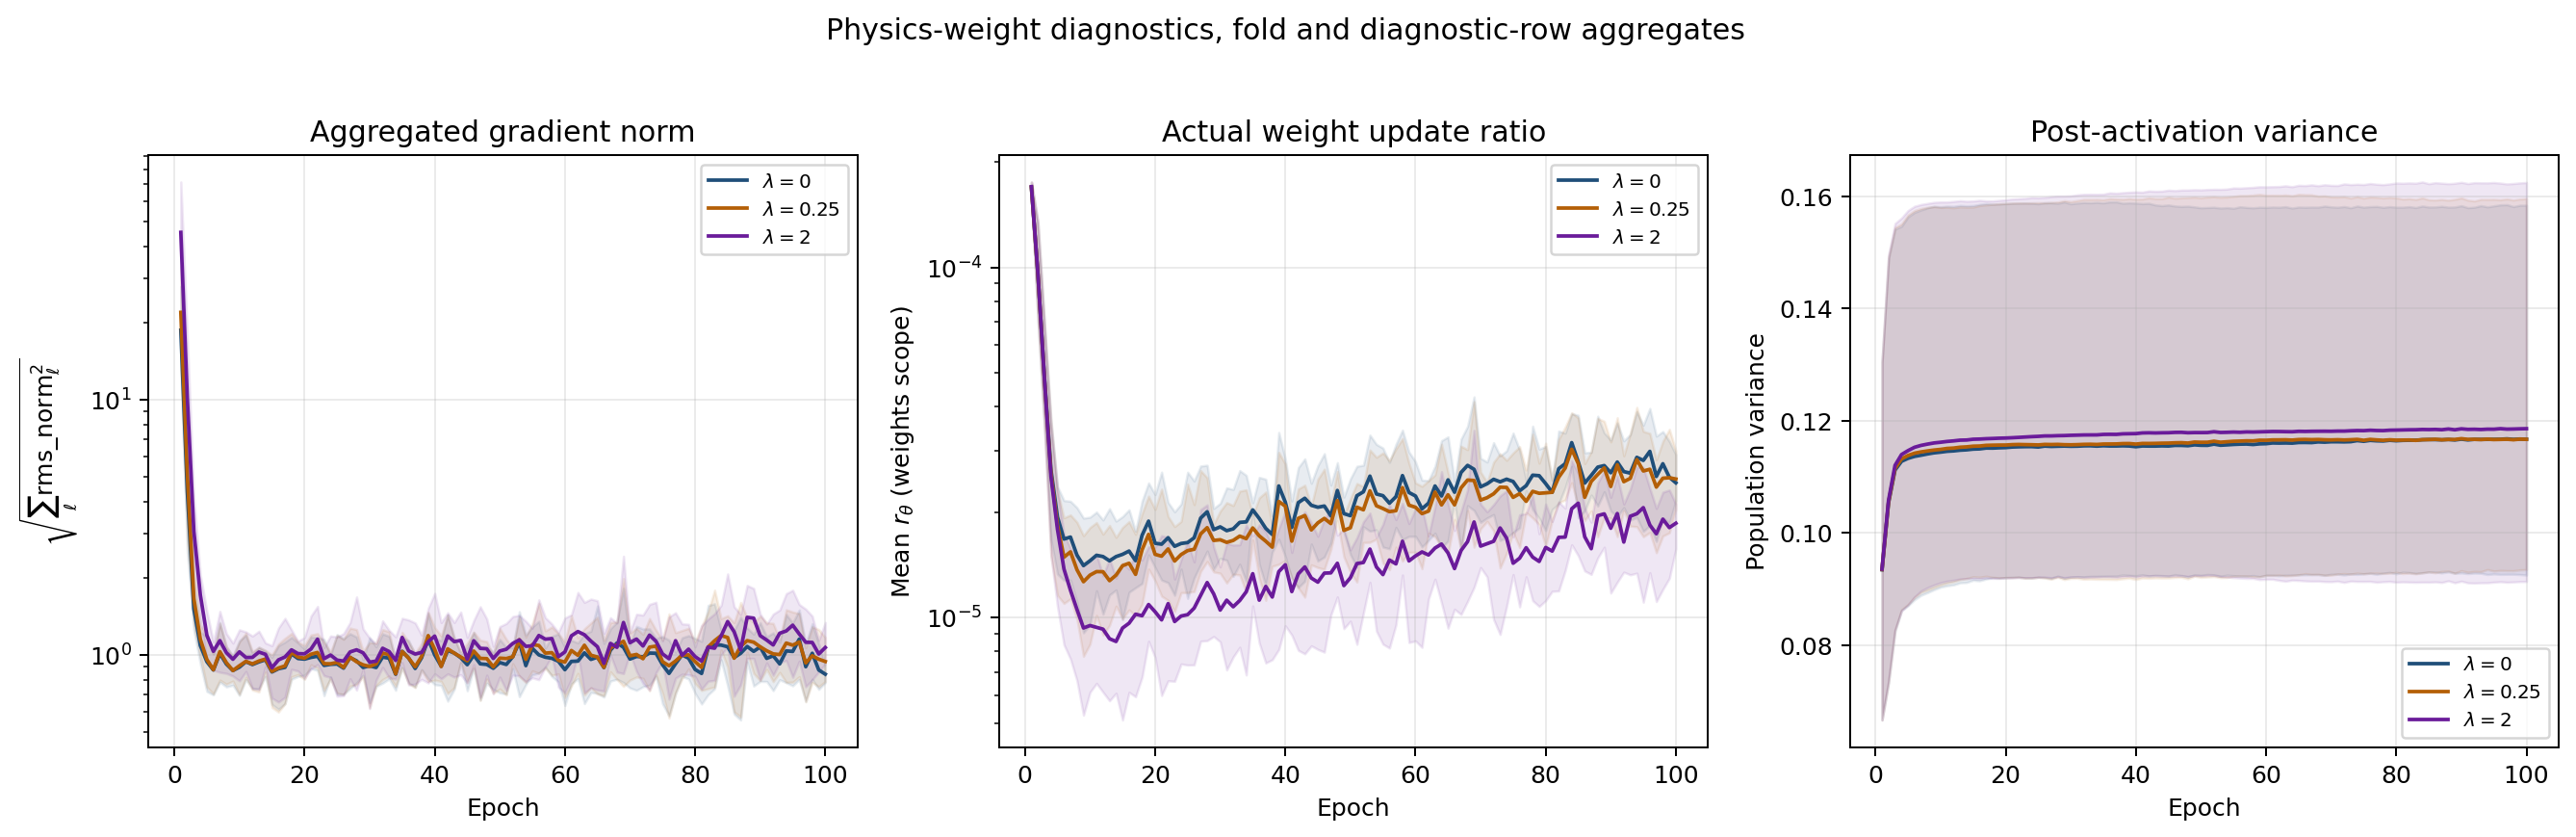
\includegraphics[width=0.98\linewidth]{Images/Chapter04/physics/physics_aggregate_diagnostics.png}
    \caption{Layer-agnostic diagnostics for the recorded physics-weight sweep. Curves are means over folds and comparable diagnostic rows, with minimum to maximum fold bands. The gradient panel uses the square root of the sum of squared per-layer RMS norms for the all-parameter scope, the update panel uses the actual weights-scope update ratio, and the variance panel uses post-activation population variance. No layer index is shown.}
    \label{fig:04_physics_diagnostics}
\end{figure}

The diagnostics also reveal that the physics term had a minimal effect on the network's internal dynamics:
\begin{itemize}
    \item[-] the middle panel shows that the "actual update ratio" for the model weights follows a very similar trajectory for all values of $\lambda$, decreasing steadily as the models converge. For the baseline model, this ratio decreased from an initial value of approximately $1.69\times 10^{-4}$ to $2.43\times 10^{-5}$ by the final epoch, indicating that the parameter updates became smaller and more refined over time;
    \item[-] the right panel demonstrates that the post-activation variance was almost completely unaffected by the physics term. For both $\lambda=0$ and $\lambda=2$, the variance remained around $0.1092$ after an initial transient. This is a crucial finding, as it rules out "vanishing" or "exploding" activations as a cause for the degraded performance.
\end{itemize}
\vspace{2ex}

The cross-validation experiment identifies the purely data-driven model with $\lambda=0$ as the unconstrained winner, achieving the lowest validation MSE of $0.005600634\pm0.001099091$. The diagnostic analysis confirms that the physics-informed loss term did not cause numerical instability or signal attenuation, but rather introduced a slight optimization compromise against the high-fidelity CFD ground truth.\\

Nevertheless, the final production model adopts a physics weight of $\lambda=0.10$. This decision is motivated by the project requirement of developing a Physics-Informed Neural Network surrogate model, which necessitates embedding theoretical domain knowledge ($\lambda > 0$). Under this operational constraint, $\lambda=0.10$ emerges as the optimal admissible choice: its validation error increase relative to the unconstrained baseline is merely $+0.000028$, a magnitude more than an order of magnitude smaller than the cross-validation fold standard deviation ($\approx 0.0011$), rendering its empirical impact statistically indistinguishable from zero. Furthermore, retaining this mild physical weight provides valuable structural grounding to classical Thin-Airfoil Theory ($C_L \approx 2\pi\alpha$) in the linear pre-stall regime ($|\alpha|\leq 10^\circ$), while completely avoiding the severe gradient inflation and loss landscape distortion observed at larger values such as $\lambda=2.0$. Consequently, $\lambda=0.10$ represents the most robust and sound compromise between physical consistency and empirical predictive accuracy.

\subsection{Weight regularization}
\label{sec:04_regularization_tuning}

Weight regularization was tested because the dense head contains millions of trainable weights, so reducing unnecessary parameter magnitude could in principle improve validation performance. As we can see in \cite{tibshirani1996lasso} and \cite{hoerl1970ridge}, L1 regularization is associated with sparsity and L2 regularization with continuous shrinkage. The central question was whether these penalties could provide a benefit, or if they would instead hinder optimization or introduce unnecessary bias, particularly if the unregularized model was not significantly overfitting.\\

For every convolutional and dense weight tensor $W_\ell$, the implementation defines the two penalties as:
\begin{equation}
    R_{\mathrm{L1}}=\lambda_1\sum_{\ell}\sum_{w\in W_\ell}|w|,
    \qquad
    R_{\mathrm{L2}}=\lambda_2\sum_{\ell}\sum_{w\in W_\ell}w^2.
    \label{eq:04_regularization}
\end{equation}
The regularization is applied to the weights only, without considering the biases. The coefficients $\lambda_1$ and $\lambda_2$ are passed via \texttt{LossConfig}, allowing \texttt{Trainer} to compute the regularization gradients directly on the weights after distributed MPI synchronization and prior to gradient clipping. The corresponding gradient term, $\lambda_1\,\operatorname{sign}(w)+2\lambda_2 w$, was added to the main loss gradient before the Adam update step. This implementation is distinct from the weight decay mechanism built into some optimizers.\\

To isolate the effects of regularization, we performed two independent, one-dimensional sweeps for the L1 and L2 coefficients ($\lambda_1$ and $\lambda_2$), starting from a baseline of zero for both:
\begin{itemize}
    \item[-] for L1, we evaluated eight values from $6.75\times 10^{-7}$ to $6.75\times 10^{-4}$, with zero as the reference;
    \item[-] for L2, we evaluated eight values from $10^{-4}$ to $10^{-1}$, with zero as the reference. 
\end{itemize}
All other hyperparameters were held constant. The full comparison followed the rigorous cross-validation framework detailed in Section \ref{sec:04_cross_validation}.\\

The results from both the L1 and L2 sweeps, presented in Tables \ref{tab:04_l1_results} and \ref{tab:04_l2_results}, point to the same clear conclusion: weight regularization did not improve model performance.

\begin{table}[h!]
    \centering
    \begin{tabular}{rccrr}
        \hline
        $\lambda_1$ & Mean validation MSE & Fold standard deviation & $\Delta_{\lambda_1}$ & Improved folds \\
        \hline
        0 & 0.004419 & 0.000794 & 0 & -- \\
        $6.75\times10^{-7}$ & 0.004424 & 0.000788 & +0.0000053 & 2/5 \\
        $2.13\times10^{-6}$ & 0.004436 & 0.000800 & +0.0000178 & 2/5 \\
        $6.75\times10^{-6}$ & 0.004478 & 0.000811 & +0.0000588 & 0/5 \\
        $2.13\times10^{-5}$ & 0.004540 & 0.000832 & +0.0001209 & 0/5 \\
        $6.75\times10^{-5}$ & 0.004684 & 0.000902 & +0.0002656 & 0/5 \\
        $2.13\times10^{-4}$ & 0.005100 & 0.000950 & +0.0006810 & 0/5 \\
        $6.75\times10^{-4}$ & 0.006462 & 0.001189 & +0.0020431 & 0/5 \\
        \hline
    \end{tabular}
    \caption{Documented L1 reference sweep on the large topology. Values are transcribed from the experiment README because the corresponding raw result tree is absent. $\Delta_{\lambda_1}$ is the documented candidate minus reference mean validation MSE.}
    \label{tab:04_l1_results}
\end{table}

\begin{table}[h!]
    \centering
    \begin{tabular}{rccrr}
        \hline
        $\lambda_2$ & Mean validation MSE & Fold standard deviation & $\Delta_{\lambda_2}$ & Improved folds \\
        \hline
        0 & 0.004419 & 0.000794 & 0 & -- \\
        $10^{-4}$ & 0.004483 & 0.000819 & +0.0000644 & 1/5 \\
        $3.16\times10^{-4}$ & 0.004580 & 0.000859 & +0.0001613 & 0/5 \\
        $10^{-3}$ & 0.004768 & 0.000932 & +0.0003489 & 0/5 \\
        $3.16\times10^{-3}$ & 0.005092 & 0.000992 & +0.0006730 & 0/5 \\
        $10^{-2}$ & 0.005902 & 0.001100 & +0.0014836 & 0/5 \\
        $3.16\times10^{-2}$ & 0.006994 & 0.001217 & +0.0025749 & 0/5 \\
        $10^{-1}$ & 0.008453 & 0.001080 & +0.0040345 & 0/5 \\
        \hline
    \end{tabular}
    \caption{Documented L2 reference sweep on the large topology. Values are transcribed from the experiment README because the corresponding raw result tree is absent. $\Delta_{\lambda_2}$ is the documented candidate minus reference mean validation MSE.}
    \label{tab:04_l2_results}
\end{table}

In both experiments, the baseline model with zero penalty ($\lambda=0$) achieved the lowest mean validation MSE of $0.004419 \pm 0.000794$; 
\begin{itemize}
    \item[-] the nearest L1 candidates were only $5.3\times10^{-6}$ and $1.78\times10^{-5}$ worse in the reported mean and improved in two folds, so neither meets the four-fold paired criterion or exceeds its own paired spread;
    \item[-] the nearest L2 candidate, $10^{-4}$, improved in one fold and was worse by $6.44\times10^{-5}$ in the reported mean. The degradation then increased across the tested grids.
\end{itemize}
At the same time, the validation minus training gap decreased, but the training MSE rose faster, indicating that shrinkage restricted the fit more than it corrected overfitting in this fixed 100-epoch regime.\\

The documented cross-validation winner is therefore $\lambda_1=0$ and $\lambda_2=0$, with reported mean physical validation MSE $0.004419\pm0.000794$. The current production source also sets both penalties to zero, so the direction of this choice agrees with \texttt{CNN/main.cpp}. 

\subsection{Activation-function tuning}
\label{sec:04_activation_tuning}

The activation function determines the nonlinear transformation applied after an affine layer and therefore affects both the signal passed to the next layer and the gradient returned during backpropagation. This choice is particularly relevant for the selected topology, which contains one activation after the convolution and four more in the dense head.\\

This experiment compares several common activation functions to determine which is most effective for our specific architecture and aerodynamic prediction task. The purpose was not to assume that one family is universally better, but to measure which transformation gives the lowest physical validation error under the fixed architecture and training budget. Saturating nonlinearities can reduce the derivative when their input has large magnitude, whereas a rectifier retains a unit derivative on its positive branch; these are established mechanisms for changes in signal and gradient propagation, as stated by \cite{glorot2010understanding}.\\

From the rectifier family, we tested the standard ReLU, which deactivates for negative inputs, and several variants of LeakyReLU, which allow a small non-zero gradient to pass through, preventing the "dying ReLU" problem:
\begin{equation}
\begin{aligned}
    f_{\mathrm{ReLU}}(x)&=\begin{cases}
        x, & x>0,\\
        0, & x\leq0,
    \end{cases}
    & f_{\mathrm{ReLU}}'(x)&=\begin{cases}
        1, & x>0,\\
        0, & x\leq0,
    \end{cases}\\[1ex]
    f_{\alpha}(x)&=\begin{cases}
        x, & x>0,\\
        \alpha x, & x\leq0,
    \end{cases}
    & f_{\alpha}'(x)&=\begin{cases}
        1, & x>0,\\
        \alpha, & x\leq0.
    \end{cases}
\end{aligned}
    \label{eq:04_rectifier_activations}
\end{equation}
The experiment tested three different negative slopes for LeakyReLU: $\alpha\in\{0.01,0.05,0.1\}$.\\

The smooth alternatives were implemented as:
\begin{equation}
\begin{aligned}
    f_{\mathrm{Tanh}}(x)&=\tanh(x),
    & f_{\mathrm{Tanh}}'(x)&=1-\tanh^2(x),\\
    f_{\mathrm{Sigmoid}}(x)&=\frac{1}{1+\exp(-x)},
    & f_{\mathrm{Sigmoid}}'(x)&=f_{\mathrm{Sigmoid}}(x)\left(1-f_{\mathrm{Sigmoid}}(x)\right).
\end{aligned}
    \label{eq:04_saturating_activations}
\end{equation}
Their outputs are bounded, and the derivatives become small in the corresponding saturation regions. The final dense layer remains linear, so these transformations are used only in the convolutional branch and in the four hidden dense layers.\\

In this case, all runs used the same best-performing topology (from Section \ref{sec:04_topology_tuning}), Adam optimizer with learning rate $10^{-5}$, batch size 64, and 100 epochs. It also used a physics weight of 0.1, as stated at the end of Section \ref{sec:04_physics_weight_tuning}. The entire experiment followed the rigorous cross-validation framework and evaluation metrics detailed in Section \ref{sec:04_cross_validation}.\\

The results of the activation function sweep, summarized in Table \ref{tab:04_activation_results}, reveal a clear performance divide between the two families of functions tested.\\

\begin{table}[h!]
    \centering
    \begin{tabular}{lcc}
        \hline
        Activation & Mean validation MSE & Fold standard deviation \\
        \hline
        LeakyReLU, $\alpha=0.05$ & 0.004427 & 0.000865 \\
        LeakyReLU, $\alpha=0.01$ & 0.004448 & 0.000876 \\
        ReLU & 0.004454 & 0.000876 \\
        LeakyReLU, $\alpha=0.1$ & 0.004545 & 0.000966 \\
        Tanh & 0.005466 & 0.001045 \\
        Sigmoid & 0.008971 & 0.001250 \\
        \hline
    \end{tabular}
    \caption{Complete activation-function comparison on the fixed large topology. Means and deviations are the sample-weighted physical validation MSE and weighted population standard deviation from \texttt{cv\_summary.csv}; the ranking was performed over all six candidates.}
    \label{tab:04_activation_results}
\end{table}

The ReLU family of activations (ReLU and Leaky ReLU) decisively outperformed the classic bounded functions. The best overall performance was achieved by LeakyReLU with $\alpha=0.05$, which recorded a mean physical validation MSE of $0.0044274\pm0.0008653$. However, the performance difference among the top three candidates was extremely small. As the error bars in Figure \ref{fig:04_activation_ranking} show, the differences between the top three candidates are within the range of their fold-to-fold variability, indicating that while LeakyReLU with $\alpha=0.05$ is the best performer, the other two rectifiers are statistically very close.\\

In contrast, the Tanh and Sigmoid functions performed significantly worse. Tanh's validation error was over $23\%$ higher than the winner's, while Sigmoid's error was more than double. This performance gap suggests that these functions suffered from the "vanishing gradient" problem, where the gradients become near-zero in the saturation regions, effectively stalling the learning process in the network's deep layers.\\

The separation from the bounded alternatives was larger. Tanh reached $0.005465620520\pm0.001045446677$, about $23.4\%$ above the selected mean, while Sigmoid reached $0.008971404356\pm0.001250088488$, about twice the selected mean. Figure~\ref{fig:04_activation_ranking} displays the official weighted means and deviations. All 30 candidate-fold records completed with finite metrics, and no candidate was removed from the ranking because of a failed or divergent run.\\

\begin{figure}[H]
    \centering
    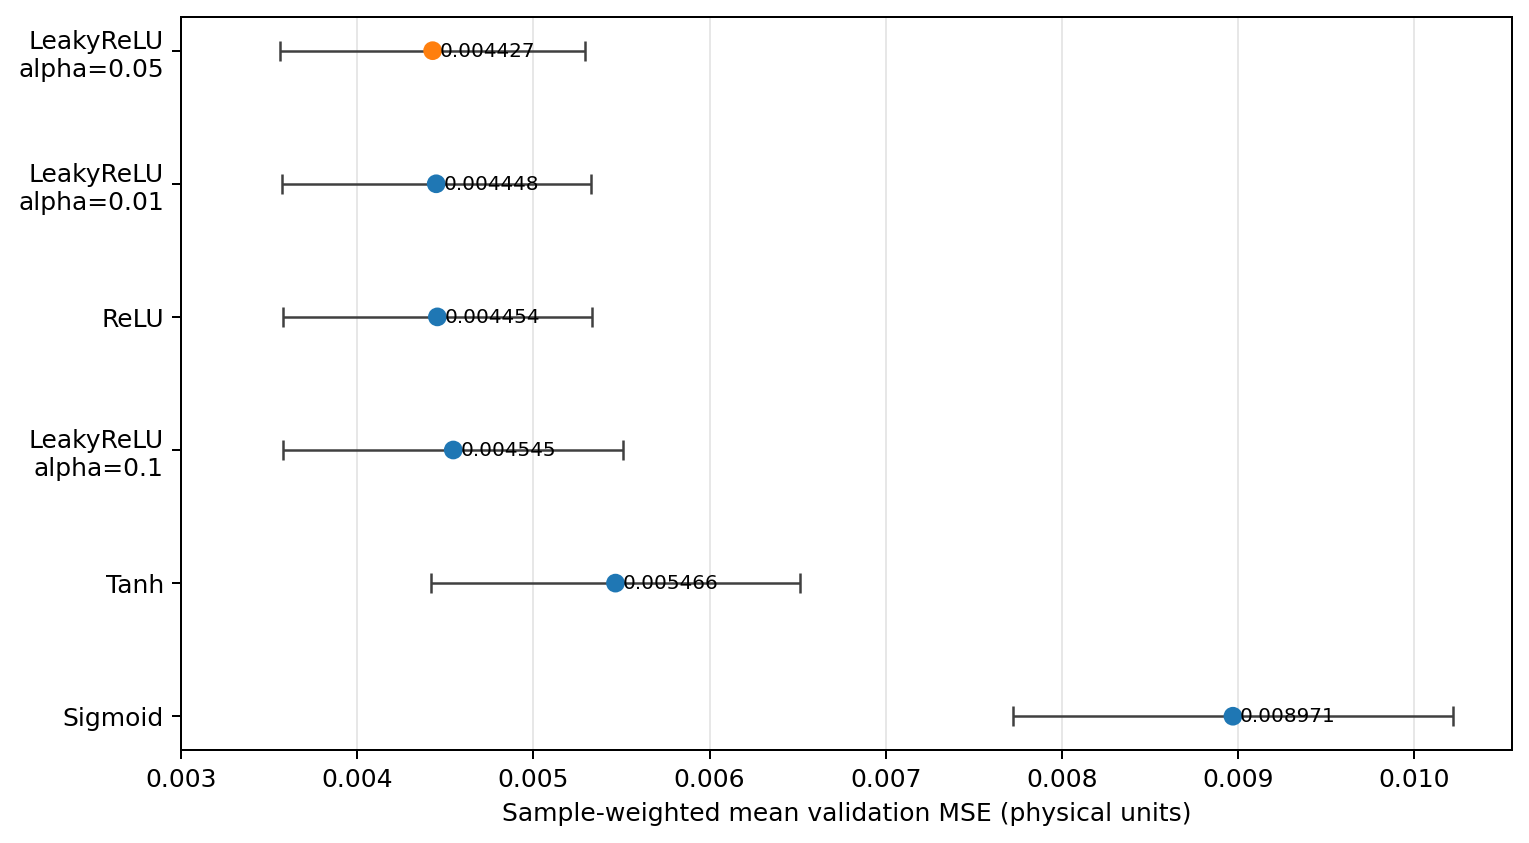
\includegraphics[width=0.80\linewidth]{Images/Chapter04/activation/activation_ranking.png}
    \caption{Complete activation-function ranking from the official \texttt{cv\_summary.csv}. Points are sample-weighted mean physical validation MSE values and horizontal error bars are the corresponding weighted population standard deviations over the five folds. The orange point identifies the lowest observed candidate, LeakyReLU with $\alpha=0.05$.}
    \label{fig:04_activation_ranking}
\end{figure}

The validation histories, presented in Figure \ref{fig:04_activation_history}, provide a view of the training process. The ReLU family candidates demonstrate fast and stable convergence, smoothly decreasing the validation error throughout the 100-epoch budget. In contrast, the saturing functions have a poorer convergence dynamics:
\begin{itemize}
    \item[-] Tanh converges to a solution that is consistently worse than any of the ReLU family functions;
    \item[-] Sigmoid performs by far the worst. It starts with a validation error more than an order of magnitude higher than the others. While it does improve over time, its convergence is extremely slow, and it never comes close to matching the performance of the non-saturating functions.
\end{itemize}
This convergence behavior strongly supports the hypothesis that the saturating functions are suffering from vanishing gradients.\\

\begin{figure}[H]
    \centering
    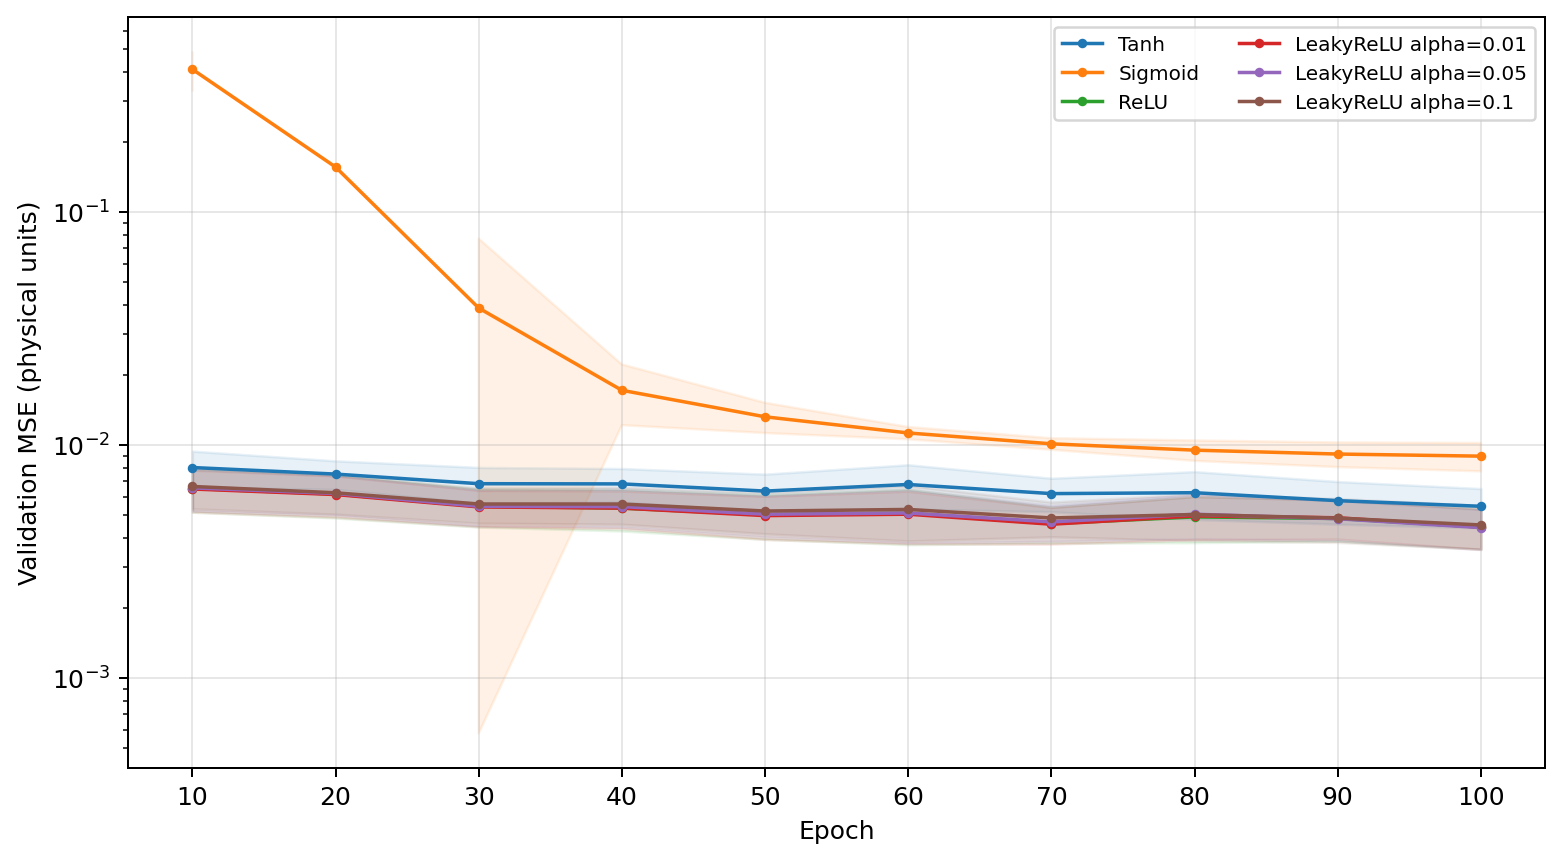
\includegraphics[width=0.75\linewidth]{Images/Chapter04/activation/activation_history.png}
    \caption{Fold-weighted physical validation MSE at the ten-epoch checkpoints for the six activation candidates. Shaded regions show the positive part of the weighted population standard deviation band over the five folds, and the vertical axis is logarithmic. The standardized SIMM training objective is not plotted on this axis.}
    \label{fig:04_activation_history}
\end{figure}

The recorded diagnostics provide a numerical stability check, but they do not change the selection rule. For gradient flow, we use rows with \texttt{parameter\_scope=all} and the stored \texttt{maximum\_norm} for peak checks. As we can see in the top panels of Figure \ref{fig:04_activation_diagnostics}, the largest value for the selected candidate was $20.1379$ at epoch 1, with similar peaks for ReLU and other LeakyReLU variants. Tanh was the numerical outlier with a peak of $111.508$: this early-epoch instability likely hindered its ability to find a good solution.\\

Sigmoid had a lower peak of $18.2200$, but this does not imply better optimization because its early validation curve was much worse. Indeed, the right panel confirms this instability, showing that Sigmoid resulted in the largest and most chaotic parametr updates, with a peak update ratio of $6.15050\times10^{-4}$. In contrast, the entire ReLU family, including the selected one, exhibited much smaller and more controlled updates, peaking aroung $4.5\times10^{-4}$.\\

In contrast, the bottom two panels show the detailed diagnostics for the winning LeakyReLU candidate. The gradients are well-behaved across the network’s depth. After an initial transient at epoch 1, the gradients at epoch 100 are small and stable, indicating smooth convergence without evidence of exploding gradients. The post-activation variance decreases toward the deepest hidden layers, but this reduction should not be interpreted by itself as signal degradation. Since the network ultimately performs scalar regression, the deeper layers progressively compress the high-dimensional representation into features that are directly useful for predicting $C_L$. Crucially, the variance remains clearly non-zero and stabilizes during training, providing no evidence of representational collapse.\\

\begin{figure}[H]
    \centering
    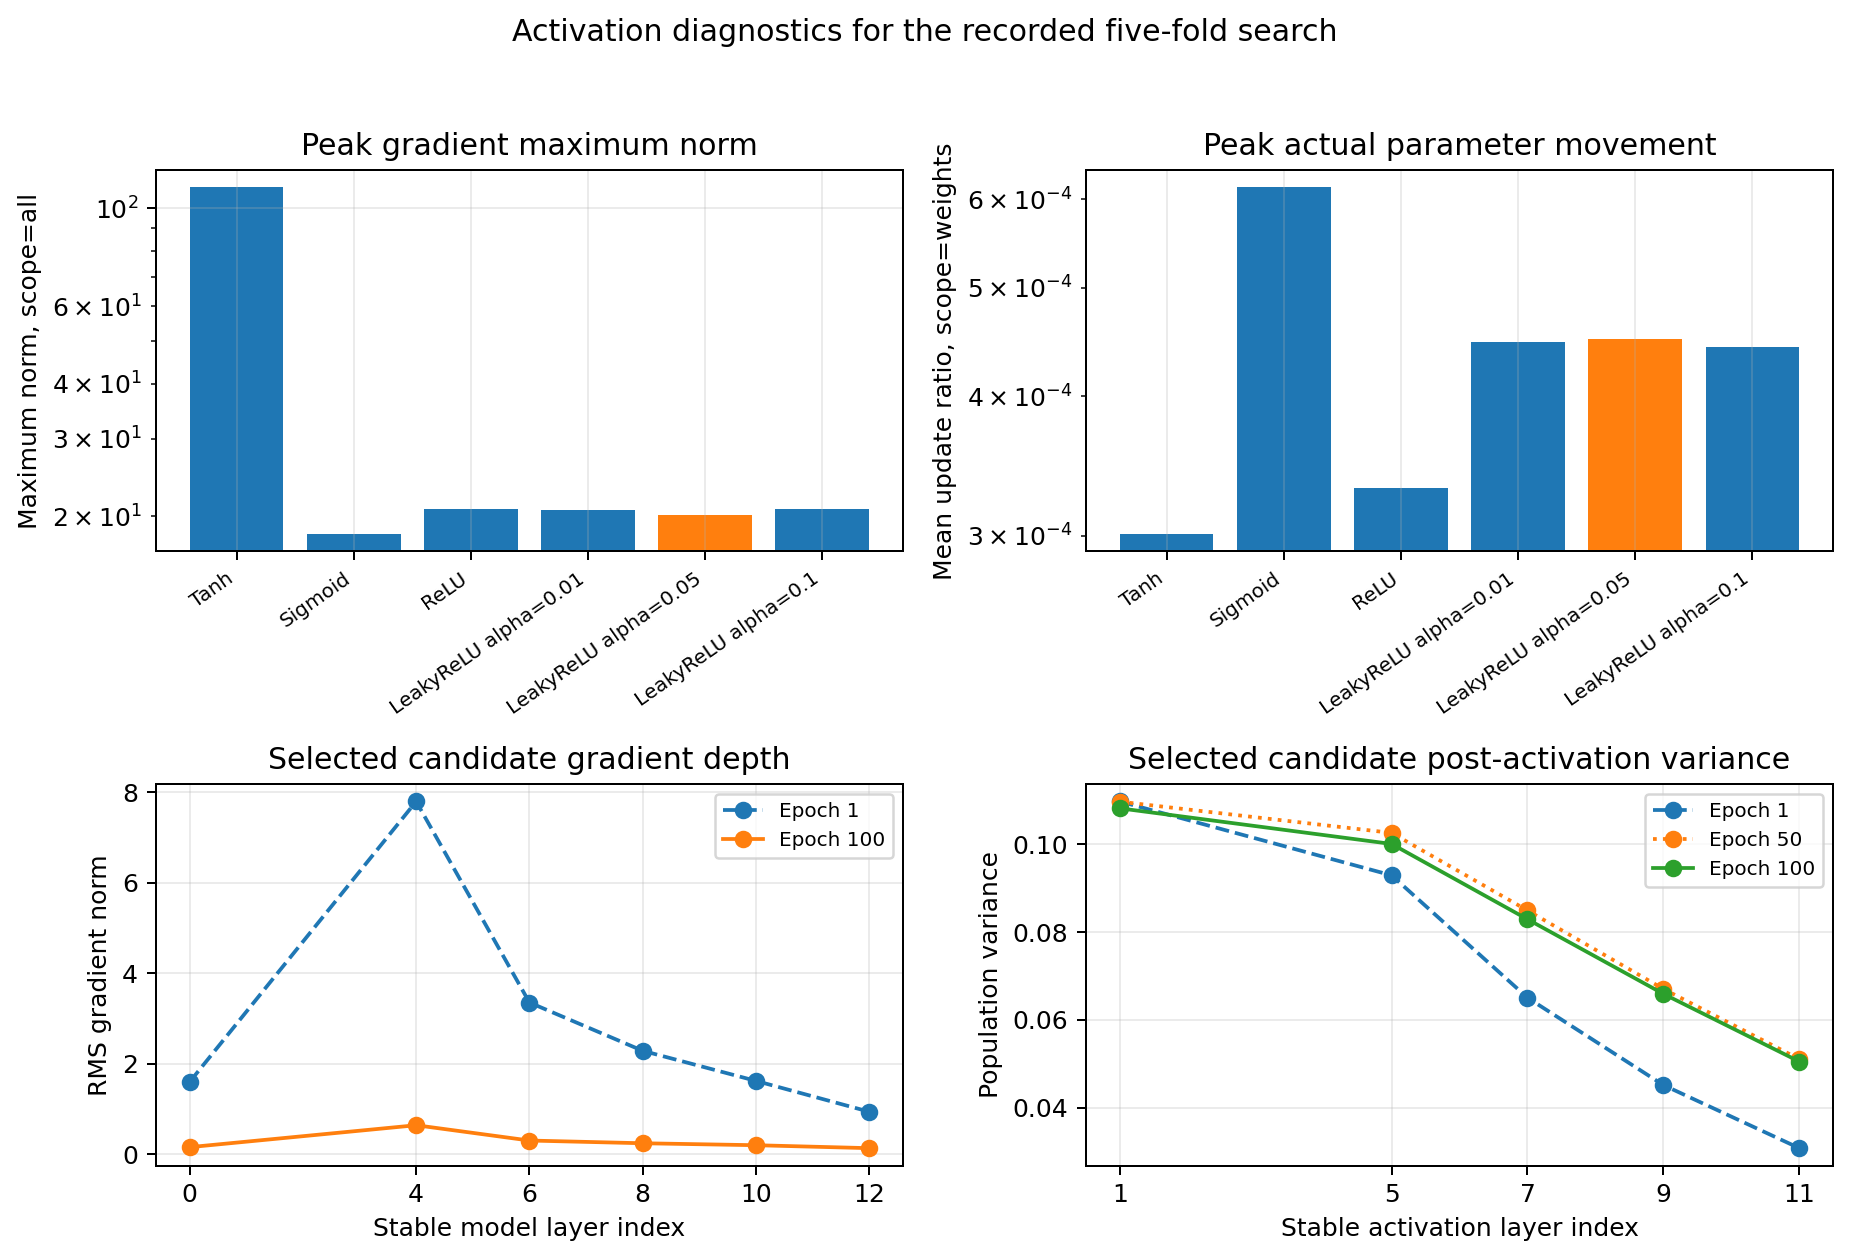
\includegraphics[width=0.95\linewidth]{Images/Chapter04/activation/activation_diagnostics.png}
    \caption{Diagnostics for the activation-function search. The upper panels show, for each candidate, the maximum gradient \texttt{maximum\_norm} with \texttt{parameter\_scope=all} and the maximum actual weight update ratio with \texttt{parameter\_scope=weights}, taken over all five folds, layers, and epochs. The lower left panel shows fold-averaged RMS gradient norms for the selected candidate at epochs 1 and 100 over stable trainable layer indices. The lower right panel shows post-activation population variances for the selected candidate at epochs 1, 50, and 100, pooled over folds from the recorded population moments.}
    \label{fig:04_activation_diagnostics}
\end{figure}

More in details, the activation statistics show the transformation expected from the equations. For the selected LeakyReLU, the post-activation population variances were pooled over folds from the recorded population moments as follows:
\begin{equation}
\begin{array}{c|ccccc}
\text{epoch} & \text{layer 1} & \text{layer 5} & \text{layer 7} & \text{layer 9} & \text{layer 11} \\
\hline
1   & 0.109805 & 0.092960 & 0.065048 & 0.045128 & 0.030745 \\
50  & 0.109755 & 0.102640 & 0.084950 & 0.067045 & 0.051060 \\
100 & 0.108244 & 0.100116 & 0.082939 & 0.065922 & 0.050486
\end{array}
\label{eq:04_activation_variance}
\end{equation}
The variance decreases through the dense head, but it does not collapse to zero and changes little between epochs 50 and 100. The full selected-candidate diagnostic range was approximately $[-4.003,4.035]$ before activation and $[-0.200,4.035]$ after activation, which is consistent with retaining a scaled negative branch. The corresponding ReLU post-activation minimum was exactly zero. These observations support controlled negative attenuation and a stable signal scale for the selected run, although they do not establish that this mechanism alone caused its small validation advantage.\\

Conversely, the diagnostics provide clear evidence that the bounded functions failed due to neuron saturation. For Tanh, post-activation values were recorded as high as $0.9994$, extremely close to the function's limit where the derivative is nearly zero. The issue was even more pronounced for Sigmoid, where pre-activation values late in training reached as high as $10.67$, deep into the saturation region. This behavior is perfectly consistent with the vanishing gradient hypothesis and directly explains the slow, ineffective convergence observed in the main results.\\

The vanishing-gradient risk is most directly assessed from the distribution of the pre-activation value $z$, rather than from the post-activation value alone. If $a_j=f_j(z_j)$, the chain rule inserts one derivative factor at every nonlinear layer. Ignoring the separate linear weight transformations, the activation contribution along a path through $k$ nonlinearities is:
\begin{equation}
    \frac{\partial\mathcal{L}}{\partial z_j}
    =\frac{\partial\mathcal{L}}{\partial a_j}f_j'(z_j)
    \qquad
    G_{\mathrm{act}}(k)=\prod_{j=1}^{k}\left|f_j'(z_j)\right|
    \label{eq:04_activation_chain_gradient}
\end{equation}
When the actual values $z_j$ fall in a plateau, $G_{\mathrm{act}}$ becomes small even when the upstream loss gradient is non-zero. A broad or heavy-tailed pre-activation distribution therefore raises the fraction of samples and paths that receive weak local gradients; it does not imply that every path vanishes, because values near the central high-slope region can still carry a useful signal.\\

The scale of this effect is substantial. For Sigmoid, the derivative at an input of 5 is already tiny ($|f'(5)|\simeq6.65\times10^{-3}$). To illustrate the multiplicative impact, if a gradient passed through just five such saturated neurons, it would be attenuated by a factor of approximately $10^{-11}$. For Tanh, the effect is even more extreme. Our diagnostic data confirms this was happening, with pre-activation values for Sigmoid reaching as high as 10.67 late in training, well into the saturation region. This mechanism provides a definitive explanation for the slow and ineffective convergence of these functions.\\

The rectifiers have a different but equally important failure mode. ReLU has an exact zero derivative for $z\leq0$, so a unit whose inputs remain on the negative branch contributes no local gradient through that activation. LeakyReLU replaces this strict plateau with a constant negative-branch slope $\alpha$. This avoids an exactly dead path, but it does not eliminate attenuation: $k$ consecutive negative-branch traversals contribute $\alpha^k$, so the tested $\alpha=0.05$ can still multiply the signal by $0.05^k$, while $\alpha=0.01$ attenuates it more strongly and $\alpha=0.1$ less strongly. Thus, "non-saturating" should not be interpreted as "immune to vanishing gradients"; the relevant question is how much of the observed pre-activation distribution lies in each branch and how those branches are arranged across depth.\\

\begin{figure}[H]
    \centering
    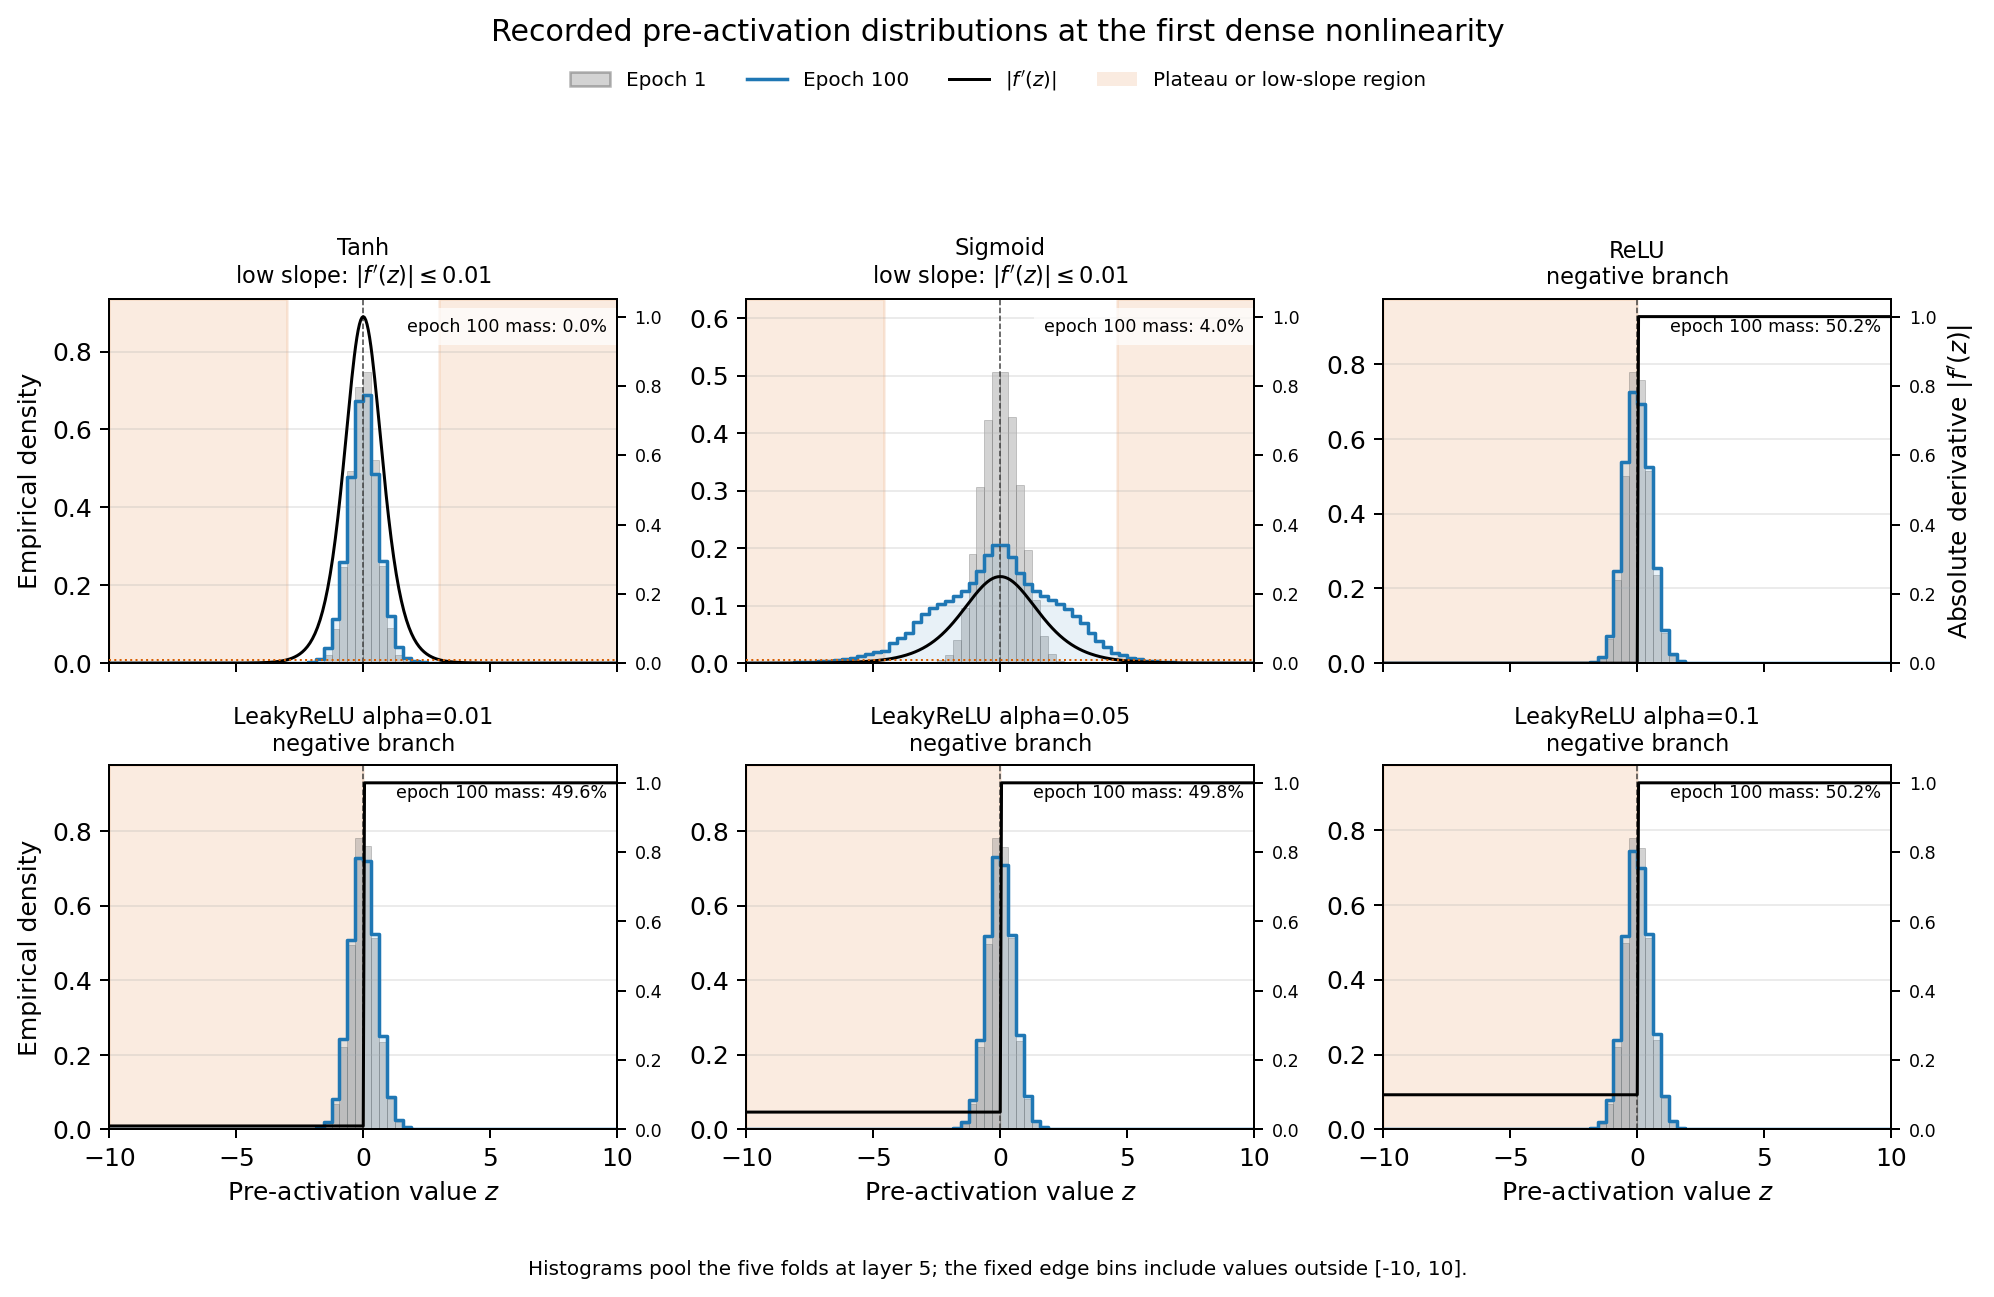
\includegraphics[width=0.98\linewidth]{Images/Chapter04/activation/activation_input_distributions.png}
    \caption{Empirical distributions of the actual pre-activation values $z$ at the first dense nonlinearity (stable model layer 5) for the six activation candidates. Gray bars show epoch 1 and blue step curves show epoch 100, with histograms pooled over the five folds. The black curves show the exact absolute derivative $|f'(z)|$ on the right-hand scale. Orange shading identifies the Tanh and Sigmoid regions with $|f'(z)|\leq0.01$ and the negative branch for ReLU and LeakyReLU. The epoch-100 mass annotations are approximate because the committed diagnostics store fixed-bin counts; the edge bins include values outside the displayed $[-10,10]$ range.}
    \label{fig:04_activation_input_distributions}
\end{figure}

This theoretical risk of vanishing gradients is confirmed by the empirical data. Figure \ref{fig:04_activation_input_distributions} visualizes the distribution of the actual pre-activation values ($z$) at the first dense layer, providing a clear picture of why the different activation functions performed so differently.\\

The plot for Sigmoid is the most revealing. By epoch 100, the distribution of its pre-activation values has broadened significantly. Approximately $4.0\%$ of its inputs now fall into the low-derivative "saturation" region (shaded in orange), where the gradient is less than $1\%$ of its maximum. This provides direct, visual proof that a substantial portion of the neurons are receiving near-zero gradients, which explains the function's extremely slow convergence. While Tanh does not show a significant mass in the saturation region in this specific layer, other diagnostics confirmed that saturation was occurring elsewhere in the network.\\

In contrast, the plots for the ReLU family show that roughly half of their inputs fall into the negative branch (also shaded). For standard ReLU, this means that $50.2\%$ of its neurons are "off" and passing a zero gradient. For the winning Leaky ReLU ($\alpha=0.05$), approximately $49.8\%$ of its inputs are in the negative branch, but they are passing a small, non-zero gradient. This visualization illustrates the key trade-off. While nearly half the neurons are in a low-gradient state for the ReLU family, this state is not catastrophic. The non-saturating positive branch allows strong gradients to flow, and the "leaky" negative branch prevents the complete death of neurons. This is a far healthier dynamic than the severe, widespread gradient attenuation caused by saturation in the bounded functions.\\

The final refit of the selected activation used all 1713 training samples and retained the large search topology. Its training SIMM objective decreased from $0.286768$ at epoch 1 to $0.00865917$ at epoch 100. The final MSE on the 429-sample test set was $0.00273892$. This is a post-selection estimate for the refitted activation-search model and must not be presented as the test performance of the ordinary production model.\\

The cross-validation winner is therefore \texttt{LeakyReLU} with $\alpha=0.05$, with physical validation MSE $0.00442742\pm0.00086526$ on the fixed large topology.

\subsection{Learning-rate and schedule tuning}
\label{sec:04_learning_rate_tuning}

After choosing the topology, optimizer, loss settings and activation, we studied the learning rate because it controls the scale and duration of the parameter updates. In Adam, the learning rate multiplies the bias-corrected adaptive direction; it is therefore not removed by the coordinate-wise denominator, even though that denominator adapts to the history of each parameter. A rate that is too small may lead to slow convergence, falling to reach an optimal solution within the fixed epoch budget. Conversely, a rate that is too large can cause the optimization to become unstable and diverge.\\

Beyond the learning rate's magnitude, its schedule, that represents how it changes over time, is also crucial. In addition to a constant rate, we tested step decay, cosine decay\footnote{That has been studied as part of the SGDR family \citep{loshchilov2017sgdr}} and warm-up, that was introduced to address early optimization difficulties in large-minibatch stochastic-gradient training \citep{goyal2017accurate}. Those references motivate the schedule families tested here, but they do not predict the behaviour of this Adam run: the present experiment uses no warm restarts, a different optimizer and a different data set.\\

The goal was to identify the combination of learning rate and schedule that leads to the fastest and most stable convergence for our specific aerodynamic modeling task.\\

Let $e\in\{0,\ldots,E-1\}$ denote the zero-based epoch index and let $E$ be the total number of epochs. The experiment evaluated four distinct types of learning rate schedules:
\begin{itemize}
    \item[-] in the constant rate, the learning rate remains fixed at its initial value $\eta_0$ throughout the training process:
    \begin{equation*}
    \eta_e=\eta_0
    \end{equation*}
    \item[-] in the step decay, the learning rate is multiplied by a decay factor $\gamma$ at fixed step intervals $S$:
    \begin{equation*}
    \eta_e=\eta_0\gamma^{\lfloor e/S\rfloor}
    \end{equation*}
    The step schedules change at zero-based indices $e=30,60,90$ for $S=30$, and at $e=15,30,45,60,75,90$ for $S=15$, which correspond to completed epochs 31, 61, 91 and 16, 31, 46, 61, 76, 91, respectively.
    \item[-] in the cosine decay, the learning rate smoothly anneals from a maximum value $\eta_{\max}$ to a minimum value $\eta_{\min}$ following a cosine curve:
    \begin{equation*}
    \eta_e=\eta_{\min}+\frac{1}{2}(\eta_{\max}-\eta_{\min})
    \left[1+\cos\left(\frac{e}{E-1}\pi\right)\right]
    \end{equation*}
    which reaches $\eta_{\max}$ at $e=0$ and $\eta_{\min}$ at $e=E-1$;
    \item[-] in the warm-up schedule, the training begins with a short linear "warm-up" phase, where the learning rate ramps up to a peak value, before following a cosine decay for the remainder of the training:
    \begin{equation*}
    \eta_e=\begin{cases}
        \eta_{\mathrm{start}}+\dfrac{e}{W}
        (\eta_{\mathrm{peak}}-\eta_{\mathrm{start}}), & 0\leq e<W,\\[6pt]
        \eta_{\min}+\dfrac{1}{2}(\eta_{\mathrm{peak}}-\eta_{\min})
        \left[1+\cos\left(\dfrac{e-W}{E-W-1}\pi\right)\right], & W\leq e<E,
    \end{cases}
    \end{equation*}
    where $W$ is the number of warm-up epochs. In the recorded grid, $E=100$, $W=5$, $\eta_{\mathrm{start}}=\eta_{\min}=10^{-5}$, and $\eta_{\mathrm{peak}}=10^{-1}$. Thus, the warm-up branch returns $10^{-5}$ at the first completed epoch and reaches $10^{-1}$ at completed epoch 6.
\end{itemize}
\vspace{2ex}

In the software architecture, each of these mathematical policies is implemented as a specialized subclass of the abstract \texttt{LRScheduler} base class (\texttt{ConstantLR}, \texttt{StepLR}, \texttt{CosineAnnealingLR} and \texttt{WarmupCosineLR}) and instantiated through an \texttt{LRSchedulerRecipe}. At the beginning of each epoch, the \texttt{Trainer} queries the active scheduler to adjust the optimizer's learning rate $\eta_e$ in a deterministic manner, ensuring full reproducibility across parallel MPI workers.\\

The grid search evaluated eleven candidates, which are summarized in Table \ref{tab:04_learning_rate_results}, combining the schedule types above with three different initial learning rate magnitudes: a low rate ($10^{-5}$), a medium rate ($10^{-3}$) and a high rate ($10^{-1}$). All experiments were performed using the winning activation function, LeakyReLU with $\alpha=0.05$, and the same fixed topology \texttt{conv5x5-dense-1024-512-256-128}. The other hyperparameters were kept constant, including the physics weight $0.1$, L1 and L2 weights $0$, dropout rate $0$, global batch size $64$, gradient clipping at $1$, and no early stopping. Each candidate was evaluated using the same five-fold cross-validation procedure as in the activation search, with 100 epochs per fold.

\begin{table}[h!]
    \centering
    \small
    \setlength{\tabcolsep}{3pt}
    \begin{tabularx}{\linewidth}{@{}
        >{\raggedright\arraybackslash}X
        >{\raggedright\arraybackslash}X
        >{\centering\arraybackslash}X
        >{\centering\arraybackslash}X
        @{}}
        \hline
        Candidate & Configuration & Mean validation MSE $\pm$ SD & Fold range \\
        \hline
        \texttt{const\_1e-3} & Constant, $\eta_0=10^{-3}$ & $0.003609\pm0.001335$ & $0.002092$ to $0.006094$ \\
        \texttt{step\_s15\_1e-3} & Step, $S=15$, $\gamma=0.5$, $\eta_0=10^{-3}$ & $0.004005\pm0.000704$ & $0.002826$ to $0.004779$ \\
        \texttt{step\_s30\_1e-3} & Step, $S=30$, $\gamma=0.1$, $\eta_0=10^{-3}$ & $0.004072\pm0.000785$ & $0.002865$ to $0.004955$ \\
        \texttt{const\_1e-5} & Constant, $\eta_0=10^{-5}$ & $0.004419\pm0.000790$ & $0.002880$ to $0.005001$ \\
        \texttt{step\_s30\_1e-5} & Step, $S=30$, $\gamma=0.1$, $\eta_0=10^{-5}$ & $0.005034\pm0.000901$ & $0.003434$ to $0.005786$ \\
        \texttt{step\_s15\_1e-5} & Step, $S=15$, $\gamma=0.5$, $\eta_0=10^{-5}$ & $0.005094\pm0.000905$ & $0.003484$ to $0.005861$ \\
        \texttt{cosine\_1e-1} & Cosine, $\eta_{\max}=10^{-1}$, $\eta_{\min}=10^{-5}$ & $5.577\e{8}\pm2.251\e{8}$ & $2.087\e{8}$ to $7.949\e{8}$ \\
        \texttt{warmup\_cosine\_1e-1} & Warm-up and cosine, $\eta_{\mathrm{peak}}=10^{-1}$ & $9.047\e{8}\pm8.866\e{8}$ & $1.207\e{8}$ to $2.507\e{9}$ \\
        \texttt{step\_s15\_1e-1} & Step, $S=15$, $\gamma=0.5$, $\eta_0=10^{-1}$ & $5.010\e{9}\pm2.956\e{9}$ & $1.530\e{9}$ to $9.316\e{9}$ \\
        \texttt{step\_s30\_1e-1} & Step, $S=30$, $\gamma=0.1$, $\eta_0=10^{-1}$ & $9.449\e{9}\pm4.726\e{9}$ & $3.197\e{9}$ to $1.631\e{10}$ \\
        \texttt{const\_1e-1} & Constant, $\eta_0=10^{-1}$ & $2.131\e{17}\pm3.116\e{17}$ & $1.843\e{16}$ to $8.313\e{17}$ \\
        \hline
    \end{tabularx}
    \caption{Complete ranking of the eleven learning-rate candidates. Means and deviations are the sample-weighted physical validation MSE and its weighted population standard deviation over the five folds, as recorded in \texttt{cv\_summary.csv}; the final column gives the minimum and maximum fold scores.}
    \label{tab:04_learning_rate_results}
\end{table}
\vspace{2ex}

The results of the learning rate sweep, shown also in Figure \ref{fig:04_learning_rate_ranking}, reveal a clear separation between the low-rate candidates and the high-rate candidates that reach $10^{-1}$.\\

The best performance was achieved by the constant learning rate of $10^{-3}$, which secured a mean validation MSE of $0.003609\pm0.001335$. This medium learning rate was consistently effective, winning four of the five cross-validation folds and delivering an $18\%$ error reduction compared to the constant $10^{-5}$ baseline. The nearest alternative is \texttt{step\_s15\_1e-3}, whose mean is $0.004005474214$; its lower dispersion does not compensate for the higher aggregate validation error under the stated selection rule.\\

\begin{figure}[H]
    \centering
    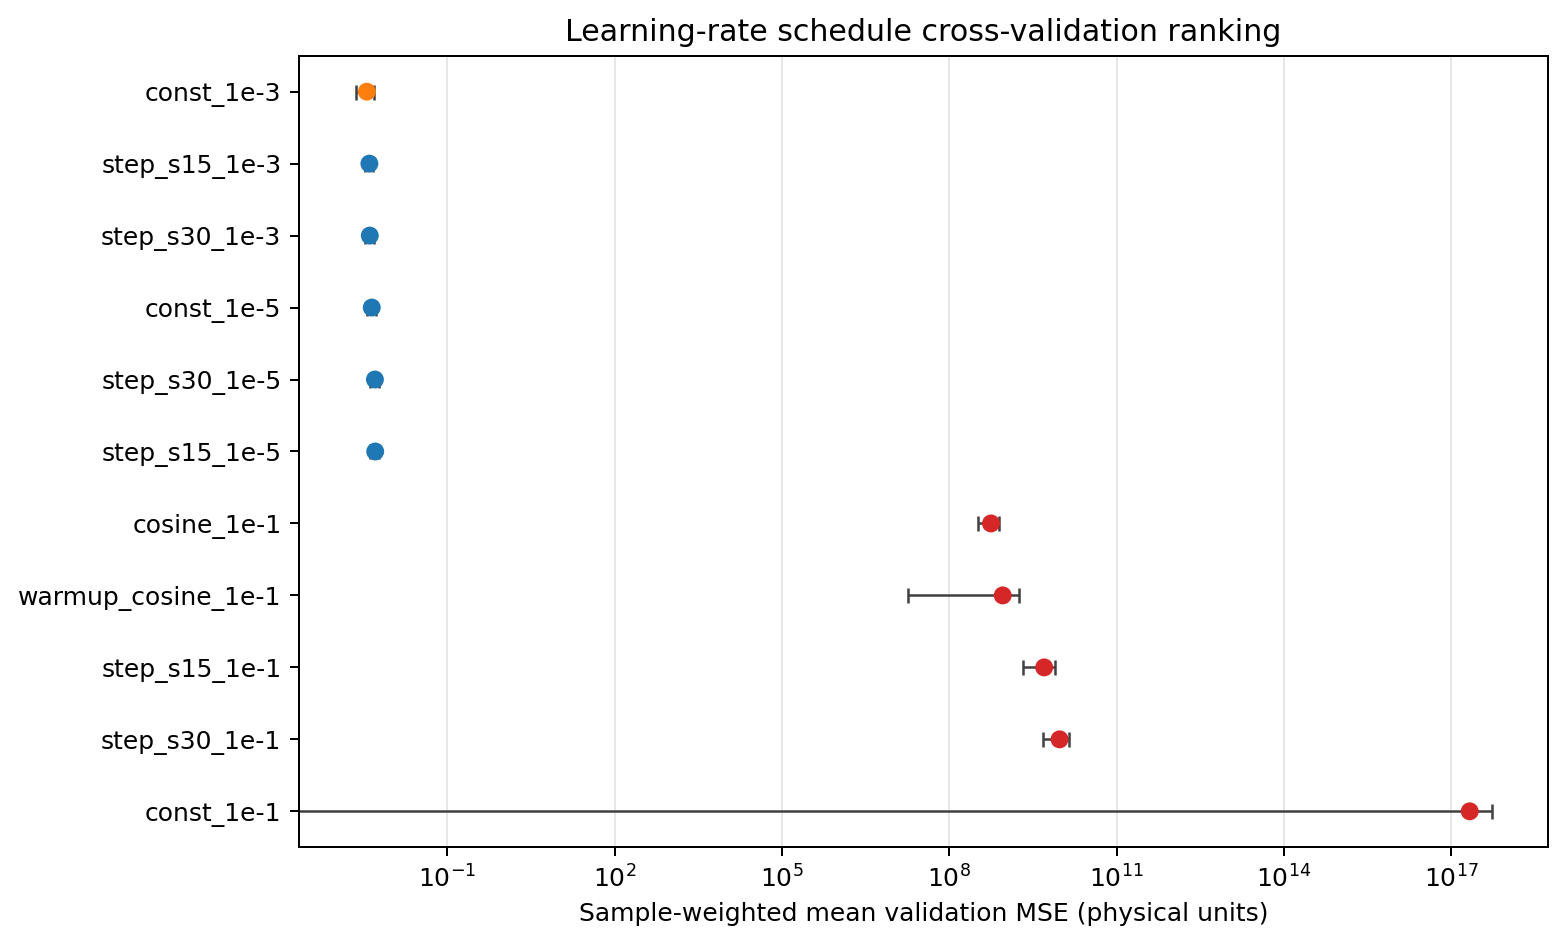
\includegraphics[width=0.90\linewidth]{Images/Chapter04/learning_rate/learning_rate_ranking.png}
    \caption{Complete learning-rate schedule ranking. Points show the sample-weighted mean physical validation MSE and horizontal bars show the weighted population standard deviation over five folds. The horizontal axis is logarithmic; orange identifies the selected constant $10^{-3}$ candidate and red identifies candidates whose rates reach $10^{-1}$.}
    \label{fig:04_learning_rate_ranking}
\end{figure}

In contrast, all candidates that used a high learning rate of $10^{-1}$ failed catastrophically. As shown by the red markers in Figure \ref{fig:04_learning_rate_ranking}, their validation errors were orders of magnitude higher, ranging from $10^{8}$ to $10^{17}$. This indicates that the optimization process diverged, likely due to an excessive step size in the parameter updates. Even the warm-up schedule, which initially starts at a safe low rate and ramps up to $10^{-1}$, suffered the same fate, demonstrating that even a brief exposure to this aggressive rate permanently destabilized training.\\

The convergence histories in Figure \ref{fig:04_learning_rate_history} provide a dynamic view of the training process and visually confirm the final rankings. The plot is split into two panels, distinguishing the behaviour of the stable and unstable learning rates:
\begin{itemize}
    \item[-] the top panel shows that all candidates with learning rates of $10^{-5}$ and $10^{-3}$ converge smoothly, with the constant $10^{-3}$ candidate achieving the lowest validation error. The $10^{-5}$ candidates, by contrast, converged much more slowly, indicating that their step sizes were too small to make optimal progress within the 100-epoch budget;
    \item[-] the bottom panel shows that the validation error for all the candidates that reach $10^{-1}$ immediately explodes to extreme values and remains many orders of magnitude above the stable group for the entire duration of training. Even for schedules that eventually decay the learning rate (like cosine and step decay), the initial instability was so severe that the models could never recover.
\end{itemize}
\vspace{2ex}
This analysis reinforces the conclusion that a learning rate of $10^{-3}$ represents a well-chosen spot, offering a balance between rapid convergence and numerical stability.\\

\begin{figure}[H]
    \centering
    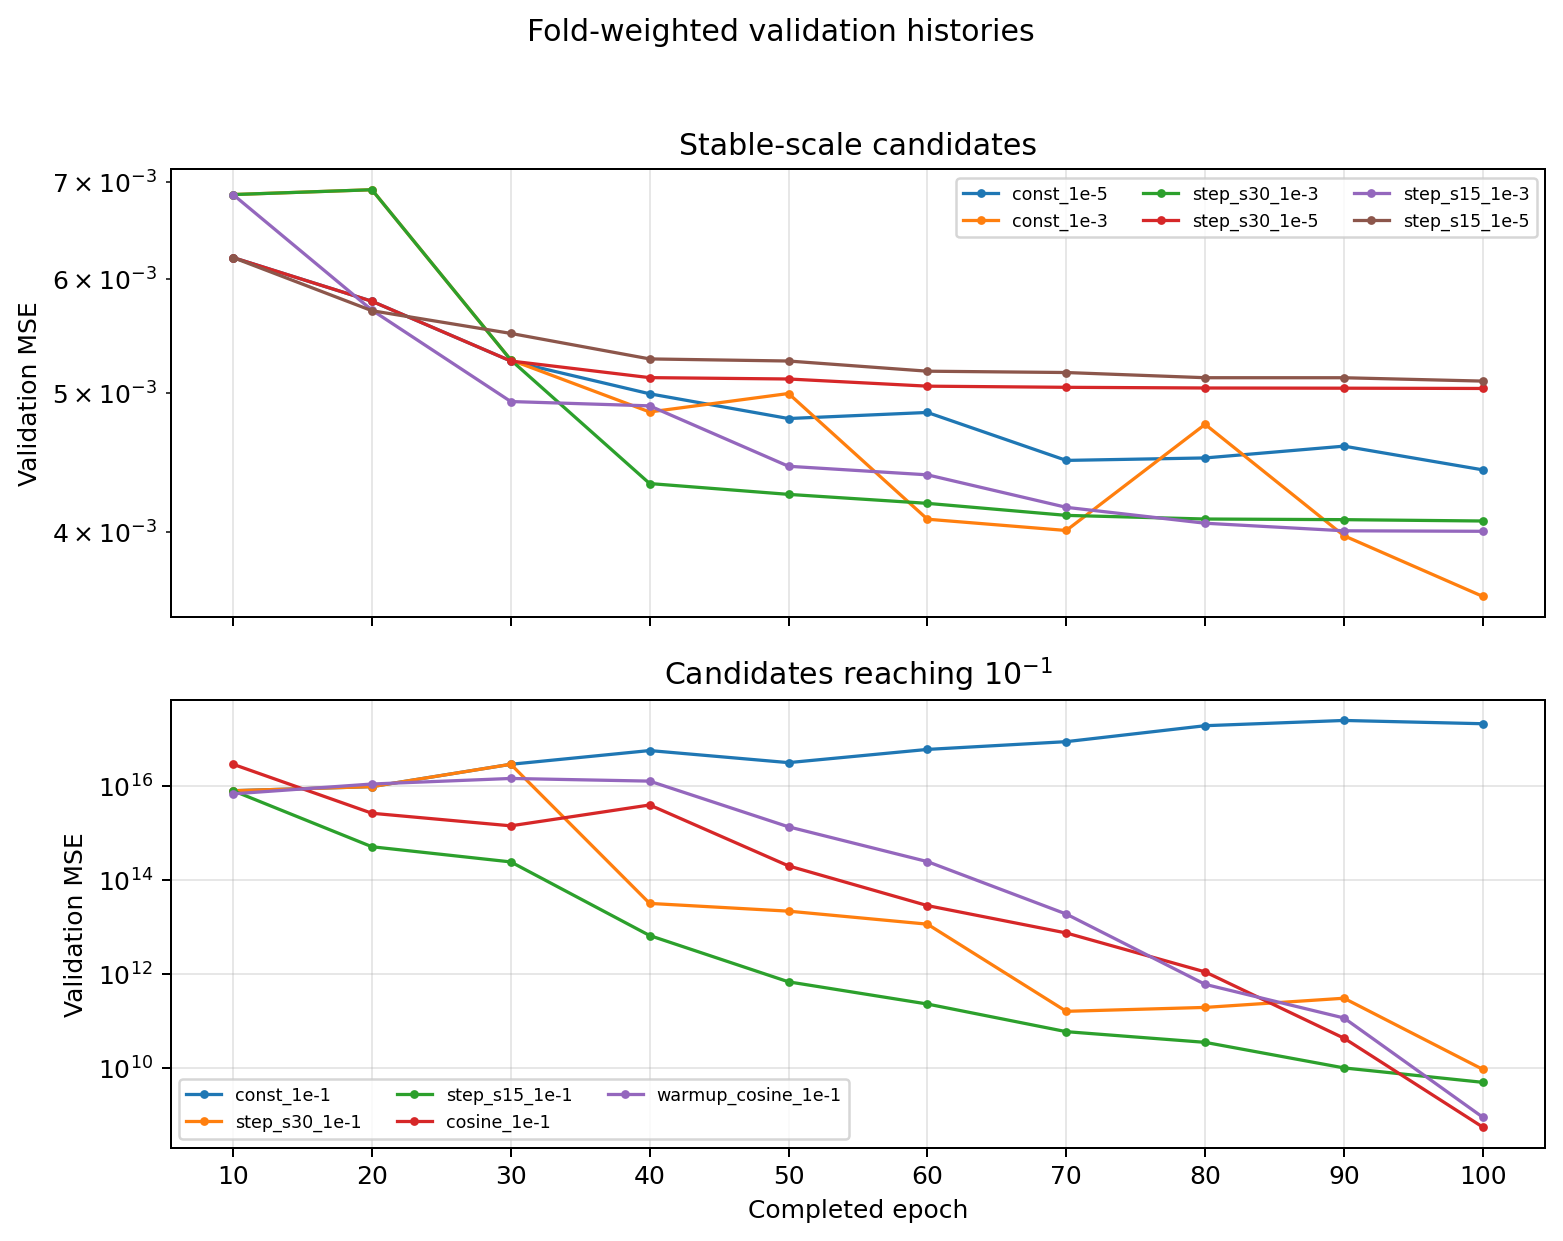
\includegraphics[width=0.90\linewidth]{Images/Chapter04/learning_rate/learning_rate_history.png}
    \caption{Sample-weighted validation histories at the ten-epoch checkpoints recorded for cross-validation. The upper panel contains the six candidates whose rates remain in the low-error scale, while the lower panel contains the five candidates that reach $10^{-1}$. Both vertical axes are logarithmic and show physical-unit MSE.}
    \label{fig:04_learning_rate_history}
\end{figure}

The divergence at $\eta = 10^{-1}$ stems from a fundamental mismatch between Adam's update dynamics and the network's weight scale:
\begin{itemize}
    \item[-] under Kaiming initialization, weights in the wide first dense layer ($D_{\mathrm{in}}=7202$) have a standard deviation of $\sigma = \sqrt{2/7202}\approx 0.0166$. Since Adam's coordinate update $\Delta \theta_j = -\eta \frac{\hat{m}_j}{\sqrt{\hat{v}_j}+\varepsilon}$ produces a step of magnitude $\approx \eta$ along active directions, setting $\eta = 0.1$ forces each parameter update to be approximately six times larger than the entire initial parameter scale in a single step. This immediately destroys the initial structural features, causing pre-activations and downstream predictions to blow up exponentially;
    \item[-] although component-wise gradient clipping ($\tilde{g}_{t,j}=\operatorname{clip}(g_{t,j},-1,1)$) prevents gradient norms from reaching infinity, Adam is scale-invariant. When gradients consistently saturate at the clipping threshold $\pm 1$, the ratio $\hat{m}/\sqrt{\hat{v}}$ remains $\approx \pm 1$, leaving the effective update size directly determined by $\eta=0.1$;
    \item[-] in schedules such as \texttt{warmup\_cosine\_1e-1}, the network trains stably during the first few epochs at low rates. However, as soon as $\eta$ hits $0.1$ at epoch 6, the parameters enter a high-loss, chaotic plateau. The moving moments $m_t$ and $v_t$ become corrupted by massive gradient noise, making it impossible for the optimizer to recover even when the cosine decay cools $\eta$ back down to $10^{-5}$ in later epochs.
\end{itemize}
\vspace{2ex}
Figure \ref{fig:04_learning_rate_schedules} tracks the effective learning rate profiles across completed epochs, highlighting how the transient peak at epoch 6 in the warm-up branch permanently derails optimization.\\

\begin{figure}[H]
    \centering
    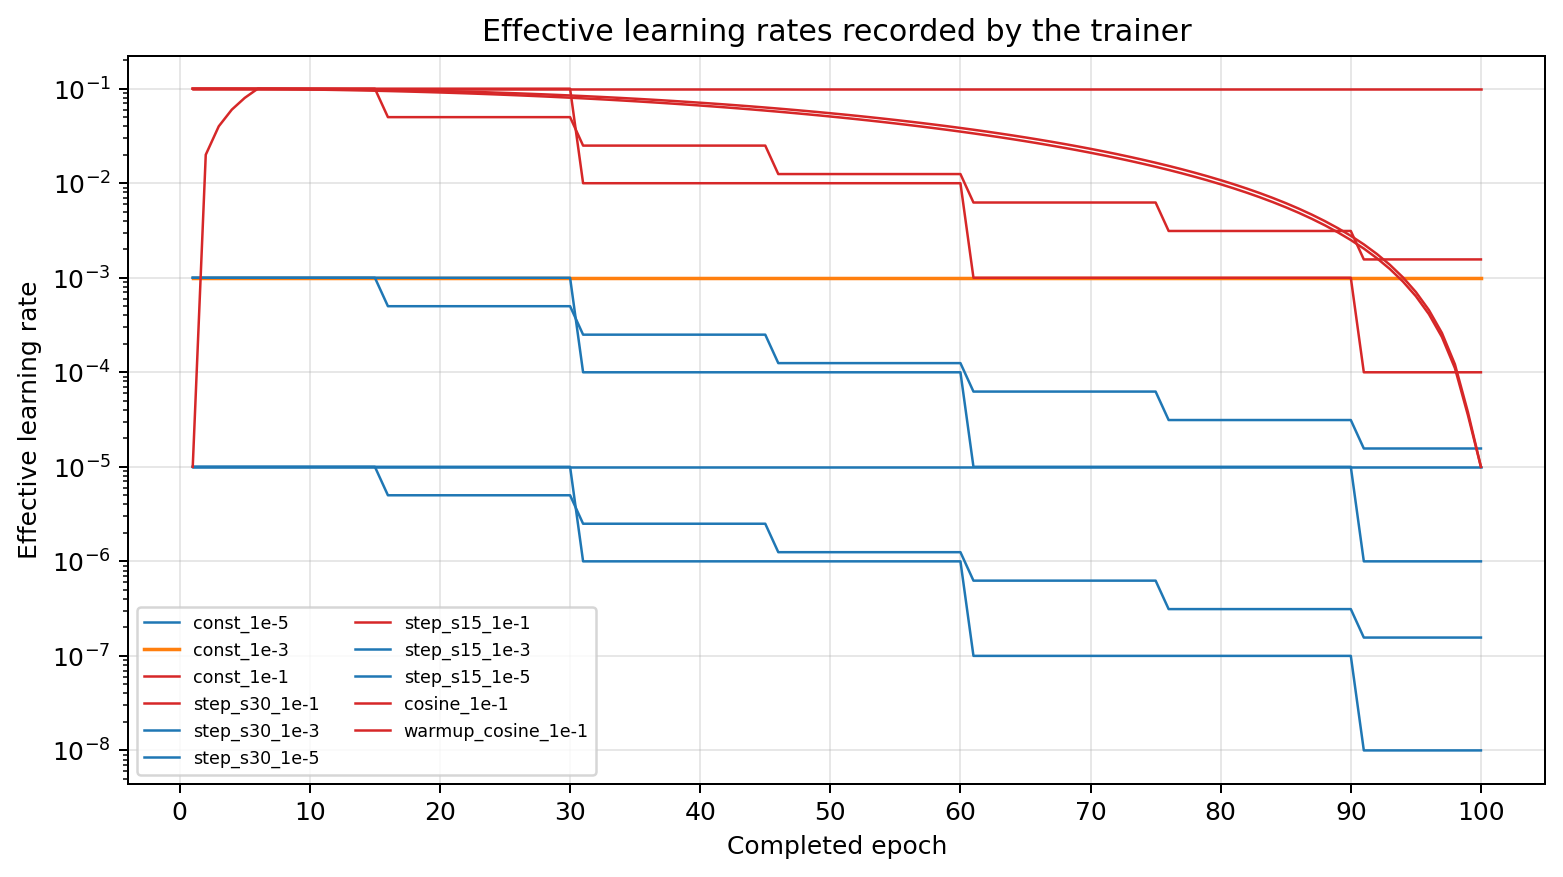
\includegraphics[width=0.90\linewidth]{Images/Chapter04/learning_rate/learning_rate_schedules.png}
    \caption{Effective learning rates from \texttt{epoch\_metrics.csv} for zero-based fold 0, plotted against completed epoch. The scheduler settings are deterministic and identical across folds. The logarithmic vertical axis makes the constant, step, cosine, and warm-up branches comparable.}
    \label{fig:04_learning_rate_schedules}
    \end{figure}

The high-rate candidates should be described as numerically unstable rather than as failed jobs. All 55 candidate-fold fits completed with finite diagnostic values and were included in the official ranking, but the five candidates that reach $10^{-1}$ have validation means from $5.577\times10^8$ to $2.131\times10^{17}$. The detailed diagnostics, presented in Figure \ref{fig:04_learning_rate_diagnostics}, provide an illustration of this.\\

In the top left panel, the bar chart represents the "worst-case scenario" for gradients in each run. For every candidate, it searches through all 100 epochs, all five folds and all layers of the network to find the single largest gradient value. We can see a clear separation between the stable and unstable candidates:
\begin{itemize}
    \item[-] for the stable rates ($10^{-5}$ and $10^{-3}$), the peak gradient norms are controlled, with the winning candidate maintaining a peak gradient of approximately $183$;
    \item[-] for the unstable rates ($10^{-1}$), the peak gradient norms grow uncontrollably, leading to a complete breakdown of the optimization trajectory.
\end{itemize}
Moving to the right panel, we observe the direct consequence on parameter movement: this plot measures the largest relative change made to the network's weights in a single optimization step. While the stable cases show well-behaved updates (around $0.017$ for the $10^{-3}$ candidate), the unstable $10^{-1}$ candidates exhibit update ratios approaching $100\%$. This means the optimizer attempts to displace weights by an amount equal to their entire existing magnitude in a single step, wiping out any learned representation.\\

The lower panels of Figure \ref{fig:04_learning_rate_diagnostics} provide a further check on the selected run.\\

The first plot shows the average gradient magnitude for each trainable layer at the very beginning of training (epoch 1) and at the end of training (epoch 100). The RMS gradient is a measure of how much the weights are being updated during training. A high RMS gradient indicates that the model is learning quickly, while a low RMS gradient suggests that learning has slowed down. The plot shows that the RMS gradient decreases over time, which is expected as the model converges to a solution. Indeed, we can see that the learning process starts strongly, with a peak norm of approximately $37$ at epoch 1; by epoch 100, the gradients have naturally decreased, settling in a stable range below $1.0$. This indicates that the model has learned a solid representation of the data and is performing refined parameter adjustments.\\

Regarding the post-activation variance, the lower-right panel shows the pooled population variance of the activations after the non-linear transformation at each layer. This is a measure of how much the activations vary across different inputs. In this case, we can see that at the beginning the signal variance grows as information passes deeper into the network, but at epoch 50 and epoch 100, the overall variance decreases and stabilizes. Crucially, the variance never collapses to zero and never explodes.\\
These two plots confirm that information is flowing effectively through all layers of the deep network for the entire duration of training and that the network does not suffer from vanishing or exploding activations.\\

\begin{figure}[H]
    \centering
    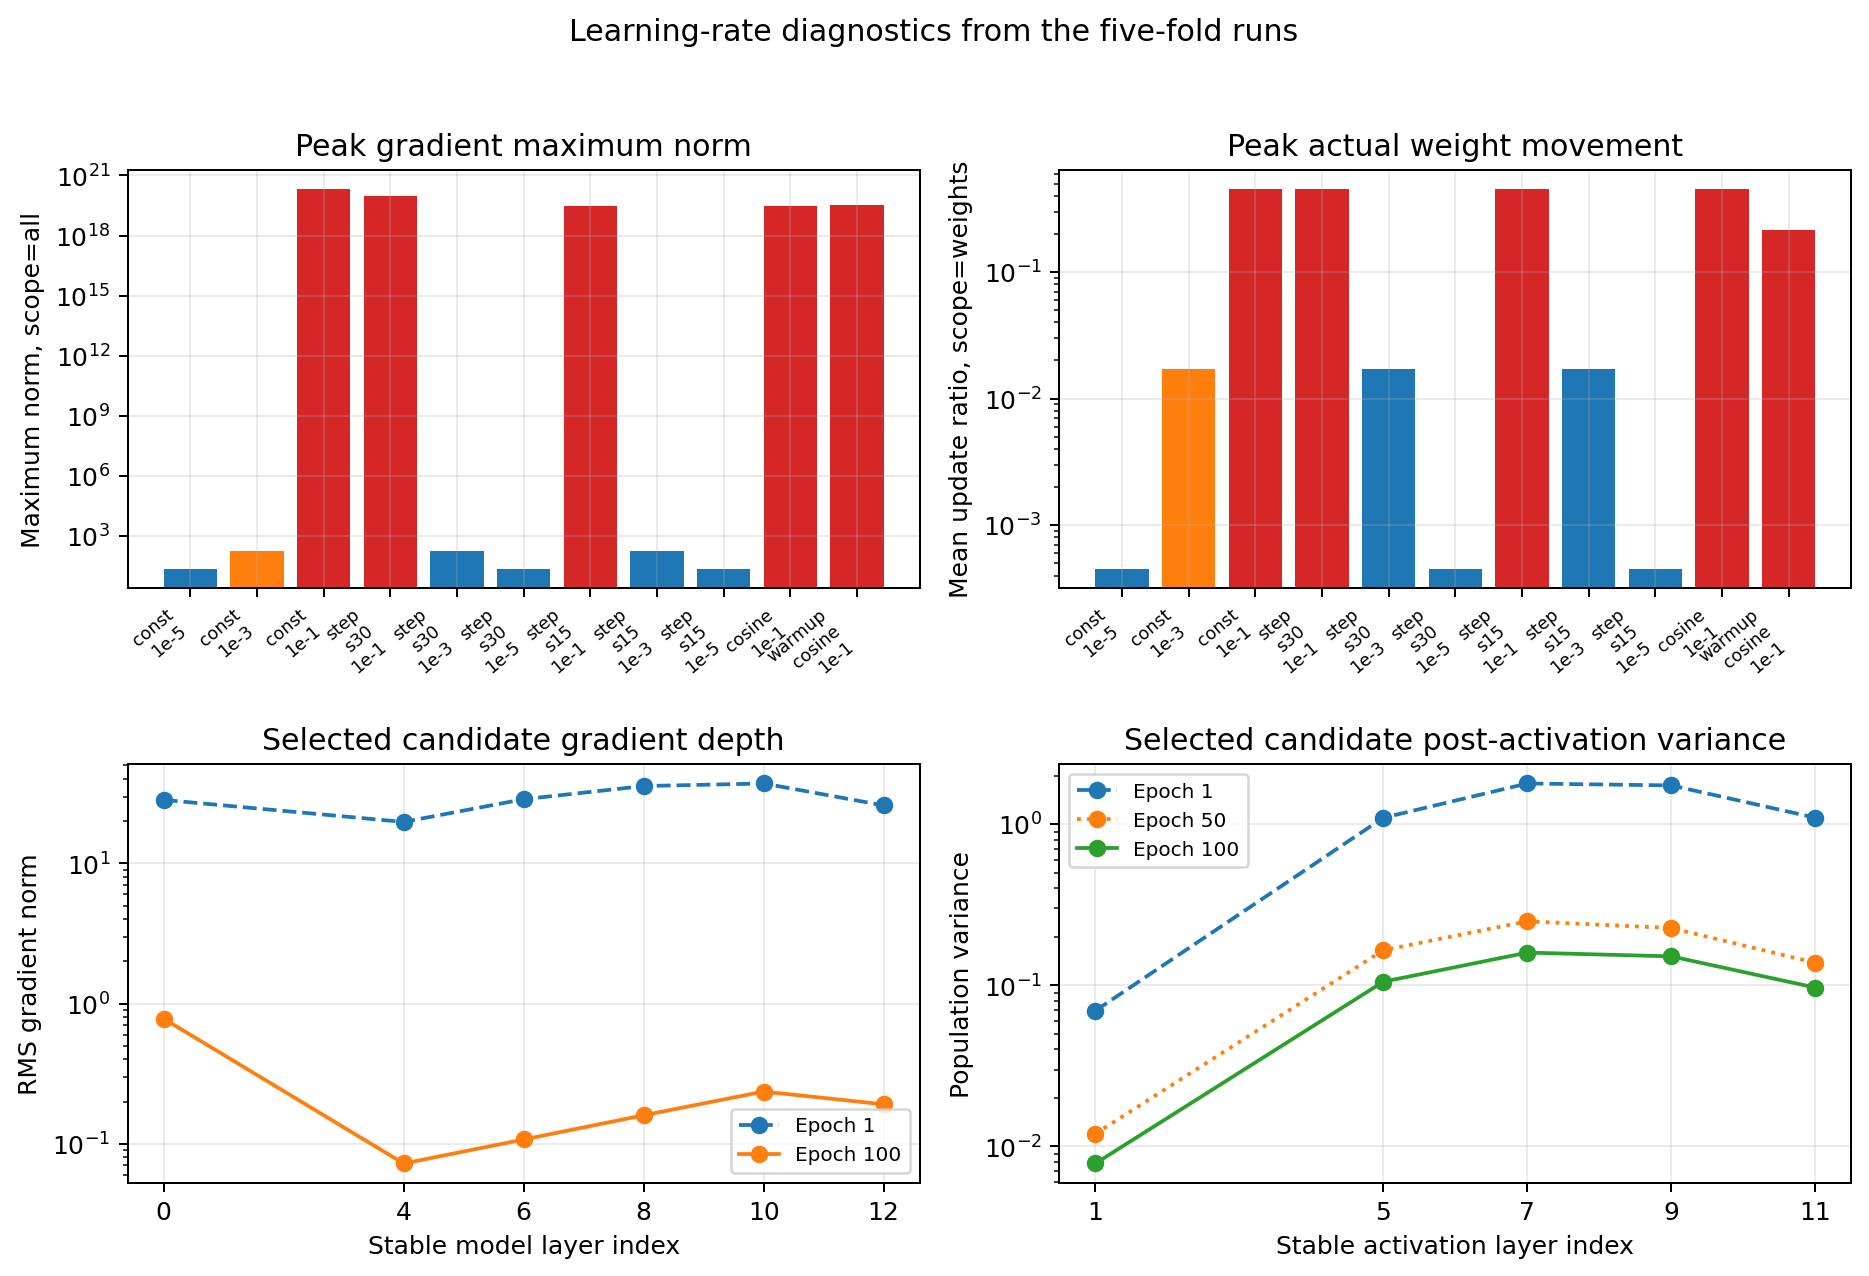
\includegraphics[width=0.95\linewidth]{Images/Chapter04/learning_rate/learning_rate_diagnostics.png}
    \caption{Learning-rate diagnostics from the complete five-fold run. The upper panels show the maximum over folds, layers, and epochs of \texttt{maximum\_norm} with \texttt{parameter\_scope=all} and of the actual \texttt{mean\_ratio} with \texttt{parameter\_scope=weights}. The lower-left panel shows the selected candidate's fold-averaged RMS gradient by stable model layer at epochs 1 and 100. The lower-right panel shows the selected candidate's pooled post-activation population variance at epochs 1, 50, and 100. All vertical axes are logarithmic.}
    \label{fig:04_learning_rate_diagnostics}
\end{figure}

The cross-validation experiment identifies the constant $10^{-3}$ learning rate as the clear winner, achieving a mean validation MSE of $0.003609\pm0.001335$. The analysis confirms that this learning rate represents a robust "sweet spot," offering rapid convergence without triggering the catastrophic numerical instability observed at higher rates like $10^{-1}$. After being refit on the full training set, this winning experimental candidate achieved a final test MSE of $0.003254$.\\

\subsection{Final production training}
\label{sec:04_final_training}

The preceding tuning experiments identified a set of optimal hyperparameters for the network architecture and optimizer. This final section details the development of the production training run, which combines these findings with a refined training protocol to achieve the best possible performance. Unlike the cross-validation used for tuning, this final training uses a single, fixed 90/10 split of the data for training and validation, with a normalization fitted only on the 1542 training samples and applied unchanged to the 171 validation samples and the subsequent test evaluation.\\

The final ordinary training was developed through a sequence of training trials rather than launched as a single fixed experiment. The first trial used a global batch size of 64 with the original range-based batching. Since the ordinary training split contains 1542 samples, this produced 24 batches of 64 samples and a final batch of only 6 samples, leading to wasted computational resources in our parallel MPI environment.\\

To solve this, we implemented a balanced batching strategy. Instead of creating as many full batches as possible, this strategy first determines the optimal number of batches, $K$, needed to keep the batch size as close to the target $B$ as possible. It then distributes the samples as evenly as possible among these $K$ batches. The exact size of each batch, $n_j$, is calculated as follows:
\begin{equation}
    K=\left\lceil\frac{n}{B}\right\rceil,
    \qquad q=\left\lfloor\frac{n}{K}\right\rfloor,
    \qquad r=n-Kq,
    \qquad
    n_j=\begin{cases}
        q+1, & j<r,\\
        q, & j\geq r,
    \end{cases}
    \quad j=0,\ldots,K-1,
    \label{eq:04_final_batch_partition}
\end{equation} 
where $n$ is the total number of training sample. Equation~\eqref{eq:04_final_batch_partition} gives 17 batches of 62 and 8 batches of 61 for the balanced 64-sample experiment, while $B=257$ produces six exact batches of 257. The former change removed the small tail without changing the 25 optimizer steps per epoch; the latter also reduced the number of updates per epoch to six. This distinction is important because the global batch size is not multiplied by the MPI rank count, and because the gradient synchronization in \texttt{CNN/src/model/CNNModel.cpp} weights each local gradient by its local sample count before dividing by the global count.\\

Early stopping is crucial for selecting the best model and preventing overfitting. However, our initial policy, which stopped training at the first sign of overfitting, proved to be too sensitive to normal training noise and often terminated runs prematurely. To address this, we implemented a more robust "20/20" policy. This new rule only stops training after the validation error has failed to improve for 20 consecutive epochs. This ensures that the model has truly converged and is not just experiencing a temporary fluctuation, leading to a much more reliable and stable model selection process.\\

The impact of these iterative improvements to the training protocol is documented Table \ref{tab:04_final_training_trials}. The table chronologically presents the results of several training trials, clearly showing how the refinement of the batching and early stopping policies led to progressively better and more stable outcomes. All errors in the Table are physical-unit MSE values, where "budget" is the maximum configured epoch count, "completed" is the length of the diagnostic history and "selected" identifies the restored validation-minimum checkpoint.\\

\begin{table}[h!]
    \centering
    \begin{tabularx}{\linewidth}{@{}Xrrrrrrr@{}}
        \hline
        Stage & $B$ & Budget & Completed & Selected & Train MSE & Val. MSE & Test MSE \\
        \hline
        Initial tail, \texttt{trial 1} & 64 & 200 & 200 & 162 & 0.001957 & 0.001714 & 0.001647 \\
        Balanced, \texttt{trial 2} & 64 & 200 & 191 & 139 & 0.002081 & 0.001719 & 0.001894 \\
        Exact batches, \texttt{trial 3} & 257 & 200 & 200 & 183 & 0.002614 & 0.002325 & 0.001998 \\
        First ratio, \texttt{trial 4} & 257 & 834 & 319 & 318 & 0.001518 & 0.001425 & 0.001512 \\
        First ratio, seed 0 & 257 & 834 & 5 & 5 & 0.011170 & 0.013795 & 0.009084 \\
        First ratio, seed 1 & 257 & 834 & 6 & 5 & 0.012426 & 0.013655 & 0.010525 \\
        20/20 policy, seed 0 & 257 & 834 & 834 & 820 & 0.000389 & 0.000552 & 0.000420 \\
        20/20 policy, seed 1 & 257 & 834 & 159 & 139 & 0.002924 & 0.004752 & 0.002381 \\
        20/20 policy, seed 42 & 257 & 834 & 834 & 797 & 0.000395 & 0.000435 & 0.000487 \\
        Final production (\texttt{trial 5}), seed 42 & 257 & 1200 & 860 & 797 & 0.000395 & 0.000435 & 0.000487 \\
        \hline
    \end{tabularx}
    \caption{Ordinary training results from the ten run directories under \texttt{results/ordinary-training}. Restored metrics come from \texttt{final\_metrics.csv}; budgets, batch construction and stopping policies come from metadata, and completed epochs from diagnostic histories. The final two seed-42 rows retain the same checkpoint; the increased budget is not an accuracy gain.}
    \label{tab:04_final_training_trials}
\end{table}

The first three trials demonstrate the effect of refining the batching strategy. While the initial move from a tailed to a balanced batch (\texttt{trial 2}) improved parallel efficiency, increasing the global batch size to a perfectly divisible 257 (\texttt{trial 3}) provided a more stable foundation for subsequent, longer training runs.\\

The most dramatic improvement came from refining the early stopping rule.  The trials labeled "First ratio" show that the original, sensitive policy often terminated training far too early (e.g., at epoch 5 or 6), resulting in very poor test performance (MSE > 0.009). In contrast, the robust "20/20" policy allowed the models to train for much longer, navigating through normal fluctuations in the validation loss to find a much better solution. This is best seen in the seed 0 and seed 42 runs, where the new policy allowed training to continue for over 800 epochs, leading to a more than 20-fold reduction in test MSE compared to the premature stops.\\

The final run (\texttt{trial 5}) combines all of these best practices: the optimal $B=257$ batch size, the robust "20/20" stopping policy, and an extended epoch budget of 1200. This culminated in the best performance of the sequence, identifying a model checkpoint with a test MSE of $0.000487$.\\

The physical-MSE histories show recurrent excursions in the unbalanced run that affect training and validation together. Figure~\ref{fig:04_final_trial_mse_comparison} uses the \texttt{training\_physical\_mse} and \texttt{validation\_physical\_mse} columns of \texttt{epoch\_metrics.csv}, evaluated after the updates at every epoch. In trial 1, the excursion at epoch 84 reaches training MSE $0.0210883$ and validation MSE $0.0218529$, rising from $0.0042626$ and $0.0039933$ at epoch 83 and returning to $0.0075658$ and $0.0069386$ at epoch 85. Balancing reduces these recurrent excursions but does not eliminate all fluctuations: trial 2 still reaches $0.0088347$ and $0.0090290$ at epoch 11, and $0.0086777$ and $0.0086519$ at epoch 12. Both curves remain below $0.008$ thereafter. All 200 and 191 recorded epochs are finite and use a constant effective learning rate of $10^{-3}$. The simultaneous movement of training and validation is consistent with a noisy update affecting the shared model rather than a validation-only increase in error.\\

\begin{figure}[h!]
    \centering
    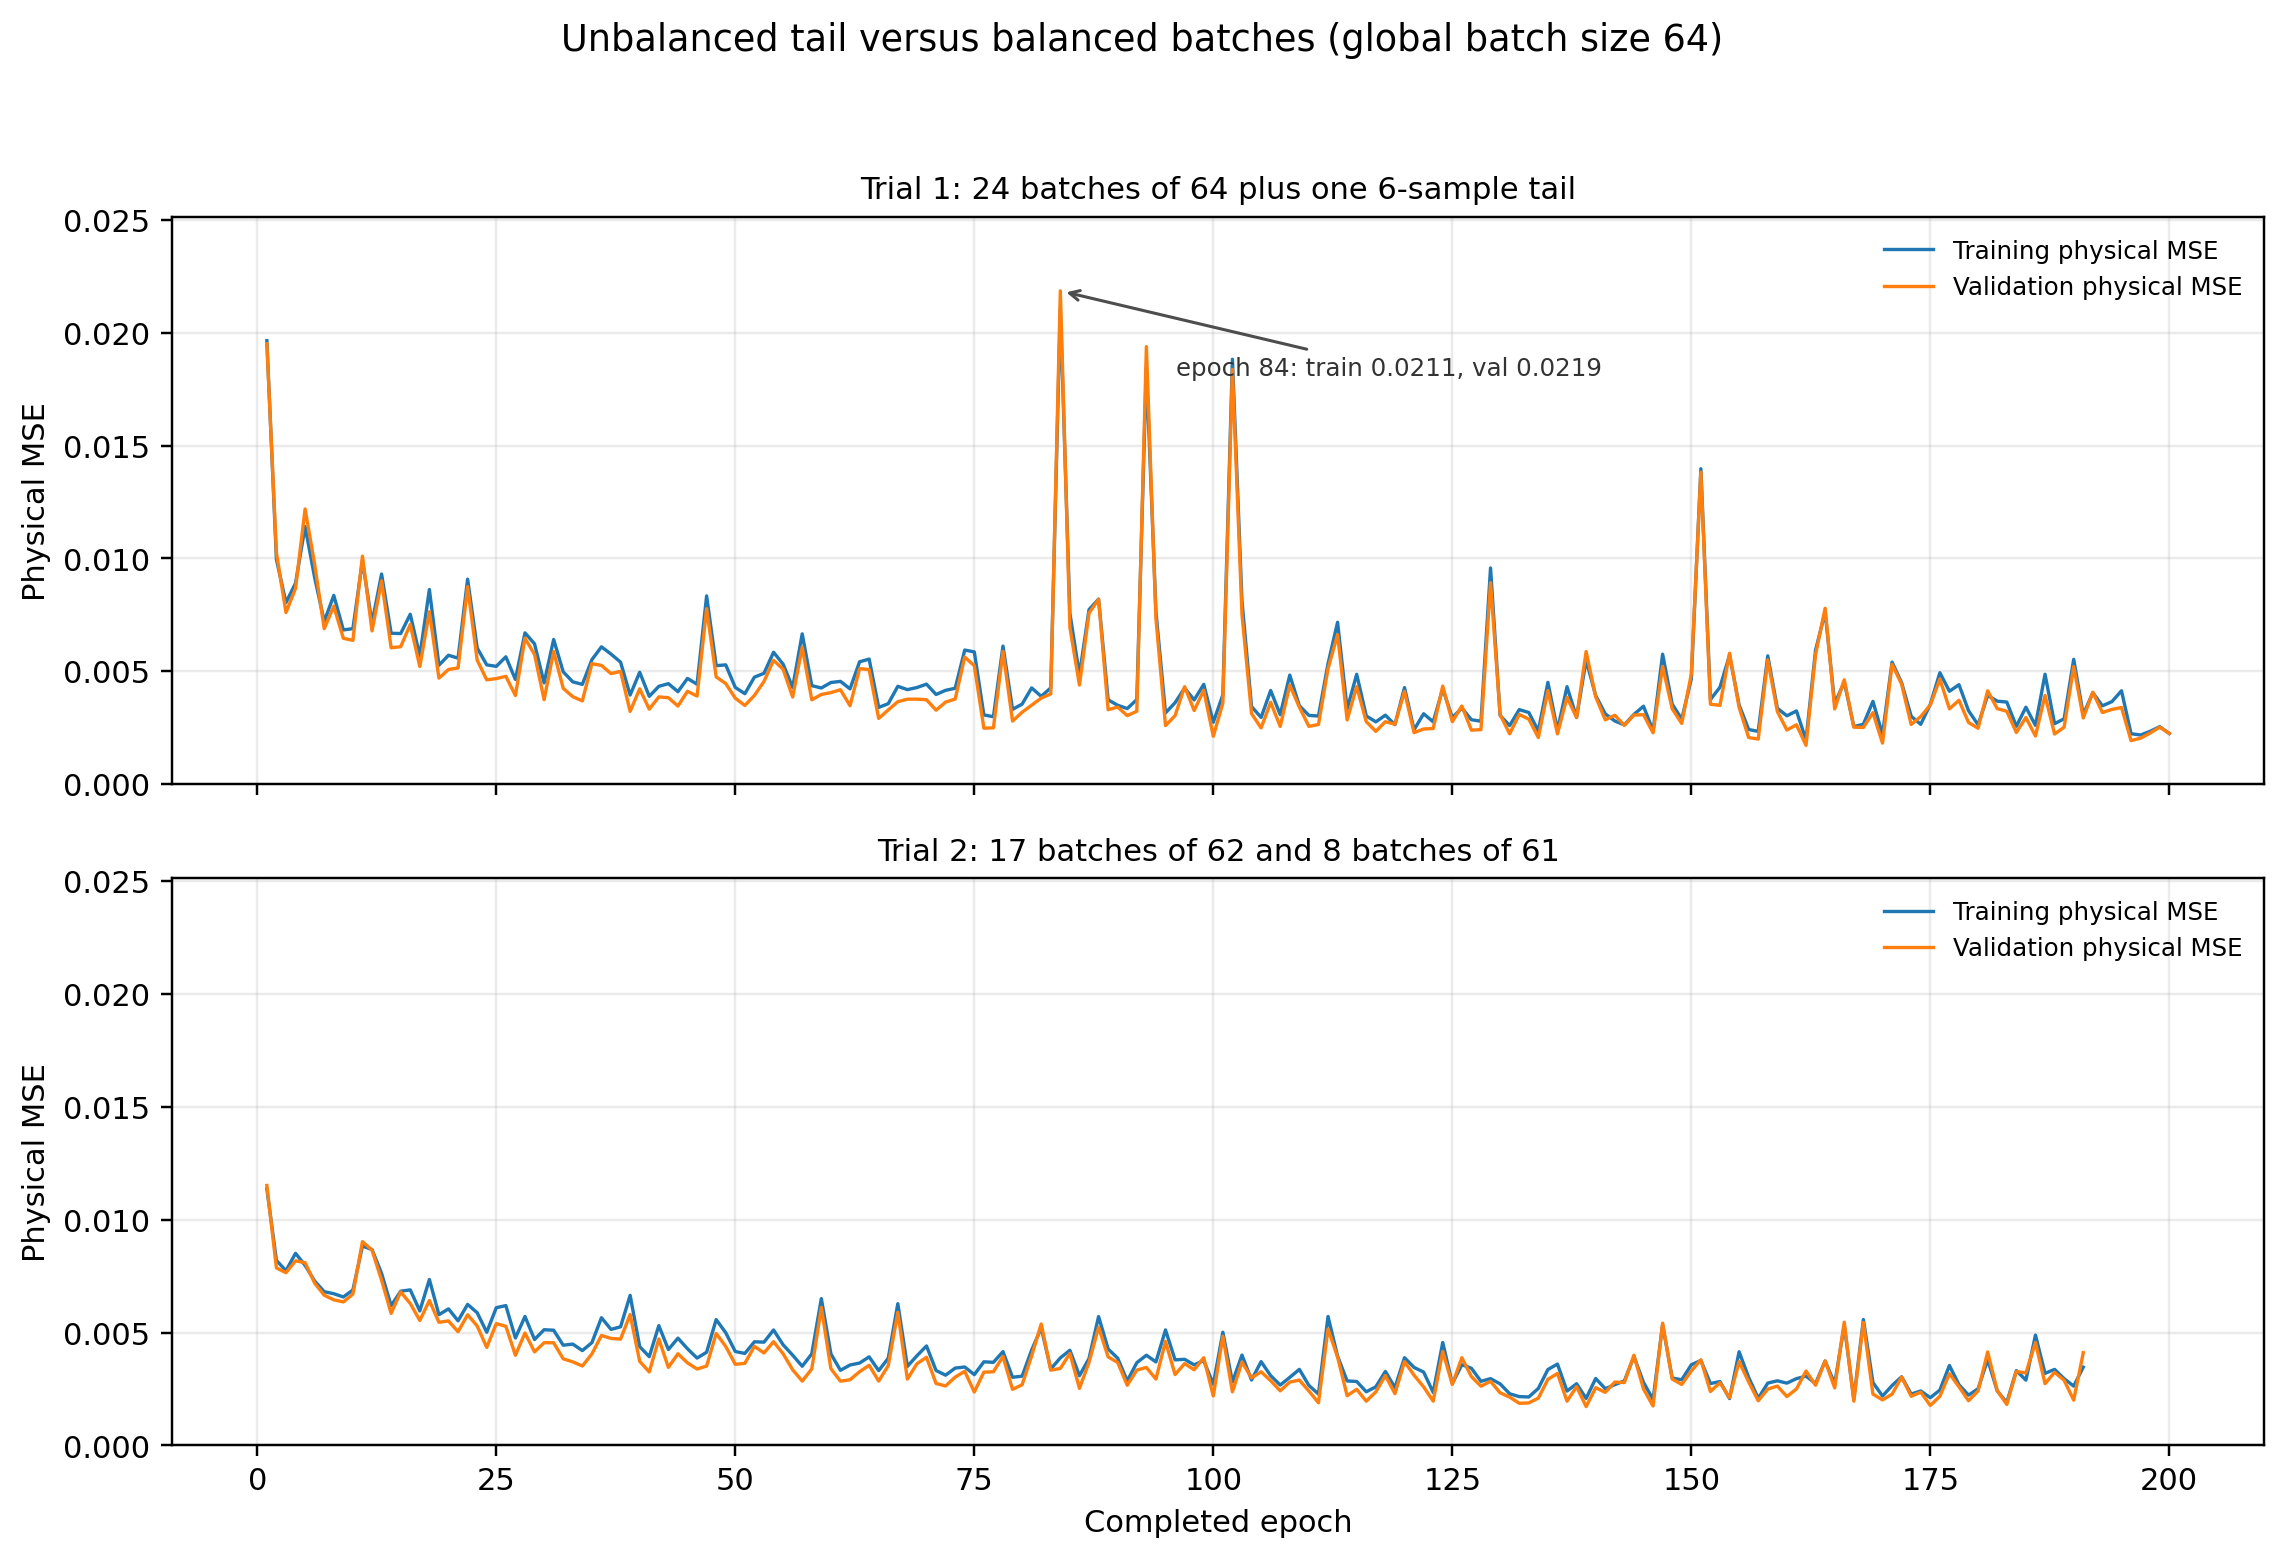
\includegraphics[width=0.69\linewidth]{Images/Chapter04/final_training/final_trial1_trial2_mse_comparison.png}
    \caption{Physical training and validation MSE for the two seed-42 runs at global batch size 64. The upper panel is trial 1 with 24 batches of 64 plus a 6-sample tail; the lower panel is trial 2 with 17 batches of 62 and 8 batches of 61. The common linear scale includes the full histories of 200 and 191 completed epochs. The annotation marks the epoch-84 excursion in trial 1. These are single-run histories, not fold averages; the standardized SIMM objective is not shown.}
    \label{fig:04_final_trial_mse_comparison}
\end{figure}

The gradient and parameter-update diagnostics give a more detailed view of the same excursion. Figure~\ref{fig:04_final_trial_gradient_update} uses \texttt{parameter\_scope=all} from \texttt{gradient\_norms.csv} and \texttt{parameter\_update\_ratios.csv}, combining weights and biases rather than isolating small bias denominators. Gradients are measured after weighted MPI synchronization and before clipping and the optimizer update; the actual update ratio in Equation~\eqref{eq:04_update_ratio} includes clipping, Adam moments and the current parameter scale. The left panel plots epoch-84 RMS gradient norms at stable indices 0, 4, 6, 8, 10 and 12, corresponding to the convolution and five dense layers. The convolution norm is $1.27083$ in trial 1 against $0.53502$ in trial 2, whereas the dense-layer profiles are much closer: the first dense values are $0.07483$ and $0.06975$. At epoch 85 the convolution norms rise to $2.96752$ and $1.09226$, respectively. The right panel follows the first dense layer's mean update ratio over each run's own completed history. At epoch 84 this ratio is actually lower in trial 1, $0.0012268$ against $0.0016265$, but at epoch 85 it reaches $0.0055988$ against $0.0026526$. The corresponding mean pre-update parameter norms lie between $46.60$ and $46.85$, with no near-zero denominator steps. Thus the diagnostics do not show a uniform increase in every layer at the MSE peak: the larger actual mean movement occurs in the following epoch. Moreover, the last convolution gradient norm at epoch 84 equals that epoch's maximum, $4.45210$, in the unbalanced run.\\

\begin{figure}[h!]
    \centering
    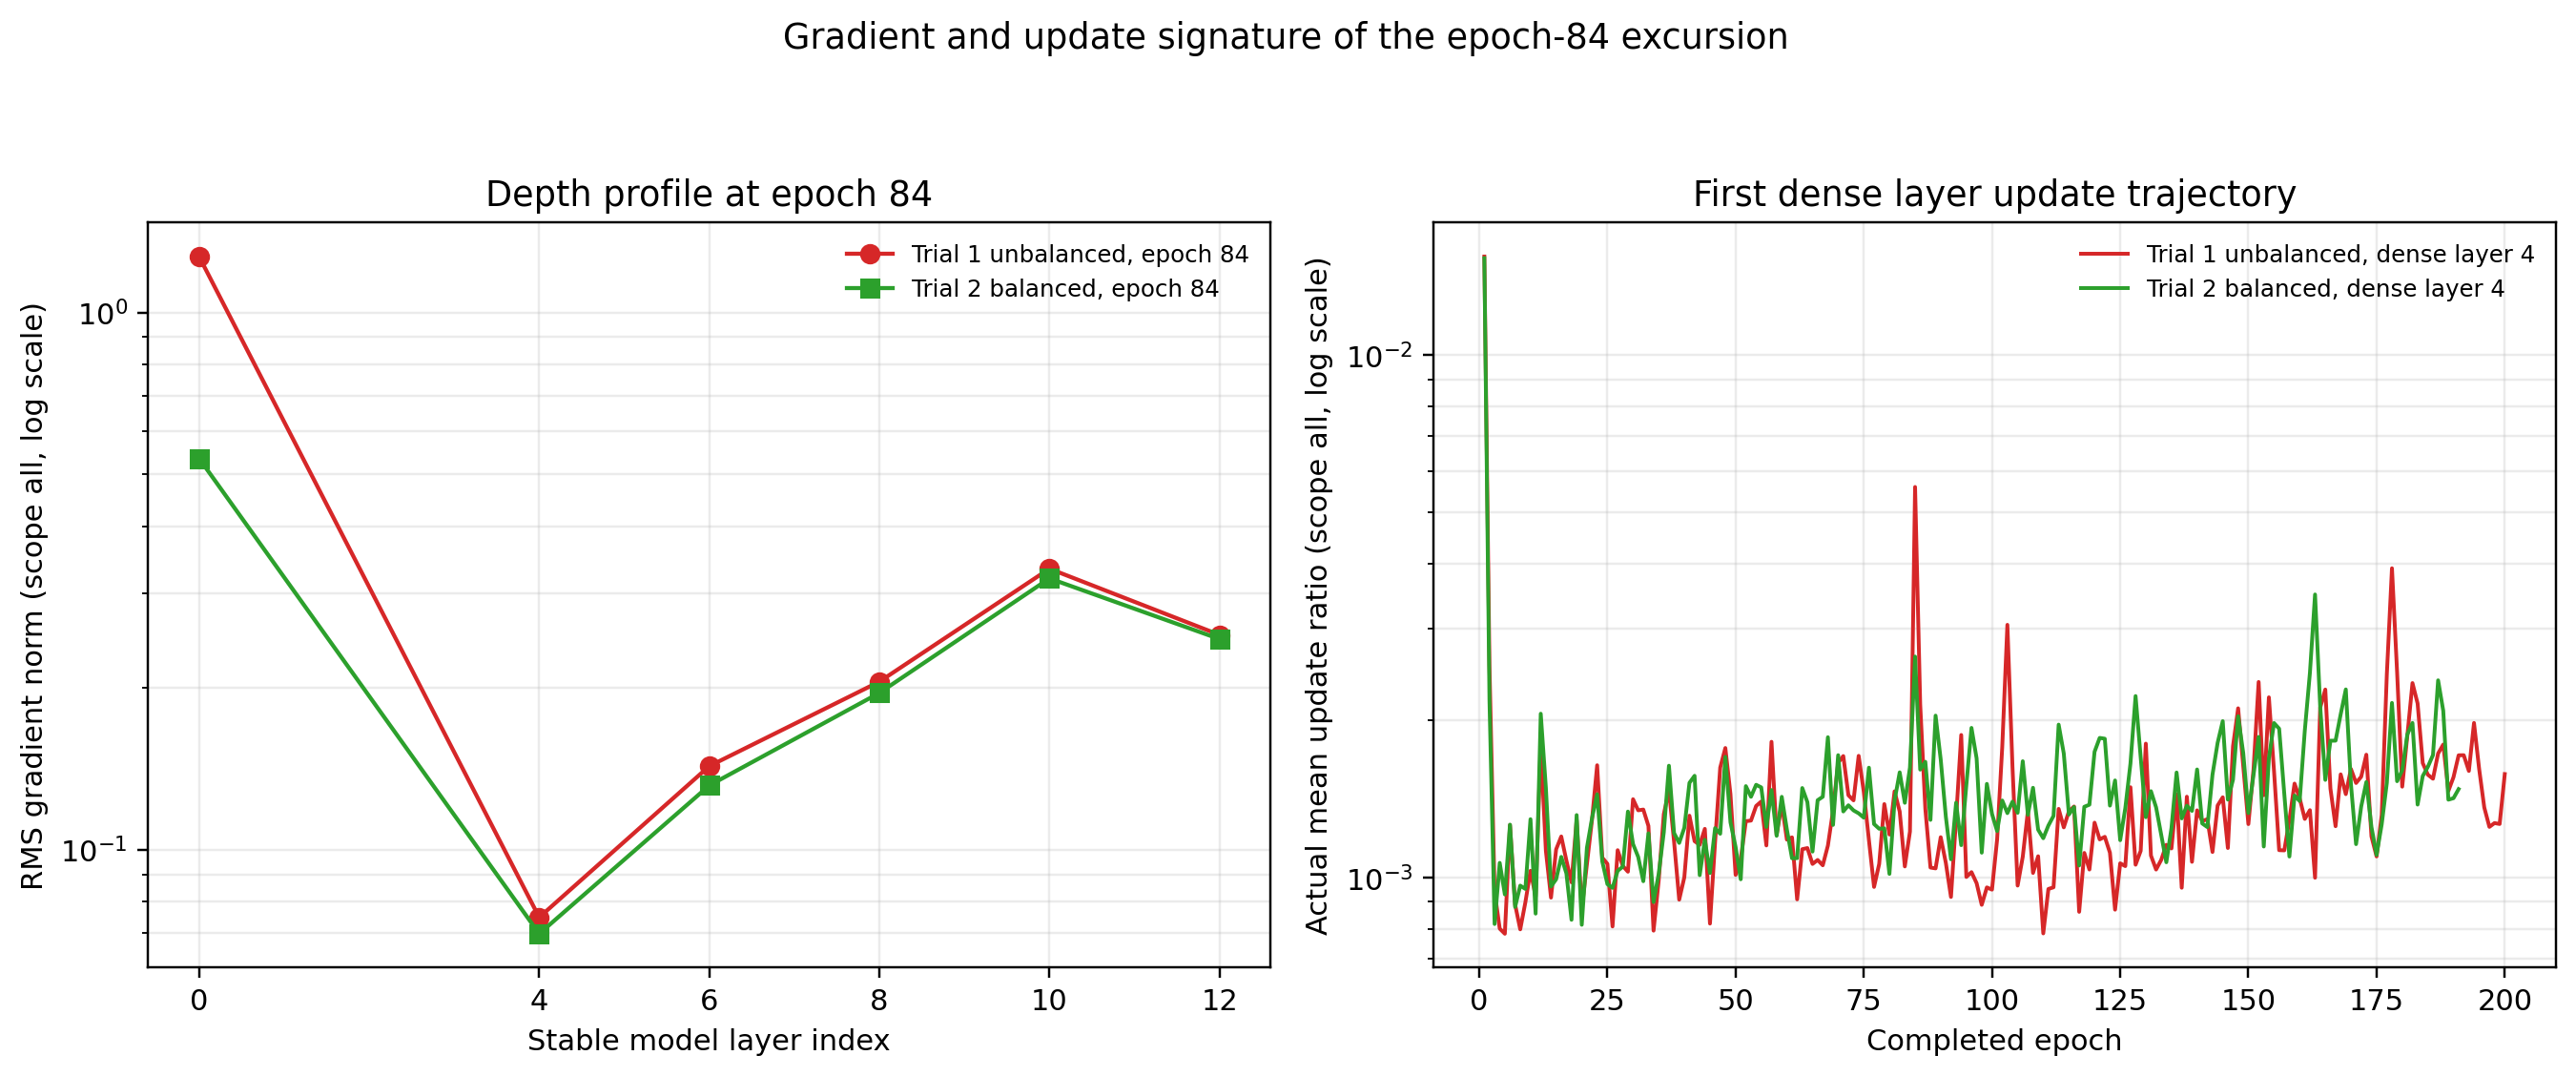
\includegraphics[width=0.98\linewidth]{Images/Chapter04/final_training/final_trial1_trial2_gradient_update.png}
    \caption{Diagnostics around the epoch-84 excursion. Left: synchronized, pre-clipping RMS gradient norms across all six trainable layers at epoch 84. Right: actual mean update ratio of the first dense layer, index 4, over 200 epochs for trial 1 and 191 for trial 2. Both vertical axes are logarithmic and use \texttt{parameter\_scope=all}. Red denotes the unbalanced run and green the balanced run.}
    \label{fig:04_final_trial_gradient_update}
\end{figure}

The reduction in recurrent excursions must be distinguished from an accuracy gain. Trial 1 restores epoch 162, with training MSE $0.0019568$, validation MSE $0.0017142$ and test MSE $0.0016466$; trial 2 restores epoch 139, with $0.0020810$, $0.0017195$ and $0.0018941$, respectively. Their validation minima are practically equal, and the balanced run does not improve the reported test error. We therefore retain balancing as a way of avoiding the very small final update, not as evidence of better predictive accuracy by itself. The comparison is limited to these two seed-42 trajectories and does not establish that all optimization noise has been removed.\\

The move to $B=257$ gives six exact batches because $1542=6\times257$. However, the 200-epoch trial then performs only 1200 Adam updates, compared with the 5000-update budget at $B=64$. Its selected validation MSE is $0.0023254$ and its test MSE is $0.0019978$, so increasing the batch size alone does not improve the matched-epoch result. To allow a comparable number of updates, we increase the budget to 834 epochs, corresponding to $834\times6=5004$ planned updates. This is a budget comparison, not a claim that every run completes those updates. With the earlier stopping rule, the seed-42 trial stops at epoch 319 and retains epoch 318, with validation MSE $0.0014248$ and test MSE $0.0015124$. The early termination of this longer configuration motivates examining the stopping policy.\\

The overfitting check is based on the physical training and validation MSE evaluated after the optimizer updates at every epoch. An epoch satisfies the gap condition in Equation~\eqref{eq:04_final_overfit_rule} when
\begin{equation}
    \mathrm{MSE}_{\mathrm{val},e}
    > (1+\rho)\,\mathrm{MSE}_{\mathrm{train},e},
    \qquad \rho=0.15,
    \label{eq:04_final_overfit_rule}
\end{equation}
but this condition is not sufficient by itself in the current implementation. The earlier \texttt{first\_ratio} rule stopped at the first qualifying epoch. With the 834-epoch budget, it terminates the seed-0 and seed-1 runs at epochs 5 and 6, respectively, and both retain epoch 5. Their selected validation MSE values are still $0.0137949$ and $0.0136545$, with test MSE $0.0090836$ and $0.0105255$. These short histories show why a gap during the initial optimizer transient should not automatically be interpreted as sustained overfitting.\\

The revised policy retains the $15\%$ ratio but uses a minimum of 20 epochs and a patience of 20 consecutive qualifying epochs. In \texttt{Trainer}, the streak resets before epoch 20, whenever validation reaches a new minimum, or whenever validation MSE is at most $1.15$ times training MSE. Otherwise it increases by one. A parameter snapshot is stored at every new validation minimum, and the best parameters are restored before the final metrics are recomputed. With this policy and the 834-epoch budget, seed 0 completes the budget and selects epoch 820, seed 1 stops at epoch 159 and selects epoch 139, and seed 42 completes the budget and selects epoch 797. Their validation MSE values are $0.0005521$, $0.0047519$ and $0.0004354$, respectively. The policy permits substantially longer optimization than the first-ratio rule, particularly for seeds 0 and 1, but the remaining variation shows that it does not remove sensitivity to initialization and the holdout split.\\

The final production configuration uses a $5\times5$ convolution from one input channel to eight output channels, with stride five and no padding. Flattening produces 7200 features; concatenating Reynolds number and angle of attack gives the 7202 inputs to the dense head $(1024,512,256,128,1)$. LeakyReLU with negative slope $0.05$ follows the convolution and each hidden dense layer, while the output is linear. This is the architecture constructed by the current \texttt{make\_single\_trial} in \texttt{CNN/main.cpp}. The recorded final production run, \texttt{trial-5\_slurm-56688207}, belongs to the \texttt{re-tuning} experiment at source revision \texttt{d9c1b4994e3c}, where a separate driver generated these trials; its metadata matches the current production recipe, rather than establishing that the current executable produced the archived run. It uses Adam with learning rate $10^{-3}$, moment coefficients $0.9$ and $0.999$, $\epsilon=10^{-8}$, zero weight decay, physics weight $0.10$, no dropout or L1 or L2 penalty, componentwise gradient clipping at 1, global batch size 257, seed 42 and 64 MPI ranks. Its recorded maximum is 1200 epochs, whereas the default in \texttt{CNN/main.cpp} is 200 epochs.\\

Increasing the seed-42 budget from 834 to 1200 epochs allows the stopping rule to finish at epoch 860 in trial 5, the final production run. The 834-epoch run already selects epoch 797, and trial 5 restores that same checkpoint. Its history through epoch 834 matches the seed-42 834-epoch run, and both restore identical parameters. The extra budget therefore allows termination under the stopping policy, but does not lower the retained validation minimum or constitute an accuracy improvement.\\

The final history begins with a finite initial transient: training and validation MSE are $0.2116009$ and $0.2113380$ at epoch 1, fall to $0.0390008$ and $0.0383861$ at epoch 2, and reach $0.0089447$ and $0.0087936$ at epoch 3. At the retained epoch 797 they are $0.000394531$ and $0.000435441$. Training continues until epoch 860, whose un-restored training and validation MSE are $0.000648353$ and $0.000960955$. The final qualifying streak is epochs 841--860, not the 20 epochs immediately following the selected checkpoint, because intervening returns below the ratio reset the counter. Production therefore performs 5160 optimizer updates, while the selected parameters come from update 4782. Figure~\ref{fig:04_final_training_history} shows the complete physical-MSE history in linear and logarithmic views and distinguishes selection from termination. The standardized SIMM objective, which is $2.42682$ at epoch 1, is a different quantity and is not plotted on the physical-MSE axes.\\

\begin{figure}[h!]
    \centering
    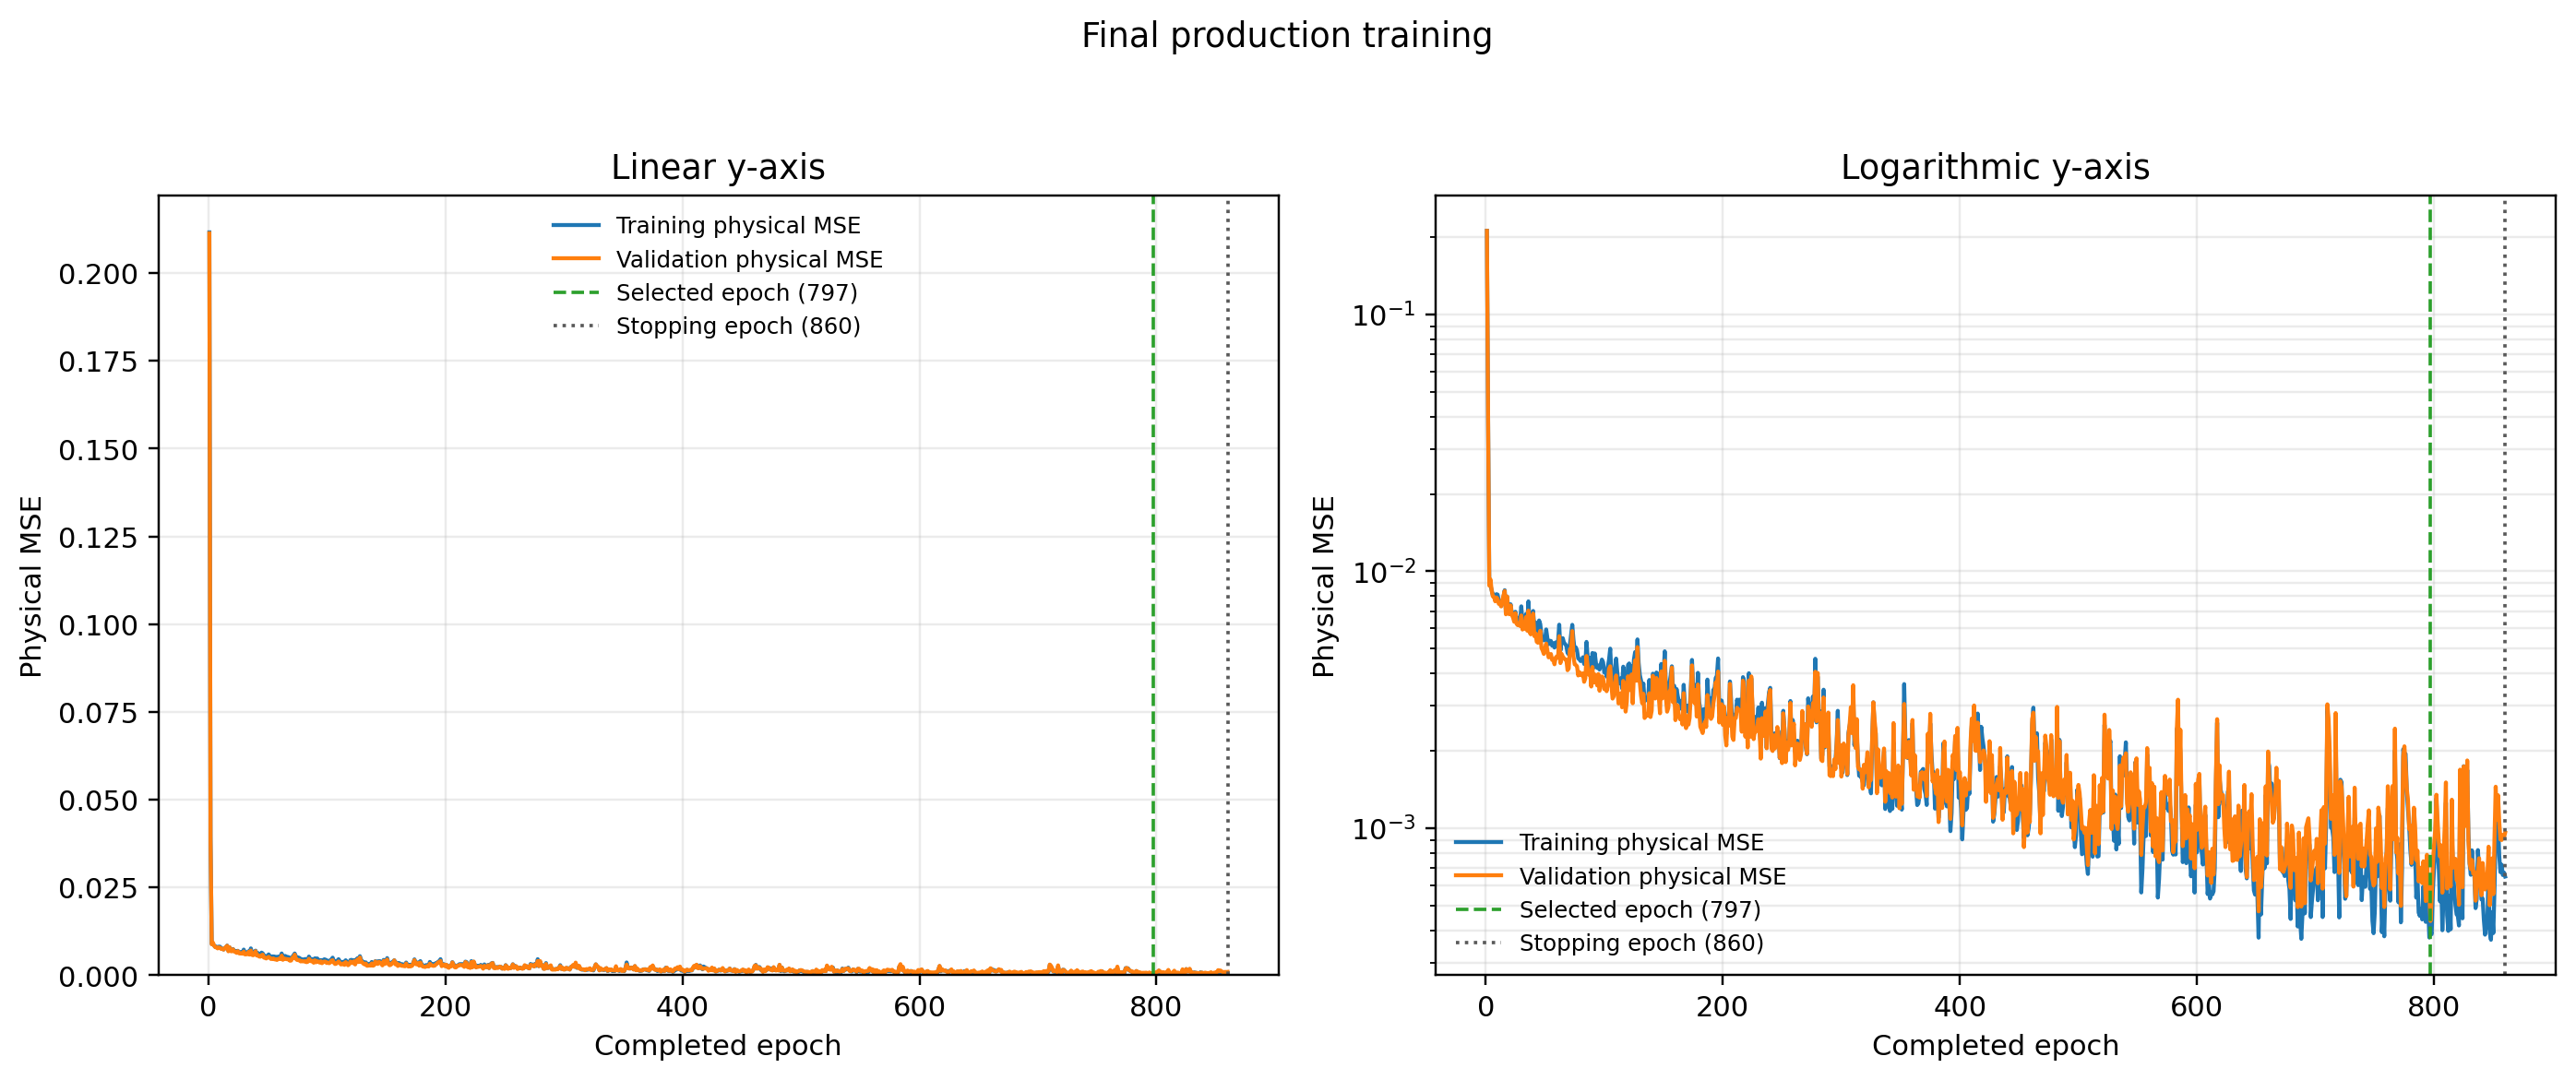
\includegraphics[width=0.95\linewidth]{Images/Chapter04/final_training/final_training_history.png}
    \caption{Physical training and validation MSE for the final production run, \texttt{trial-5\_slurm-56688207}. The left panel uses a linear y-axis and the right panel a logarithmic y-axis; both contain all 860 completed epochs. The dashed line marks selected epoch 797 and the dotted line stopping epoch 860. The standardized SIMM objective is not shown.}
    \label{fig:04_final_training_history}
\end{figure}

The production diagnostics provide a complementary check on this convergence. At epoch 1, the all-parameter RMS gradient norms range from $20.0543$ to $41.1596$ across the six trainable layers. At epoch 797, the convolution norm is $0.59468$, while the five dense-layer norms are $0.02963$, $0.03558$, $0.05370$, $0.09576$ and $0.08463$ in model order. The actual mean update ratios at the selected epoch range from $0.000210$ to $0.000940$; the largest over the production history is $0.03581$ at the first dense layer in epoch 1, with no near-zero denominator events in the all-parameter rows. At activation indices 1, 5, 7, 9 and 11, the globally aggregated post-activation population variances change from $(0.10460,0.97827,1.69423,1.50668,0.96488)$ to $(0.00346,0.06938,0.14887,0.15338,0.10306)$. The smaller gradients, parameter movements and activation variances accompany lower physical error, rather than a late numerical runaway. Across the ten runs, the recorded diagnostics are finite and the activation histogram populations are consistent with the recorded tensor sizes.\\

The restored production model is then evaluated on the 429-sample test set, separated according to the same $10^\circ$ angle threshold used by the SIMM mask. A sample belongs to the high-angle group only when $|\alpha|>10^\circ$, so samples exactly at $\pm10^\circ$ remain in the low-angle group. Table~\ref{tab:04_final_angle_results} reports the complete split. The high-angle MSE is $0.000552233$ larger than the low-angle MSE and $2.374$ times as large. Taking square roots gives RMSE values $0.02005$ and $0.03089$ for the low- and high-angle groups. The high-angle samples represent $66/429=15.38\%$ of the test set but account for approximately $30.15\%$ of the total squared error. This larger error occurs in the regime where the SIMM relation is inactive, although the split alone cannot identify the mask as its cause; the two groups also differ in sample count and input regime.\\

\begin{table}[h!]
    \centering
    \scriptsize
    \setlength{\tabcolsep}{4pt}
    \begin{tabular}{lrrrr}
        \hline
        Test subset & Samples & Physical MSE & Difference vs. low & High / low MSE \\
        \hline
        Overall & 429 & 0.000486795 & -- & -- \\
        $|\alpha|\leq10^\circ$ & 363 & 0.000401836 & -- & -- \\
        $|\alpha|>10^\circ$ & 66 & 0.000954069 & +0.000552233 & 2.374 \\
        \hline
    \end{tabular}
    \caption{Angle-of-attack split of the final production test metrics read from \texttt{test\_metrics.csv}. The high-angle difference and ratio are computed from the two stored subset MSE values; no per-sample residual spread was recorded.}
    \label{tab:04_final_angle_results}
\end{table}

Figure~\ref{fig:04_final_test_mse_by_angle} gives the same comparison graphically and includes the overall test MSE as a reference. It is a comparison of two physically defined test subsets, not a comparison of two separately trained models. The test set was not used to select the stopping epoch, and the figure therefore describes the aggregate subset error of the one restored production model rather than a new tuning criterion.\\

\begin{figure}[h!]
    \centering
    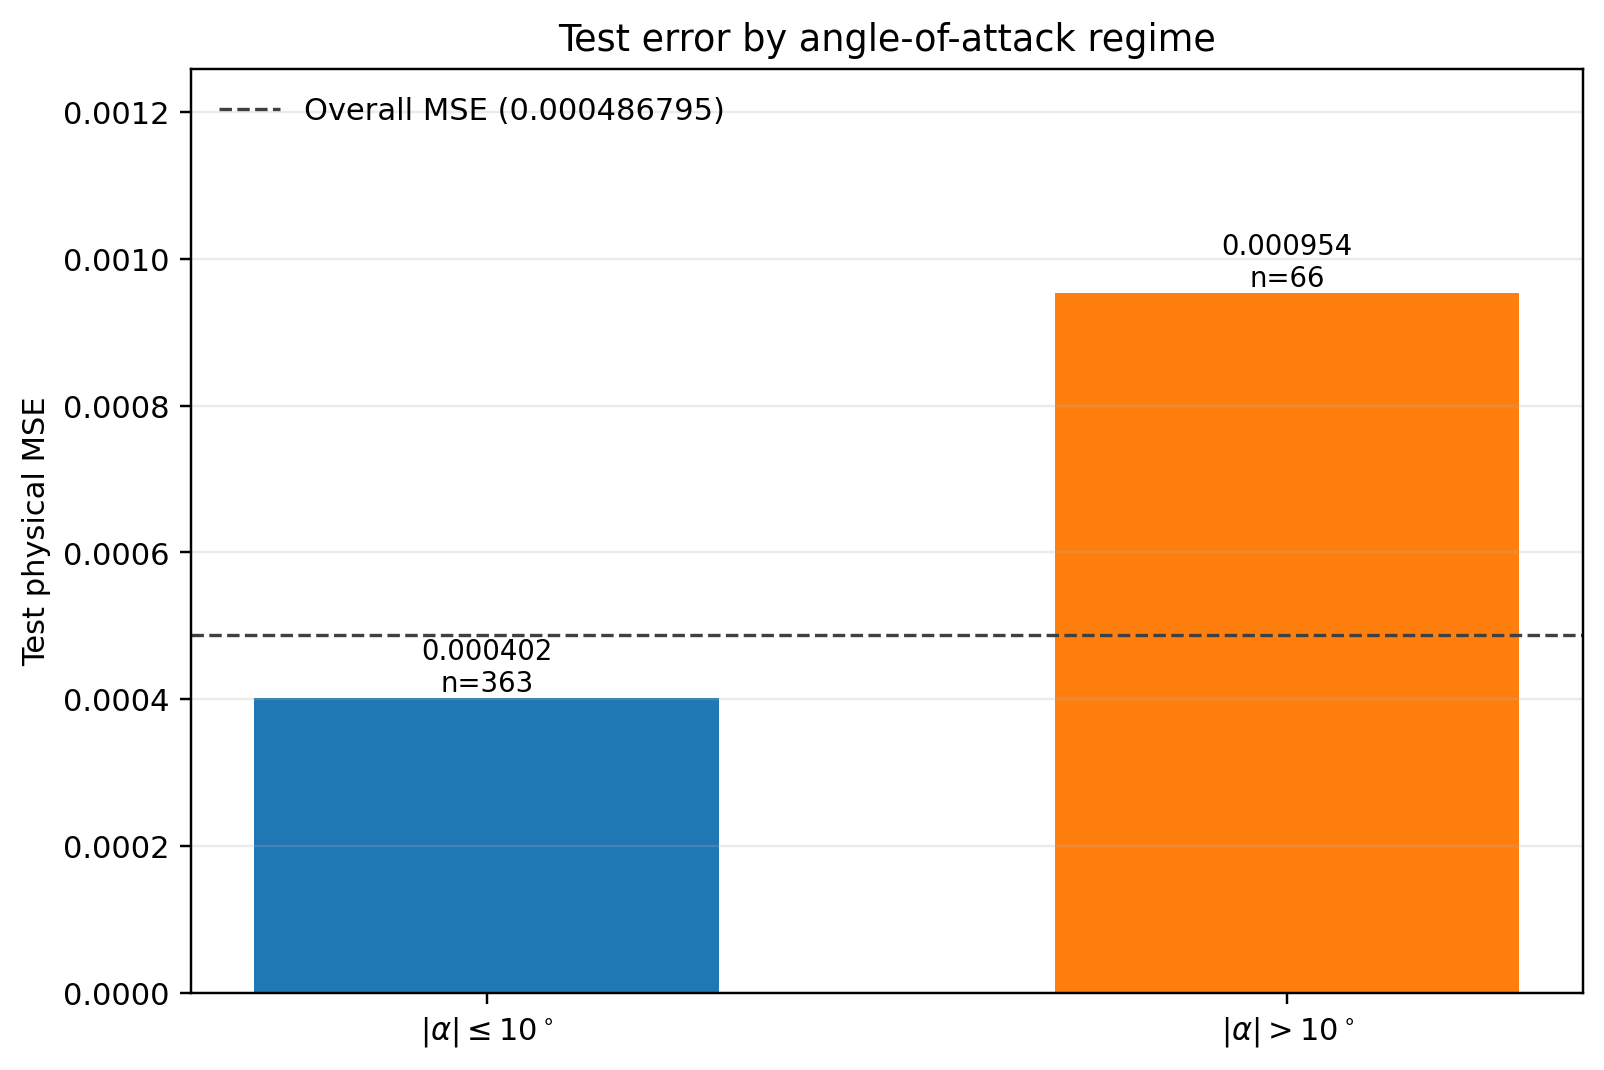
\includegraphics[width=0.78\linewidth]{Images/Chapter04/final_training/test_mse_by_angle.png}
    \caption{Post-training test physical MSE for the restored seed-42 production model, split into the low-angle ($|\alpha|\leq10^\circ$) and high-angle ($|\alpha|>10^\circ$) regimes. The bars are based on 363 and 66 samples, respectively, and the dashed line marks the overall MSE over all 429 test samples.}
    \label{fig:04_final_test_mse_by_angle}
\end{figure}

The final values should not be compared with every cross-validation value without qualification. The tuning experiments use fold-specific normalization and approximately 80 percent of the 1713 training samples in each fold, whereas ordinary training uses a 90/10 split and a different update budget. The final numbers describe the recorded large-topology production configuration with validation-based checkpoint restoration. Although each run evaluates the test set only after training, test metrics were recorded for all development trials; these artifacts do not establish that the test set was never inspected during development. We therefore report the production result as a post-training test evaluation, not as an independently untouched estimate for the entire tuning campaign.\\

\subsection{Tuning summary and conclusions}
\label{sec:04_tuning_conclusions}

The tuning campaign detailed in this chapter systematically refined the surrogate model, providing several key insights into the architecture and training protocols required for high-fidelity aerodynamic prediction.\\

The largest improvement among the structural choices came from replacing the initial $(128,64)$ dense head with the selected topology \texttt{conv5x5-dense-1024-512-256-128}. Its cross-validated physical MSE was $0.004560$, compared with $0.006010$ for the topology baseline, and the improvement was observed in all five folds. In addition to this, the tuning experiments identified Adam as the best optimizer at the tested rate $10^{-5}$, with a mean validation MSE of $0.004427$. The activation comparison selected LeakyReLU with $\alpha=0.05$ and the learning-rate search selected a constant Adam rate of $10^{-3}$, which reduced the cross-validated error to $0.003609$ for that experiment. These choices are supported not only by the mean scores, but also by finite diagnostics, small actual update ratios, and the absence of late-epoch divergence in the selected candidates.\\

The regularization results were different from what might be expected for a large network. Both dropout and weight penalties increased the recorded validation error, and the physics-weight sweep also selected the zero-weight reference. Nevertheless, to embed domain-specific physical grounding into the network, the moderate physics weight $\lambda=0.10$ was chosen for the final production model: its validation error increase over the unconstrained baseline was negligible ($+0.000028$) relative to fold variability, while preserving structural consistency with Thin-Airfoil Theory in the linear regime.\\

Ultimately, the final production model, combining the large topology with the refined training protocol, Adam at $10^{-3}$, and the $\lambda=0.10$ SIMM prior, produced an excellent final test MSE of $0.000487$. The 1200-epoch maximum was not exhausted: the run stopped at epoch 860, and the longer budget did not improve on the checkpoint already obtained with the 834-epoch budget. Crucially, when evaluating the final test predictions across aerodynamic regimes, the price of the physical constraint is clearly quantified: test samples with an angle of attack greater than $10^\circ$ ($|\alpha|>10^\circ$, $n=66$) produced a physical MSE of $0.000954$, which is nearly $2.4\times$ higher (almost double) than the physical MSE of $0.000402$ achieved on samples in the linear regime ($|\alpha|\leq 10^\circ$, $n=363$). This disparity occurs because the analytical thin-airfoil relation ($C_L\approx 2\pi\alpha$) is strictly valid and active only for $|\alpha|\leq 10^\circ$; beyond this threshold, flow separation and stall introduce strong aerodynamic non-linearities where the surrogate model must rely entirely on data-driven learning without an analytical prior.\\

Overall, the experiments show that surrogate accuracy depends on the joint choice of topology, optimizer, activation, learning rate, batch construction and stopping policy rather than on adding regularization indiscriminately. They also show why numerical diagnostics and explicit provenance are necessary: a low validation value is meaningful only when the topology, split, metric and training configuration that produced it are stated alongside the result.